\documentclass[a4paper]{article}

\usepackage{amsmath}
\usepackage{amssymb}
\usepackage{stellar}
\usepackage{parskip}
\usepackage{fullpage}
\usepackage{wrapfig}
\usepackage{witharrows}
\usepackage{cancel}
\usepackage{xfrac}
\usepackage{multirow}

\WithArrowsOptions{displaystyle}
\usetikzlibrary{decorations.pathmorphing, arrows.meta}

% Cancel color
\renewcommand{\CancelColor}{\color{red}}

\newcommand{\norm}[1]{\left\lVert#1\right\rVert}

\title{Appunti di Analisi Numerica}
\author{Paolo Bettelini}
\date{}

\begin{document}

\maketitle
\tableofcontents

\section{Fondamenti di algebra lineare numerica}

\subsection{Matrici speciali e forme normali}

\begin{snippettheorem}{Determinante matrice di Vandermonde}
    Sia \(V\) una matrice di Vandermonde. Allora
    \[
        \det V = \prod_{1 \leq i < j \leq n}(z_j - z_i)
    \]
\end{snippettheorem}

Quindi è invertibile se e solo se \(i \neq j \implies z_i \neq z_j\).

\begin{snippetproof}{Determinante matrice di Vandermonde}
    Procediamo per induzione.
    \begin{enumerate}
        \item \emph{Caso base:} se \(n=1\), allora \(\det V = \det [1] = 1\).
        \item \emph{Passo induttivo:} supponiamo che la tesi valga per \(n-1\).
            Allora possiamo calcolare il determinante usando l'espansione di Laplace
            \[
                \renewcommand{\arraystretch}{1.4}
                V = \left(
                    \begin{array}{cccc @{\hspace{1em}} | @{\hspace{1em}} c}
                        1 & z_1 & \dots & z_1^{n-2} & z_1^{n-1} \\
                        1 & z_2 & \dots & z_2^{n-2} & z_2^{n-1} \\
                        \vdots & \vdots & \ddots & \vdots & \vdots \\
                        1 & z_{n-1} & \dots & z_{n-1}^{n-2} & z_{n-1}^{n-1} \\
                        \hline
                        1 & z_n & \dots & z_n^{n-2} & z_n^{n-1}
                    \end{array}
                \right)
            \]
            Abbiamo \[
                \det V_n = \sum_{k=0}^{n-1} {(-1)}^{n+(k+1)}z^k_n M_k =
                \sum_{k=0}^{n-1} A_k z_n^k
            \]
            dove \(M_k\) è il minor ottenuto togliendo l'ultima riga e la colonna \(k+1\) e quindi
            \(A_k = {(-1)}^{n+(k+1)}M_k\).
            Quindi il determinante è un polinomio \(P(z)\) di grado \(n-1\) la cui potenza massima
            \(z^{n-1}_n\) corrisponde alla colonna \(n\), cioè \(M_{n-1} = \det V_{n-1}\). Otteniamo quindi l'espansione
            \[
                \det V_n = z_n^{n-1} \det V_{n-1} + \sum_{k=0}^{n-2} V_k z_n^k
            \]
            Per ipotesi induttiva, \[
                \det V_{n-1} = \prod_{1 \leq i < j \leq n-1} (z_j - z_i)
            \]
            che è il coefficiente del grado massimo \(z_n^{n-1}\).
            Notiamo ora che se avessimo \(z_n = z_k\) per qualche \(k<n\), allora due righe della matrice
            coincidono e quindi \(\det V_n = 0\), ciò implica che \(P(z_k) = 0\), e quindi
            \(P\) ha le radici \(z_1, \cdots, z_{n-1}\). Allora, il polinomio ha esattamente la forma
            \[
                P(z_n) = C \prod_{i=1}^{n-1} (z_n - z_i)
            \]
            per qualche costante \(C\).
            Ma noi sappiamo che questo coefficiente principale \(C\) è precisamente \(A\), e quindi sostituendo otteniamo
            \[
                \det V_n = \left(
                    \prod_{1 \leq i < j \leq n-1} (z_j - z_i)
                \right)
                \left(
                    \prod_{i=1}^{n-1} (z_n - z_i)
                \right)
                = \prod_{1 \leq i < j \leq n} (z_j - z_i)
            \]
    \end{enumerate}
\end{snippetproof}

\begin{snippettheorem}{Forma normale di Schur}
    Sia \(A \in \matrices_{n \times n}(\complexnumbers)\).
    Esiste una matrice unitaria \(Q\), cioè \(Q^*Q=1\), tale che
    \[
        Q^*AQ = T
    \]
    dove \(T\) è triangolare superiore.
\end{snippettheorem}

\begin{snippetproof}{Forma normale di Schur}
    Procediamo per induzione su \(n\).
    \begin{enumerate}
        \item \emph{Caso base:} abbiamo \(A = (a_{11}) = (e^{i\theta})(a_{11})(e^{-i\theta})\)
            per ogni \(\theta \in \realnumbers\).
        \item \emph{Passo induttivo:} sia \(\lambda\) un autovalore di \(A\)
            e sia \(x\) un autovettore associato.
            Sia \(v_1 = x/||x||_2\) e quindi \(Av_1 = \lambda v_1\) siccome \(Ax = \lambda x\).
            Quindi, \(v_1\) è un autovettore associato a \(\lambda\) con norma \(1\).
            Completiamo \(v_1\) ad una base ortonormale di \(\complexnumbers^n\) usando il processo di Gram-Schmidt \(\{v_1, \cdots, v_n\}\).
            Costruiamo quindi la matrice unitaria \(U_1 = [v_1, \cdots, v_n]\). Consideriamo quindi
            \[
                U_1^* A U_1 =
                \begin{pmatrix}
                    \lambda_1 & \ast \\ 0 & A_1
                \end{pmatrix}
            \]
            dove \(A_1\) è una matrice \((n-1) \times (n-1)\) complessa.
            Per ipotesi induttiva esiste matrice unitaria \(U_2\) tale che \(U_2^* A_1 U_2 = T\) con \(T\) triangolare superiore.
            Allora costruiamo
            \[
                U = U_1
                \begin{pmatrix}
                    1 & 0 \\ 0 & U_2
                \end{pmatrix}
            \]
            Allora
            \[
                U^* A U =
                \begin{pmatrix}
                    \lambda_1 & \ast \\ 0 & T_1
                \end{pmatrix} = T
            \]
            è triangolare superiore, con diagonale formata dagli autovalori di \(A\).
    \end{enumerate}
\end{snippetproof}

\begin{snippetproposition}{}
    La somma diretta di matrici unitarie \(A,B\) è unitaria
\end{snippetproposition}

\begin{snippetproof}{}
    \begin{align*}
        (A \oplus B)^* (A \oplus B) &=
        \begin{pmatrix}
            A^* & 0 \\ 0 & B^*
        \end{pmatrix}
        \begin{pmatrix}
            A & 0 \\ 0 & B
        \end{pmatrix} \\
        &=
        \begin{pmatrix}
            A^* A & 0 \\ 0 & B^* B
        \end{pmatrix} =
        \begin{pmatrix}
            I_m & 0 \\ 0 & I_n
        \end{pmatrix} = I_{m+n}
    \end{align*}
\end{snippetproof}

\begin{snippetdefinition}{Forma normale di Jordan}
    Sia \(A \in \matrices_{n\times n}\) una matrice quadrata.
    Una \emph{matrice di Jordan} \(J\) associata ad \(A\) è una matrice a blocchi diagonali del tipo
    \[
        J =
        \begin{pmatrix}
            J_1 & 0 & \cdots & 0 \\
            0 & J_2 & \cdots & 0 \\
            \vdots & \vdots & \ddots & \vdots \\
            0 & 0 & \cdots & J_k
        \end{pmatrix}
    \]
    dove ogni blocco ha forma
    \[
        J_i =
        \begin{pmatrix}
            \lambda_i & 1 & 0 & \cdots & 0 \\
            0 & \lambda_i & 1 & \cdots & 0 \\
            \vdots & \vdots & \ddots & \ddots & \vdots \\
            0 & 0 & \cdots & \lambda_i & 1 \\
            0 & 0 & \cdots & 0 & \lambda_i \\
        \end{pmatrix}
    \]
    con \(\lambda_i\) autovalori di \(A\).
\end{snippetdefinition}

\begin{snippettheorem}{Teorema della forma normale di Jordan}
    Ogni matrice quadrata complessa \(A\) è simile a una e una sola matrice di Jordan \(J\), a meno dell'ordine dei blocchi
    \(A = PJP^{-1}\).
\end{snippettheorem}

\subsection{Norme, matrici normali e teoremi spettrali}

Siano \(x,y \in \complexnumbers^n\), allora \(||x||_2^2 = x^*x\)
e \((xy)^* = y^*x^*\).
Inoltre,
\[
    ||A||_2 = \sup_{x \neq 0} \frac{||Ax||_2}{||x||_2} = \sqrt{\rho(A^* A)}
\]
Se \(A\) è unitaria \(||A||_2 = \sqrt{\rho(I)} = 1\), ma si può dire anche che \(Ax = \lambda x\).

\begin{snippettheorem}{}
    Sia \(\lambda\) autovalore di \(A\) unitaria, allora \(|\lambda| = 1\).
\end{snippettheorem}

\begin{snippetproof}{}
    Abbiamo che \(||Ax||_2 = ||x||_2\) ma ciò è uguale a \(||\lambda x||_2 = |\lambda| \cdot ||x||_2\),
    dividiamo per \(||x||_2\) che non è nullo e troviamo la tesi.
\end{snippetproof}

\begin{snippettheorem}{}
    Sia \(P \in \matrices_{n\times n}(\realnumbers)\), \(P\) matrice di permutazione con \(P=P^t\).
    Allora, gli autovalori \(\lambda\) di \(P\) sono in \(\{+1, -1\}\).
\end{snippettheorem}

\begin{snippettheorem}{}
    Consideriamo \(||\cdot||_2\) su \(\matrices_{n\times n}(\complexnumbers)\) è unitariamente invariante,
    cioè \(\forall A \in \matrices_{n \times n}(\complexnumbers)\), \(\forall P, Q\) unitarie su \(\matrices_{n \times n}(\complexnumbers)\),
    vale \(||PA||_2 = ||AQ||_2 = ||A||_2\).
\end{snippettheorem}

\begin{snippetproof}{}
    Abbiamo
    \[
        ||PA||_2 = \sup_{x \neq 0} \frac{||PAx||_2}{||x||_2} = \sup_{x \neq 0} \frac{||Ax||_2}{||x||_2} = ||A||_2
    \]
    Inoltre
    \begin{align*}
        ||AQ||_2 &= \sup_{x \neq 0} \frac{||AQx||}{||x||_2} &= \sup_{x \neq 0} \frac{||Ay||_2}{||y||_2} = ||A||_2
    \end{align*}
    dove \(y = Qx\) e poiché \(Q\) è unitario \(||y||_2 = ||x||_2\).
\end{snippetproof}

\begin{snippettheorem}{}
    \(GL_n(\complexnumbers)\) è denso rispetto a \(\matrices_n(\complexnumbers)\).
\end{snippettheorem}

\begin{snippetproof}{}
    Sia \(X\in \matrices_{n\times n}(\complexnumbers)\).
    Mostriamo che \(\exists \{X_s\}\) tale che \(\{X_s\} \to X\),
    con \(X_s \in GL_n(\complexnumbers)\).
    Se \(X\) è invertibile allora \(\forall s, X_s = X\) e abbiamo finito.
    Altrimenti consideriamo la forma normale di Schur \(X = QTQ^*\), costruiamo \(X_s = QT_sQ^*\) con \(T_s\) dato da
    \[
        (T_s)_{j,k} =
        \begin{cases}
            (T)_{j,k} & j \neq k \\
            (T)_{j,k} & k=j \land T_{j,j} \neq 0 \\
            \frac{1}{s} & k=j \land T_{j,j} = 0
        \end{cases}
    \]
    Quindi per costruzione \(T_s\) è invertibile per tutte le \(s>0\) ed è triangolare superiore.
    Abbiamo allora
    \begin{align*}
        ||X-X_s||_2 &= ||QTQ^* - QT_sQ^*||_2
        = ||Q(T-T_s)Q^*||_2 = ||T-T_s||_2  \\
        &= ||\underset{1 \leq j \leq n}{\operatorname{diag}}(\alpha_{j,s})||_2 = \frac{1}{s} \to 0
    \end{align*}
    Con \(\alpha_{j,s} = 0\) se \(1 \leq j \leq n\) e \(T_{j,j} \neq 0\),
    e \(\alpha_{j,s} = -1/s\) se \(1 \leq j \leq n\) e \(T_{j,j} = 0\).
\end{snippetproof}

\begin{snippetdefinition}{Quoziente di Rayleigh}
    Sia \(A \in \matrices_{n\times n}(\complexnumbers)\)
    e \(r_A \colon \complexnumbers^n \difference \{0\} \fromto \complexnumbers\)
    data da
    \[
        r_A(x) \triangleq \frac{x^*Ax}{x^*x}
    \]
    è il \emph{Quoziente di Rayleigh} di \(A\).
\end{snippetdefinition}

\begin{snippetdefinition}{Matrice definita positiva}
    \(X\) è \emph{definita positiva} se e solo se \(X\) è Hermitiana e \(r_X(v) > 0\)
    per tutti i \(v\), e tutti gli analoghi.
\end{snippetdefinition}

Questa è la definizione.

\begin{snippetdefinition}{Matrice normale}
    Una matrice \(X \in \matrices_{n \times n}(\complexnumbers)\)
    è \emph{normale} se \(XX^* = X^*X\).
\end{snippetdefinition}

\begin{snippetproposition}{}
    La matrice \(XX^*\) è semidefinita positiva
\end{snippetproposition}

\begin{snippetproof}{}
    Sia \(B = XX^*\) e allora \(B^* = X^{**} X^* = X X^* = B\).
    Il quoziente di Rayleigh di \(B\) è dato da
    \[
        r_B(v) = \frac{v^*XX^*v}{v^*v}
    \]
    chiamando \(w = X^*v\), allora \(w^* = v^* X\), quindi
    \[
        r_B(v) = \frac{w^*w}{v^*v}
    \]
    che è una quantità non-negativa.
\end{snippetproof}

Per analizzare le varie classi di matrici
usiamo il teorema di Schur.

\begin{snippettheorem}{}
    \(A\) è una matrice Hermitiana
    se e solo se \(A = QDQ^*\), \(Q\) unitaria, e \(D\) diagonale reale.
\end{snippettheorem}

Cioè il teorema spettrale.
Sulla matrice diagonale ci sono gli autovalori e stiamo dicendo che sono reali.
Cioè una matrice è Hermitiana se e solo se tutti gli autovalori sono normali
e gli autovettori formano una base ortonormale.

\begin{snippetproof}{}
    Scomponiamo \(A = QTQ^*\) per il teorema di Schur.
    Vogliamo quindi mostrare che \(T\) è diagonale reale.
    Siccome \(A\) è Hermitiana,
    abbiamo \[
        QTQ^* = A^* = (QTQ^*)^*
        = Q T^* Q^*
    \]
    Ma siccome \(Q\) è unitaria, moltiplicando a sinistra per \(Q^*\)
    e a destra per \(Q\) otteniamo che pure \(T\) è Hermitiana.
    L'unico modo per una matrice triangolare di essere Hermitiana è se i valori
    sopra la diagonale sono nulli. Inoltre,
    i valori sulla diagonale devono essere reali in quanto corrispondono al loro coniugato.
\end{snippetproof}

\begin{snippettheorem}{}
    \(A\) è una matrice normale
    se e solo se \(A = QDQ^*\), \(D\) diagonale.
\end{snippettheorem}

Questa è un'estensione del teorema spettrale: tutte e sole le matrici
normali ammettono base ortonormata.

\begin{snippetproof}{}
    Scomponiamo \(A = QTQ^*\) per il teorema di Schur.
    Siccome \(A\) è normale, \(AA^* = A^*A\). Inoltre,
    \begin{align*}
        AA^* &= QTQ^*QT^*Q^* = QTT^*Q^*, \\
        A^*A &= QT^*Q^*QTQ^* = QT^*TQ^*.
    \end{align*}
    Moltiplicando a sinistra per \(Q^*\)
    e a destra per \(Q\) otteniamo che pure \(T\) è normale.
    Siccome \(TT^* = T^*T\) abbiamo un pattern della matrice
    \[
        \begin{pmatrix}
            \ast & \ast \\ 0 & \ast
        \end{pmatrix}
        \begin{pmatrix}
            \ast & 0 \\ \ast & \ast
        \end{pmatrix}
        =
        \begin{pmatrix}
            \ast & 0 \\ \ast & \ast
        \end{pmatrix}
        \begin{pmatrix}
            \ast & \ast \\ 0 & \ast
        \end{pmatrix}
    \]
    Se consideriamo la prima riga e la prima colonna, abbiamo
    da una parte un numero solo e dall'altro un prodotto ``intero''
    \[
        \sum_{k=1}^n |T_{1,k}|^2 = (T^*T)_{1,1} = |T_{1,1}|^2
    \]
    Ciò succede se e solo se \(T_{1,k} = 0\),
    per \(k\) che va da \(2\) a \(n\).
    Analogamente guardiamo la seconda riga: sappiamo che uno dei termini è nullo dal passo precedente,
    quindi \((T^*T)_{2,2} = (TT^*)_{2,2} = |T_{2,2}|^2\).
    Quindi \(T_{2,k} = 0\) per ogni \(k\) da \(3\) a \(n\).
    Proseguendo il procedimento troviamo quindi che la matrice è diagonale.
\end{snippetproof}

\begin{snippettheorem}{}
    Se \(A\) è una matrice unitaria
    se e solo se \(A = QDQ^*\), \(D\) diagonale
    unitaria con \(|D_{i,i}| = 1\).
\end{snippettheorem}

\begin{snippetproof}{}
    Scomponiamo \(A = QTQ^*\) per il teorema di Schur.
    Siccome \(A\) è unitaria, \(A^* A = I = A A^*\)
    e quindi è anche normale, allora \(A = QDQ^*\)
    con \(D\) diagonale. Abbiamo quindi
    \begin{align*}
        QD^* D Q^* = I
    \end{align*}
    moltiplicando a sinistra per \(Q^*\)
    e a destra per \(Q\) otteniamo che \(D^* D = I\) quindi è unitaria.
\end{snippetproof}

La \(Q\) sarà pure unitaria e consiste negli autovettori.

\begin{snippettheorem}{}
    \(A\) è definita positiva se e solo se \(A = QDQ^*\) con \(D\)
    diagonale e \(D_{j,j} > 0\). E analoghi gli altri.
\end{snippettheorem}

\begin{snippetproof}{}
    \(A\) è definita positiva mediante quoziente di Rayleigh
    se \(v^* A v > 0\) per ogni \(v \neq 0\), e chiaramente deve essere Hermitiana.
    Abbiamo quindi la scomposizione \(A = QDQ^*\) con \(D\)
    diagonale.
    Siccome \(Q\) ha come colonne una base ortonormale \(\{q_1, \cdots, q_n\}\),
    e allora il prodotto scalare con la matrice diagonale
    è il trasposto coniugato del vettore della base \(q_j^* Q = e_j^t\).
    Abbiamo quindi \(0 < q_j^* A q_j = e_j^t D e_j = D_{j,j}\).
    Quindi al variare di \(j\), i valori sulla diagonale sono strettamente positivi.
\end{snippetproof}

\begin{snippettheorem}{}
    Se \(A\) è una matrice Hermitiana, l'immagine di \(r_A\)
    è il segmento fra il minimo autovalore e quello più grande.
\end{snippettheorem}

\begin{snippetproof}{}
    Abbiamo
    \begin{align*}
        r_A(v) &= \frac{v^*A v}{v^* v} = \frac{v^* Q D Q^* v}{v^* v} \\
        &= \frac{w^* D w}{||w||_2^2}
    \end{align*}
    usando \(w = Q^*v\), quindi \(||w||_2^2 = v^*v = ||v||_2^2\).
    Definiamo \[
        \hat w = \frac{w}{||w||_2}
    \]
    e abbiamo quindi
    \begin{align*}
        r_A(v) &=  \hat w^* D \hat w = \sum_{n=1}^n |\hat w_j|^2 \lambda_j(A)
    \end{align*}
    dove \(\lambda_j(A)\) sono gli autovalori di \(A\).
    I coefficienti \(|\hat w_j|^2\) sono non-negativi e sommano uno, quindi abbiamo una combinazione convessa.
    Tutte queste combinazioni disegnano l'involucro convesso (minimo oggetto convesso che contiene il tutto),
    cioè un poliedro complesso in cui i vertici
    sono autovalori.
    Siccome \(A\) è Hermitiana, tutti gli autovalori sono reali, quindi il poliedro è in realtà
    il segmento fra l'autovalore meno alto e il raggio spettrale.
\end{snippetproof}

\begin{snippetdefinition}{}
    Sia \(X \in \matrices_{n \times n}(\complexnumbers)\),
    diciamo che \(X\) è \(\omega\)-Hermitiana se \(X^* = \omega X\).
\end{snippetdefinition}

Una matrice è Hermitiana se e solo se è \(1\)-Hermitiane, e i suoi autovalori sono reali.
Una matrice è anti-Hermitiana se e solo se è \(-1\)-Hermitiana.
Moltiplicare per \(i\) trasforma una matrice anti-Hermitiana in una matrice Hermitiana.
Le matrici \(\omega\)-Hermitiane sono uno spazio vettoriale reale ma non complesso.

In generale, siccome \(X^{**}=X\) è un'involuzione sulle matrici \(\omega\)-Hermitiane otteniamo
\[
    (\omega X)^* = \overline \omega X^* = |\omega|^2 X
\]
Quindi ci serve per forza che \(\omega\) sia un versore, altrimenti lo spazio vettoriale è degenere e contiene solo
il vettore nullo (matrice nulla).
Vogliamo quindi \(\omega = e^{i\theta}\).
Notiamo che per \(\theta = 0\), gli autovalori sono reali.
Per \(\theta = \pi\), gli autovalori sono puramente immaginari,
e più in generale gli autovalori stanno sulla retta di angolo \(\theta/2\).
Partendo da \(Ax = \lambda x\) abbiamo
\begin{align*}
    x^* A x &= \lambda ||x||_2^2 \\
    (x^* A x)^* &= (\lambda ||x||_2^2)^* \\
    x^* A^* x &= \overline \lambda ||x||_2^2 \\
    x^* \omega A x &= \overline \lambda ||x||_2^2 \\
    e^{i\theta} x^* A x &= e^{i\theta} \lambda ||x||_2^2 \\
    &= \overline \lambda ||x||_2^2 \\
    e^{i\theta} \lambda &= \overline \lambda
\end{align*}

\subsection{Diadi, matrici elementari e aggiornamenti di rango uno}

\begin{snippetdefinition}{Diadi}
    Sia \(A \in \matrices_{n \times n}(\complexnumbers)\).
    \(A\) si dice \emph{diade}
    se \(\exists x,y \in \complexnumbers^n\) tale che \(A = xy^*\).
\end{snippetdefinition}

\begin{snippetdefinition}{Matrice elementare}
    Sia \(A \in \matrices_{n \times n}(\complexnumbers)\).
    \(A\) si dice \emph{elementare} se \(A = I_n + F\)
    con \(F\) diade.
\end{snippetdefinition}

Matrici elementari nel senso dell'eliminazione gaussiana.

\begin{snippetproposition}{}
    Sia \(A\) diade non banale. Allora, i suoi autovalori sono
    \begin{enumerate}
        \item \(0\) con molteplicità geometrica \(n-1\),
            e \(y^*x\) come autovalore non banale.
        \item se \(y^*x = 0\) allora \(0\) ha molteplicità algebrica \(n\) e geometrica \(n-1\),
            e tutti gli autovettori sono gli \(z\) tali che \(y^*z = 0\), che è un sottospazio di dimensione \(n-1\), cioè quelli ortogonali a \(y\).
            Se \(y^*x \neq 0\) le molteplicità coincidono ed è diagonalizzabile, l'autovalore rimanente è precisamente \(x\),
            cioè l'autospazio relativo a \(\lambda = y^*x\) è generato da \(x\).
    \end{enumerate}
\end{snippetproposition}

\begin{snippetproof}{}
    Siano \(x,y\) vettori complessi non banale, quindi \(xy^*\) ha rango \(1\)
    in quanto ogni riga è un multiplo di \(y^*\).
    Quindi \(n-1\) autovalori sono nulli.
    Dunque per tutti gli \(z\) ortogonali a \(y\) ovvero \(y^*z = 0\),
    vale che \(Az = xy^*z = x \cdot 0 = 0\).
    Studiamo ora i vari casi. Se \(xy^*=0\) la traccia è nulla, quindi l'autovalore rimanente è zero.
    La moltiplicità algebrica sale a \(n\) mentre quella geometrica rimane \(n-1\).
    Se invece \(y^*x \neq 0\), cioè non è ortogonale, allora \(Ax = (y^*x)\cdot x\).
\end{snippetproof}

\begin{snippettheorem}{}
    Sia \(A = I_n + xy^*\) con \(x,y \neq 0\).
    Allora, \(A\) è invertibile se e solo se \(y^*x \neq -1\).
    In tal caso,
    \[
        A^{-1} = I - \frac{1}{1 + y^*x} xy^*
    \]
\end{snippettheorem}

\begin{snippetproof}{}
    Lo spettro di \(A\) è della forma
    \(1 + \lambda(xy^*)\). Dalla caratterizzazione degli autovalori di una tale matrice, % TODO cite
    abbiamo
    \[
        1 + \lambda(xy^*) =
        \begin{cases}
            1 & \mu_g = n - 1 \\
            1 + y^*x
        \end{cases}
    \]
    quindi nel secondo caso vogliamo assicurarsi che \(y^*x \neq -1\).
    Se la matrice è invertibile,
    \[
        A^{-1} = I + \alpha xy^*
    \]
    Per trovare \(\alpha\) abbiamo
    \begin{align*}
        (I + \alpha xy^*)(I + xy^*) &= I + \alpha x y^* + xy^* + (\alpha y^* x)xy^* \\
        &= I + \left[\alpha(1 + y^* x) + 1\right]xy^* \\
        \alpha &= -\frac{1}{1 + y^*x}
    \end{align*}
\end{snippetproof}

Dato un sistema lineare \(Bv = C\)
con \(B = A + xy^*\), dove \(x,y \neq 0\),
supponiamo di volerci ricondurre alla soluzione del sistema \(Av = C\)
(cioè abbiamo perturbato il sistema con una matrice di rango 1) perché supponiamo di avere un algoritmo
ottimale per risolvere un sistema associato ad \(A\).
Abbiamo che \[
    B = A(I + A^{-1}xy^*)
\]
e quindi il sistema si risolve come
\begin{align*}
    Bv &= c \\
    v &= B^{-1} c = (I + r_1y^*)^{-1} A^{-1} c
\end{align*}
dove \(r_1\) lo sappiamo risolvere da \(Ar_1 = x\).
Pure l'inversa \(A^{-1}\) può essere calcolata risolvendo \(A\hat c = c\).
Quindi alla fine dobbiamo applicare l'algoritmo iniziale due volte.
Quindi otteniamo
\[
    B^{-1} = \left(
        I - \frac{A^{-1} x y^*}{1 + y^* A^{-1} x}
    \right) A^{-1}
    = A^{-1} - \frac{A^{-1} x y^*A^{-1}}{1 + y^* A^{-1} x}
\]
In generale se perturbo una matrice grande con, per esempio, una matrice di norma \(5\),
in generale è grande ma se il rango è 1 allora si risolve semplicemente il problema.
Quindi in astratto la distanza fra matrici in un certo senso non è solo la norma ma anche il rango.

\subsection{Eliminazione gaussiana e fattorizzazione \(LU\)}

Per una matrice elementare abbiamo
\[
    E^{-1}_{x,y} = I - \frac{1}{1 + y^*x}xy^*
\]
purché \(y^*x \neq -1\).
Sia \(a \in \complexnumbers^n\), \(a_1 \neq 0\).
Allora \[
    E = I -
    \begin{pmatrix}
        0 \\ a_1/a_1 \\ \vdots \\ a_n/a_1
    \end{pmatrix}
    e_1^t
\]
e quindi
\[
    Ea = a_1
    \begin{pmatrix}
        1 \\ 0 \\ \vdots \\ 0
    \end{pmatrix}
\]
Nel nostro caso il termine \[
    y^*x = e_1^t
    \begin{pmatrix}
        0 \\ - \frac{a_2}{a_1} \\ \cdots \\ - \frac{a_n}{a_1}
    \end{pmatrix}
\]
e
\[
    E^{-1} = I +
    \begin{pmatrix}
        0 \\ \frac{a_2}{a_1} \\ \cdots \\ \frac{a_n}{a_1}
    \end{pmatrix} e_1^t
\]

Quando una matrice è fortemente non-singolare allora l'algoritmo
di eliminazione di Gauss senza pivoting
non ha breakdown (se e solo se).
Sia \(\hat A_1 = A_1 = A\) la matrice di partenza.
Vogliamo trasformare questa matrice in \(U\) triangolare superiore,
mantenendo l'equivalenza del sistema lineare.
Sia \(\hat a_j\)
la prima colonna della matrice quadrata
di ordine \(n+1-j\),
cioè al primo passo annullo tutto sotto al pivot, quindi vado avanti
con matrici di quell'ordine.
Allora
\[
    E_1 = I -
    \begin{pmatrix}
        0 \\ v_1
    \end{pmatrix}e_1^t, E_2 = \left(
        \begin{array}{c@{\hspace{1em}}|@{\hspace{1em}}cccc}
            1 & 0 & 0 & 0 & 0 \\
            \hline
            0 & 1 & 0 & 0 & 0 \\
            \vdots & \vdots & \ddots & \vdots & \vdots \\
            0 & 0 & \dots & 1 & 0 \\
            0 & 0 & \dots & 0 & 1
        \end{array}
    \right)  = I -
    \begin{pmatrix}
        0 \\ 0 \\ v_2
    \end{pmatrix}
\]
E in generale
\[
    E_{n-1} = I -
    \begin{pmatrix}
        0 \\ 0 \\ \vdots \\ v_{n-1}
    \end{pmatrix}e_{n-1}^t
\]
e la matrice diventa
\[
    A_j = \left(
        \begin{array}{cc|ccc}
            \ast & \ast & \ast & \cdots & \ast \\
            0 & \ast & \ast & \cdots & \ast \\
            \hline
            0 & 0 & & & \\
            \vdots & \vdots & & \hat{A}_j & \\
            0 & 0 & & &
        \end{array}
    \right)
\]
e \(A_{j+1} = E_jA_j\).
Infine troviamo
\[
    A_n = U
\]
Quindi abbiamo \(U=A_n = E_{n-1}\cdots E_2E_1 A\).
Per trovare \(A\) bisogna moltiplicare a sinistra per l'inversa, quindi
\[
    A = E_1^{-1}E_2^{-1}\cdots E_{n-1}^{-1} U
    = \left(
        I +
        \begin{pmatrix}0 \\ v_1
        \end{pmatrix}e_1^t
    \right)
    \left(
        I +
        \begin{pmatrix}0 \\ 0 \\ v_2
        \end{pmatrix}e_2^t
    \right)
    \cdots
    \left(
        I +
        \begin{pmatrix}0 \\ 0 \\ \cdots 0 \\ v_{n-1}
        \end{pmatrix}e_{n-1}^t
    \right)U
\]
Dalla struttura sappiamo che questo termine che moltiplica \(U\)
è triangolare inferiore.
Consideriamo i primi due termini del prodotto,
\begin{align*}
    \left(
        I +
        \begin{pmatrix}0 \\ v_1
        \end{pmatrix}e_1^t
    \right)
    \left(
        I +
        \begin{pmatrix}0 \\ 0 \\ v_2
        \end{pmatrix}e_2^t
    \right)
    &= I +
    \begin{pmatrix}0 \\ v_1
    \end{pmatrix}e_1^t
    +
    \begin{pmatrix}0 \\ 0 \\ v_2
    \end{pmatrix}e_2^t + 0
\end{align*}
quindi i prodotti misti delle diadi si annullano.
Questo per induzione si estende a tutti i prodotti e quindi abbiamo una bella semplificazione.
Notiamo che nella struttura della moltiplicazione \(A=LU\),
per come si svolge il prodotto, possiamo considerare la matrice a blocchi
mettendo in evidenza il minore \(A_k\),
e da questa osservazione sul prodotto di matrici a blocchi,
notiamo il se e solo se con la forte non-singolarità. Vale \(A_k = U_k L_k\)
e l'ipotesi di invertibilità è equivalente a dire che i pivot non sono nulli.

\subsection{Riflettori di Householder e fattorizzazione \(QR\)}

Definiamo una generalizzazione per considerare anche la fattorizzazione \(QR\),
cioè unitaria per triangolare superiore.

\begin{snippetdefinition}{Matrice elementare di Householder}
    Sia \(v \in \complexnumbers^n\) con \(v \neq 0\).
    La \emph{matrice elementare di Householder} è definita come
    \[
        H_v = I - \frac{2}{||v||_2^2} vv^*
    \]
    e definiamo \(H_0 = I_0\).
\end{snippetdefinition}

È una correzione di rango \(1\) dell'identità.

\begin{snippetproposition}{}
    Per ogni \(v \in \complexnumbers^n\),
    la matrice \(H_v\)
    \begin{enumerate}
        \item è Hermitiana;
        \item è unitaria;
        \item \(H_{\alpha v} = H_v\) per ogni \(\alpha \neq 0\);
    \end{enumerate}
\end{snippetproposition}

\begin{snippetproof}{}
    \begin{enumerate}
        \item L'identità è Hermitiana, quindi \(H_0\) è Hermitiana.
            Negli altri casi abbiamo
            \begin{align*}
                H_v^* &= \left(
                    I - \frac{2}{||v||_2^2} vv^*
                \right)^* \\
                &= I^* - \frac{2}{||v||_2^2} (vv^*)^* \\
                &= I - \frac{2}{||v||_2^2} vv^*
            \end{align*}
        \item L'identità è unitaria, quindi \(H_0\) è unitaria.
            Negli altri casi abbiamo
            \begin{align*}
                H_v^*H_v = H_v^2 &= I - \frac{4}{||v||_2^2}vv^*
                + \frac{4}{||v||_2^4} vv^*vv^* = I
            \end{align*}
            siccome \(v^*v = ||v||_2^2\).
        \item Se \(v=0\) allora la proposizione è banale.
            Sia \(v \neq 0\). Abbiamo
            \begin{align*}
                H_{\alpha v} &= I - \frac{2}{||\alpha v||_2^2} (\alpha v){(\alpha v)}^* \\
                &= I - \frac{2\alpha \overline \alpha}{
                    |\alpha^2| ||v||_2^2
                } vv^* = H_v
            \end{align*}
    \end{enumerate}
\end{snippetproof}

Siccome è una matrice Hermitiana e unitaria, quindi ha autovalori reali
di modulo \(1\).
Inoltre è elementare quindi ha \(1\) con molteplicità \(n-1\)
e \(-1\) con molteplicità \(1\).
È diagonalizzabile quindi non distinguo il tipo di moltiplicità.
D'altro canto,
\begin{align*}
    (H_v) v &= v - \frac{2}{||v||_2^2} vv^*v = -v
\end{align*}
quindi \(H_v w = w\) per \(w \in v^\perp\).
Consideriamo \(x \in \complexnumbers^n\), possiamo decomporre lo spazio nella direzione dello
\(v\) e nella sua componente ortogonale.
Abbiamo quindi
\[
    \operatorname{span}(v) \oplus v^\perp = \complexnumbers^n
\]
e quindi scriviamo \(x = \alpha v + w\).
Quindi l'applicazione è
\[
    H_v x = H_v(\alpha v + w) = \alpha H_v v + H_v w =
    w - \alpha v
\]
Quindi applicare \(H_v\) ad \(x\) è come coniugare \(x\)
rispetto all'iperpiano \(v^\perp\).

\begin{snippettheorem}{}
    Per ogni \(x \in \complexnumbers^n\),
    esistono \(v \in \complexnumbers^n\)
    e \(\alpha \in \complexnumbers\) tale che \(H_vx = \alpha e_1\).
\end{snippettheorem}

\begin{snippetproof}{}
    Se \(x = \beta e_1\) allora \(H_v = I\) e \(\alpha = \beta\) con \(v=0\),
    che è il caso banale.
    Altrimenti (in particolare \(x \neq 0\)), osserviamo che
    \(||x||_2 = |\alpha|\) in quanto le matrici unitarie conservano la norma
    (se la dimostrazione va a buon fine).
    Allora possiamo scrivere \(\alpha = |\alpha|e^{i\psi} = ||x||_2 e^{i\psi}\).
    Dobbiamo trovare l'angolo.
    Siccome \(H_vx = \alpha e_1\), dobbiamo usare proprio quella \(x\).
    Siccome \(H_v\) è Hermitiana e \(y^* H y \in \realnumbers\)
    per tutte le \(y \in \complexnumbers^n\),
    allora \(x^* H_v x = x^* \alpha e_1 = \alpha \overline{x}_1\).
    Quindi, se scriviamo \(x_1 = |x_1| e^{i\theta}\),
    allora \[\alpha \overline{x}_1 = ||x||_2 |x_1| e^{i(\psi - \theta)}\]
    Dunque \(\psi = \theta\) oppure \(\psi = \theta + \pi\).
    Abbiamo quindi due possibili soluzioni
    \(\alpha = \pm ||x||_2 e^{i\theta}\).
    Avendo informazioni su \(\alpha\), imponiamo \(H_v x = \alpha e_1\).
    Usando la definizione
    \begin{align*}
        H_v x &= \alpha e_1 \\
        \left(I - \frac{2}{||v||_2^2}vv^*\right)x &= \alpha e_1 \\
        x - \frac{2v^* x}{||v||_2^2} v &= \alpha e_1 \\
        \frac{2v^* x}{||v||_2^2} v &= x - \alpha e_1 \\
        v &= x - \alpha e_1
    \end{align*}
    dove abbiamo usato il fatto che \(H_{\beta v} = H_v\) per \(\beta \neq 0\), che funziona a patto che \(v^*x \neq 0\).
    La condizione ci impone che
    \begin{align*}
        x^* v &= x^*(x-\alpha e_1) \\
        &= ||x||_2^2 - \alpha \overline x_1 \\
        &= ||x||_2^2 - (\pm ||x||_2 |x_1| e^{i\theta}e^{-i\theta}) \\
        &= ||x||_2^2 \mp ||x||_2 |x_1|
    \end{align*}
    abbiamo scritto \(x^*v\) al posto di \(v^*x\) ma tanto è non-nullo.
    Scegliendo \(\alpha = - ||x||_2 e^{i\theta}\) siamo sicuri che non si annulli
    e otteniamo la scelta numericamente più stabile.
\end{snippetproof}

\begin{snippetexercise}{}
    Costruire base ortonormale partendo da k vettori linearmente indipendenti
    Che serve per la forma normale di Schur.
    Cioè che contenga lo span di quei primi \(k\) vettori
    e che sia ortonormale.
\end{snippetexercise}

\begin{snippettheorem}{Fattorizzazione \(QR\)}
    Sia \(A \in \matrices_{n \times n}(\complexnumbers)\).
    Allora \(\exists Q\) matrice unitaria e
    \(\exists R\) matrice triangolare superiore tale che
    \[
        A = QR
    \]
\end{snippettheorem}

% todo check
\begin{snippetproof}{Fattorizzazione \(QR\)}
    Partiamo dal primo passo considerando
    \(H_v\) tale che \(H_v a^{(1)} = \alpha^{(1)}e_1\)
    dove \(a^{(1)}\) è la prima colonna di \(A\).
    Data quindi \(A^{(1)} = A\) possiamo costruire
    \[
        A^{(2)} = H_v^{(1)} A^{(1)} = \left(
            \begin{array}{c|ccc}
                \alpha^{(1)} & \ast & \cdots & \ast \\
                \hline
                0 & & & \\
                \vdots & & \hat{A}^{(2)} & \\
                0 & & &
            \end{array}
        \right)
    \]
    Il secondo passo è quindi quello di definire \[
        A^{(3)} = \left(
            \begin{array}{c|ccc}
                1 & 0 & \cdots & 0 \\
                \hline
                0 & & & \\
                \vdots & & H_v^{(2)} & \\
                0 & & &
            \end{array}
        \right) A^{(2)}
    \]
    e continuando in generale otteniamo \[
        A^{(k)} = \underbrace{\left(
                \begin{array}{c|ccc}
                    I_{k-2} & & 0 & \\
                    \hline
                    & & & \\
                    0 & & H_v^{(k-2)} & \\
                    & & &
                \end{array}
        \right)}_{\hat H^{(k-1)}} A^{(k-1)}
    \]
    Continuiamo fino all'iterazione \(k=n\), ottenendo quindi
    \(A^{(n)} = R\) che è nella forma triangolare superiore
    \[
        R=A^{(n)} = \hat H^{(n-1)}
        \hat H^{(n-2)} \cdots
        \hat H^{(1)} A
    \]
    In generale
    \[
        \hat H^{(j)} = I_{j-1} \oplus H^{(j)}
    \]
    Il primo blocco è quindi la matrice unitaria e il secondo una matrice di Householder.
    Essendo l'insieme delle matrici unitarie un gruppo moltiplicativo, \(P\) è unitaria.
    Quindi \(R = PA\) con \[
        P = \hat H^{(n-1)}
        \hat H^{(n-2)} \cdots
        \hat H^{(1)}
    \]
    che è unitaria in quanto prodotto di unitarie.
    Infine, possiamo scrivere \(A=QR\) con \(Q = P^*\), che è unitaria.
\end{snippetproof}

\pagebreak

\begin{snippetproposition}{}
    La complessità
    dell'algoritmo di fattorizzazione \(QR\) è \(O\left(\frac43n^3\right)\). % todo bigO
\end{snippetproposition}

\begin{snippetproof}{}
    La matrice \(H_v = I + xy^*\) viene scritta come diade
    dove \[
        x = -\frac{2}{||v||_2^2} v, \quad y = v
    \]
    Al primo passaggio abbiamo \(\hat H^{(1)} = H^{(1)}\)
    e per passare da \(A^{(1)}\) ad \(A^{(2)}\)
    abbiamo una matrice la cui prima colonna ha in cima \(\alpha^{(1)}\)
    e sotto zeri, il resto delle colonne sono i vettori \(s_j\)
    \[
        \left(
            \begin{array}{c|c|c|c}
                \alpha^{(1)} & & & \\
                0 & s_2 & \cdots & s_n \\
                \vdots & & & \\
                0 & & &
            \end{array}
        \right)
    \]
    quindi la colonna è data da
    \[
        s_j = H^{(1)} \text{col}_j(A^{(1)})
    \]
    per \(j \in \{2, \cdots, n\}\).
    Il costo da iterare è quindi quello di una moltiplicazione di un vettore
    per una matrice di Householder, cioè il costo di \((I + xy^*) c\)
    per \(c \in \complexnumbers^n\).
    Sia \(\gamma = y^* c\), che è un prodotto scalare, quindi \(m\)
    moltiplicazioni ed \(n-1\) somme (parallelizzabile).
    Dopodiché \(\hat x = \gamma x\)
    costa \(n\) moltiplicazioni. Infine
    \(I + \hat x\) sono \(n\) somme.
    Abbiamo quindi un costo complessivo di \((n-1)(4n-1)\) operazioni.
    Considerando tutti i passaggi abbiamo una somma
    \begin{align*}
        \sum_{\tau = n}^2 (\tau-1)(4\tau-1)
        &= \sum_{\tau = 2}^n (\tau-1)(4\tau-1) = \sum_{\tau = 2}^n
        \left(4\tau^2 - 5\tau + 1\right) \\
        &= \sum_{\tau = 2}^n 4\tau^2 + \mathcal O(n^2) = \frac{4}{3}n^3 + \mathcal O(n^2)
    \end{align*}
\end{snippetproof}

% Riguardare complessità algoritmo di Gauss prima lezione 2/3 n^3

\section{Metodi iterativi per sistemi lineari}

\subsection{Splitting matriciali e convergenza}

Consideriamo \(A \in \matrices_{n\times n}(\complexnumbers)\)
invertibile.
Abbiamo lo \emph{splitting regolare} \((M, N)\)
se \(A = M-N\)
tale che \(M\) è invertibile.
Consideriamo quindi il sistema lineare \(Ax = b\) con \(b \in \complexnumbers^n\)
con un suo splitting regolare.
Il sistema è quindi equivalente a \((M-N)x = b\),
oppure \(Mx = b + Nx\).
Siccome \(M\) è invertibile, \(x = Px + c\)
dove \(P = M^{-1}N\) e \(c = M^{-1}b\).
Siccome \(x=Px + c\), allora la soluzione è punto fisso di una trasformazione lineare
\(T\colon \complexnumbers^n \fromto \complexnumbers^n\)
tale che \(T(y) = Py + c\).
Vogliamo quindi trovare il punto fisso di \(T\).
Il metodo iterativo collegato è
\(x^{(k+1)} = Px^{(k)} + c\) dato un punto iniziale \(x^{(0)}\).
Quindi, definito \(e^{(j)} = x^{(j)} - x\), abbiamo che
\(e^{(k+1)} = Pe^{(k)}\), e quindi \(e^{(k)} = P^k e^{(0)}\).
Abbiamo quindi convergenza se e solo se \[
    \lim_{k \to \infty} P^k = 0
\]
Ci serve che il raggio spettrale sia minore di \(1\).

\begin{snippetdefinition}{Modulo di una matrice}
    Sia \(X \in \matrices_{n \times n}(\complexnumbers)\).
    Definiamo
    \[
        |X| = \left(|X_{j,k}|\right)_{j,k=1}^n
    \]
\end{snippetdefinition}

\begin{snippettheorem}{Matrix power convergence}
    Sia \(P \in \matrices_{n\times n}(\complexnumbers)\) e \(k \in \naturalnumbers\). Allora,
    \[
        \lim_k P^k = 0
    \]
    se e solo se \(\rho(P) < 1\).
\end{snippettheorem}

\begin{snippetproof}{}
    \begin{iffproof}
    \item Sappiamo che \[
            \lim_k P^k = 0
        \]
        e consideriamo \(\lambda\) autovalore
        di \(P\) con autovettore associato \(x \neq 0\).
        \begin{enumerate}
            \item Da un lato sappiamo che \(P^k x = \lambda^k x\);
            \item Dall'altro sappiamo che
                \[
                    \lim_k (P^k y) = \left(
                        \lim_k P^k
                    \right) y = 0, \quad \forall y \in \complexnumbers^n
                \]
        \end{enumerate}
        Ciò implica che
        \[
            \lim_k \lambda^k x = 0
        \]
        che necessita \(|\lambda| < 1\).
    \item Distinguiamo i due casi:
        \begin{enumerate}
            \item \emph{Caso diagonalizzabile:}
                Abbiamo \(P = TDT^{-1}\)
                dove \(D\) è la matrice diagonale degli autovalori \(\lambda_i\).
                Elevando alla \(k\) abbiamo quindi \[
                    P^k = (TDT^{-1})^k = T D^k T^{-1}
                \]
                Quindi, per continuità del prodotto matriciale, abbiamo
                \[
                    \lim_k P^k = T \left(\lim_k D^k\right) T^{-1}
                \]
                Ma dalla forma di \(D\), il limite tende a \(0\)
                se e solo se \(|\lambda_i| < 1\).
                Ma siccome il raggio spettrale è minore di \(1\) allora vale.
            \item \emph{Caso non diagonalizzabile:}
                Utilizzando la scomposizione di Schur otteniamo
                \(P = QTQ^*\) con \(Q\) unitaria e \(T\) triangolare superiore.
                Abbiamo
                \[
                    \lim_k P^k = 0
                \]
                se e soltanto se
                \[
                    \lim_k T^k = 0
                \]
                in quanto \(P^k = QT^k Q^*\).
                Notiamo che \[
                    0_{\matrices_{n \times n}(\complexnumbers)} \leq |T|
                    =
                    \begin{pmatrix}
                        |\lambda_1| &  &  & \ast \\
                        & |\lambda_2| & &  \\
                        &  & \ddots &  \\
                        0 &  &  & |\lambda_n| \\
                    \end{pmatrix} \leq
                    \begin{pmatrix}
                        \gamma_1 &  &  & \ast \\
                        & \gamma_2 &  &  \\
                        &  & \ddots &  \\
                        0 &  &  & \gamma_n \\
                    \end{pmatrix} = \hat T
                \]
                Stiamo usando l'ordinamento parziale indotto sulle matrici.
                Nella forma di Schur, possiamo permutare gli elementi della diagonale come vogliamo,
                quindi scegliamo di ordinarli in modo crescente:
                \[
                    |\lambda_1| \leq |\lambda_2| \leq \dots \leq |\lambda_n|
                \]
                L'idea è la seguente: affinché \(\hat T\) sia sicuramente diagonalizzabile, vogliamo che i suoi elementi diagonali \(\gamma_i\) siano a due a due distinti.
                Ogni qualvolta troviamo dei termini in \(|T|\) che coincidono, aggiungiamo un valore ad uno tale da non fargli superare il successivo nella catena.
                Ad esempio, se abbiamo un blocco di autovalori con lo stesso modulo:
                \[
                    |\lambda_j| = |\lambda_{j+1}| = \cdots = |\lambda_q| < |\lambda_{q+1}|
                \]
                poniamo \(\varepsilon = |\lambda_{q+1}| - |\lambda_j|\) e definiamo i nuovi valori aggiungendo incrementi successivi di \(\frac{\varepsilon}{N}\) (con \(N\) opportunamente grande):
                \[
                    \gamma_j = |\lambda_j|, \quad \gamma_{j+1} = |\lambda_j| + \frac{\varepsilon}{N}, \quad \gamma_{j+2} = |\lambda_j| + \frac{2\varepsilon}{N}, \dots
                \]
                facendo attenzione a restare strettamente minori del valore distinto successivo.
                Imponiamo infine che l'ultimo termine \(\gamma_n < 1\) (il che è possibile poiché \(\rho(P) < 1\)), in maniera tale da avere tutti numeri non negativi, a due a due distinti, e tutti minori di \(1\).\\
                Notiamo che \(|T^k| \leq |T|^k\) per espansione del prodotto e applicando la disuguaglianza triangolare.
                Passando all'esponente per \(k\), abbiamo la seguente catena:
                \[
                    0_{\matrices_{n \times n}(\complexnumbers)} \leq |T^k| \leq |T|^k \leq \hat T^k
                \]
                Ma siccome \(\hat T\) ha autovalori tutti distinti è diagonalizzabile, e avendo \(\rho(\hat T) < 1\), per il caso precedente il suo limite tende a zero.
                Per il teorema del confronto, il limite della catena collassa a \(0\), implicando \(\lim_k |T^k| = 0\), e dunque \(\lim_k P^k = 0\).
        \end{enumerate}
    \end{iffproof}
\end{snippetproof}

Negli spazi finiti dimensionali, tutte le metriche sono equivalenti
e quindi il risultato non dipende dalla norma.
Invece, in uno spazio infinito dimensionale va specificato,
in quanto qualcosa può contrarsi rispetto ad una metrica ma non rispetto ad un'altra.

\begin{snippettheorem}{Teorema di equivalenza delle norme in \(\complexnumbers^n\)}
    \todo
\end{snippettheorem}

Il raggio spettrale è un invariante che ha a che fare con le norme.

\begin{snippettheorem}{}
    Sia \(\mathcal N\) l'insieme delle norme su \(\matrices_{n \times n}(\complexnumbers)\)
    indotte. Allora, \(\forall P \in \matrices_{n \times n}(\complexnumbers)\), vale
    \[
        \rho(P) = \inf_{||\cdot|| \in \mathcal N} ||P||
    \]
\end{snippettheorem}

Utilizziamo quindi questo per il teorema delle contrazioni di Banach.

\begin{snippetdefinition}{Metodo iterativo stabile}
    Metodo iterativo matriciale si dice \emph{stabile}
    se \(\rho(P) < 1\).
\end{snippetdefinition}

\begin{snippetdefinition}{Metodo iterativo consistente}
    Metodo iterativo matriciale si dice \emph{consistente}
    se è un punto fisso della mappa
    \(\complexnumbers^n \fromto \complexnumbers^n\)
    data da \(y \fromto Py+q\).
\end{snippetdefinition}

Questo ci dà in parte l'arbitrarietà del punto iniziale.

\begin{snippettheorem}{}
    Un metodo iterativo è convergente se e solo se è stabile e consistente.
\end{snippettheorem}

\subsection{Splitting classici e metodi di punto fisso}

Dato un sistema \(Ax = b\), possiamo scrivere
\(A = M-N\) dove \(M\) è non singolare.
Allora,
\begin{align*}
    (M-N)x &= b \\
    Mx - Nx &= b \\
    Mx &= Nx + b \\
    x &= \underbrace{M^{-1}N}_{p}x + \underbrace{M^{-1}b}_{q}
\end{align*}

L'altra decomposizione classica è \(A=D-B-C\)
dove \(D = \operatorname{diag}(A)\),
\(B\) è triangolare inferiore con diagonale nulla e \(C\) è triangolare superiore con diagonale nulla.

\subsection{Metodo di Jacobi}

\begin{snippetdefinition}{Metodo di Jacobi}
    Sia \(M = D\) e \(N = B+C\) nella composizione a tre fattori.
    La matrice di iterazione è definita come
    \[
        J = D^{-1}(B+C)
    \]
    quindi
    \[
        x^{(k+1)}
        = Jx^{(k)} + \underbrace{D^{-1}b}_q
    \]
\end{snippetdefinition}

Nel metodo di Jacobi \(\det M \neq 0\)
se e solo se tutti gli elementi principali di \(A\) sono
non-nulli.

Il metodo di Jacobi è sia consistente che stabile.
È costruito usando la definizione di consistenza, quindi quello è ovvio.
Inoltre, il metodo è stabile in quanto la matrice ha raggio spettrale minore di \(1\).
In forma
\begin{align*}
    x_i^{(k+1)}
    &= \frac{1}{a_{i,i}}
    \left[
        b_i - \sum_{\substack{j = i \\ i \neq j}}^n a_{i,j} x_j^{(k)}
    \right]
\end{align*}

\pagebreak

\begin{snippettheorem}{}
    Sia \(A = D-B-C\) la decomposizione a tre fattori di \(A\).
    Se almeno una delle seguenti ipotesi:
    \begin{enumerate}
        \item \(A\) è a predominanza diagonale forte (sia righe che colonne);
        \item \(A\) è a predominanza diagonale debole e \(A\) è irriducibile;
        \item \(A\) è a predominanza diagonale forte per colonne;
        \item \(A\) è a predominanza diagonale debole per colonne e \(A\) è irriducibile;
    \end{enumerate}
    Allora, \(\rho(P) < 1\) e quindi il metodo di Jacobi è convergente.
\end{snippettheorem}

\begin{snippetproof}{}
    Dimostriamo la \((3)\).
    \(A\) è invertibile per i teoremi di Gershgorin e gli elementi diagonali
    sono non-nulli, altrimenti non sarebbe né invertibile né a predominanza diagonale.
    La consistenza è data dalla definizione. Dobbiamo solamente mostrare che \(\rho(J) < 1\).
    Mostriamo infatti che per ogni autovalore \(\lambda \in \sigma(J)\)
    abbiamo \(|\lambda| < 1\).
    Supponiamo per assurdo che esista \(\exists \nu\)
    tale che \(|\nu| \geq 1\).
    Allora deve soddisfare il polinomio caratteristico
    \begin{DispWithArrows*}
        0 &= \det(J - \nu I_n) \\
        &= \det(D^{-1}(B + C) - \nu I_n) \\
        &= \det(D^{-1}(B+C) - \nu D^{-1}D) \Arrow{\text{Teorema di Binet}} \\
        &= \underbrace{\det(D^{-1})}_{\neq 0} \cdot \det(B + C - \nu D) \\
        &\implies 0 = \det(\underbrace{B + C - \nu D}_H)
    \end{DispWithArrows*}
    Di questa matrice \(H\) possiamo dire che
    \[
        |h_{i,j}| =
        \begin{cases}
            |\mu a_{i,i}| & i=j \\
            |a_{i,j}| & i \neq j
        \end{cases}
    \]
    Poiché \(|\mu| \geq 1\) e \(H\) è a predominanza diagonale per colonne e irriducibile,
    quindi è anche invertibile. Ma questo è assurdo \lightning.
\end{snippetproof}

\begin{snippetproof}{Alternativa}
    Partiamo da \[
        J = D^{-1}(B+C)
        = -
        \begin{bmatrix}
            \frac{1}{a_{11}} & 0 & \cdots & 0 \\
            0 & \frac{1}{a_{22}} & \cdots & 0 \\
            \vdots & \vdots & \ddots & \vdots \\
            0 & 0 & \cdots & \frac{1}{a_{nn}}
        \end{bmatrix}
        \cdot
        \begin{bmatrix}
            0 & \ast & \cdots & \ast \\
            \ast & 0 & \cdots & \ast \\
            \vdots & \vdots & \ddots & \vdots \\
            \ast & \ast & \cdots & 0
        \end{bmatrix}
        =
        -
        \begin{bmatrix}
            0 & \frac{\ast}{a_{11}} & \cdots & \frac{\ast}{a_{11}} \\
            \frac{\ast}{a_{22}} & 0 & \cdots & \frac{\ast}{a_{22}} \\
            \vdots & \vdots & \ddots & \vdots \\
            \frac{\ast}{a_{nn}} & \frac{\ast}{a_{nn}} & \cdots & 0
        \end{bmatrix}
    \]
    I cerchi di Gershgorin sono centrati nell'origine e sono concentrici con raggi
    \[
        r_i = \frac{
            \sum_{\substack{j=1 \\ j \neq i}}^n |a_{i,j}|
        }{
            |a_{i,i}|
        } < 1
    \]
    per il terzo teorema di Gershgorin,
    siccome \(A\) è a predominanza diagonale stretta oppure \(A\)
    è a predominanza diagonale debole ed è irriducibile.
\end{snippetproof}

È un altamente paralelizzabile.

\subsection{Metodo di Gauss-Seidel}

\begin{snippetdefinition}{Metodo di Gauss-Seidel}
    Sia \(M = D-B\) e \(N=C\) nella composizione a tre fattori.
    La matrice di iterazione è definita come
    \[
        G = (D-B)^{-1}C
    \]
    quindi
    \[
        x^{(k+1)}
        = Gx^{(k)} + (D-B)^{-1}b
    \]
\end{snippetdefinition}

L'iterazione ha forma
\begin{align*}
    x^{(k+1)}
    &= Gx^{(k)} + (D-B)^{-1}b \\
    Dx^{(n+1)} - Bx^{(k+1)} &= Cx^{(k)} + b \\
    x^{(k+1)} &= D^{-1}Bx^{(k+1)} + D^{-1}Cx^{(k)} + D^{-1}b \\
    x_i^{(k+1)} &= \frac{1}{a_{i,i}} \left[
        b_i - \sum_{j=1}^{i-1}
        a_{i,j} x_j^{(k+1)} - \sum_{j=i+1}^n a_{i,j}x_j^{(k)}
    \right]
\end{align*}

Jacobi è chiamato il metodo degli elementi simultanei, mentre Gauss-Seidel
il metodo degli elementi successivi.

\begin{snippettheorem}{}
    Sia \(A = D-B-C\) la decomposizione di \(A\) per tre fattori.
    Se vale una delle seguenti ipotesi:
    \begin{enumerate}
        \item \(A\) è a predominanza diagonale forte (sia righe che colonne);
        \item \(A\) è a predominanza diagonale debole e \(A\) è irriducibile;
        \item \(A\) è a predominanza diagonale forte per colonne;
        \item \(A\) è a predominanza diagonale debole per colonne e \(A\) è irriducibile;
    \end{enumerate}
    Allora, \(\rho(P) < 1\) e quindi il metodo di Gauss-Seidel è convergente.
\end{snippettheorem}

\begin{snippetproof}{}
    \(A\) è invertibile per i teoremi di Gershgorin e gli elementi diagonali
    sono non-nulli, altrimenti non sarebbe né invertibile né a predominanza diagonale.
    La consistenza è data dalla definizione. Dobbiamo solamente mostrare che \(\rho(J) < 1\).
    Supponiamo per assurdo che esista \(\exists \nu\)
    tale che \(|\nu| \geq 1\).
    Allora deve soddisfare il polinomio caratteristico
    \begin{DispWithArrows*}
        0 &= \det(G - \nu I_n) \\
        &= \det((D-B)^{-1}C - \nu I_n) \\
        &= \det((D-B)^{-1} C - \nu (D-B)^{-1}(D-B)) \Arrow{\text{Teorema di Binet}} \\
        &= \underbrace{\det((D-B)^{-1})}_{\neq 0} \cdot \det(C - \nu (D-B)) \\
        &\implies 0 = \det(\underbrace{C - \nu (D-B)}_H)
    \end{DispWithArrows*}
    \[
        |h_{i,j}| =
        \begin{cases}
            |\mu a_{i,i}| & i\geq j \\
            |a_{i,j}| & i < j
        \end{cases}
    \]
    Poiché \(|\mu| \geq 1\) e \(H\) è a predominanza diagonale per colonne e irriducibile (come \(A\)),
    allora
    \begin{align*}
        |h_{i,j}| &= |\nu| \sum_{\substack{j=1 \\ j \neq i}}^n |a_{i,j}|
        = |\nu| \sum_{j > 1}^n |a_{i,j}| + \nu| \sum_{j < i} |a_{i,j}| \\
        &= \sum_{j < 1}^n |h_{i,j}| + |\nu| \sum_{j>1}^n |a_{i,j}| %\Arrow{(\ast)} \\
        \overset{(\ast)}{\geq} \sum_{j < i} |h_{i,j}| + \sum_{j > i}|a_{i,j}|
        = \sum_{j\neq i}^n |h_{i,j}|
    \end{align*}
    Sempre per il fatto che \(A\) è a predominanza diagonale per colonne,
    \(\exists i_0 \in \{1, \cdots, n\}\)
    tale che
    \[
        |a_{i_0, i_0}| > \sum_{\substack{j=1 \\ j\neq i}}^n |a_{j, i_0}|
    \]
    e per questo indice la maggiorazione in \((\ast)\) vale in senso stretto.
    Ma quindi la matrice \(H\) è invertibile, che è assurdo \lightning.
\end{snippetproof}

\subsection{Esempi e confronto qualitativo fra Jacobi e Gauss-Seidel}

\begin{snippetexample}{}
    Consideriamo il sistema lineare
    \[
        A =
        \begin{pmatrix}
            3 & 0 & 4 \\
            7 & 4 & 2 \\
            -1 & -1 & -2
        \end{pmatrix}, \quad
        \begin{pmatrix}
            7 & 13 & -4
        \end{pmatrix}
    \]
    Abbiamo quindi la matrice di iterazione di Jacobi e Gauss-Seidel
    \[
        J =
        \begin{pmatrix}
            0 & 0 & -\frac43 \\
            -\frac74 & 0 & -\frac12 \\
            -\frac12 & -\frac12 & 0
        \end{pmatrix}, \quad
        G =
        \begin{pmatrix}
            0 & 0 & -\frac43 \\
            0 & 0 & \frac{11}{6} \\
            0 & 0 & -\frac14
        \end{pmatrix}
    \]
    Il raggio spettrale di \(J\) è circa \(1,337 > 1\)
    quindi il metodo non converge, mentre
    \(\rho(G) = \frac14 < 1\) quindi è convergente.
\end{snippetexample}

\begin{snippetexample}{}
    Consideriamo il sistema lineare
    \[
        A =
        \begin{pmatrix}
            -3 & 3 & -6 \\
            -4 & 7 & -8 \\
            5 & 7 & -9
        \end{pmatrix}, \quad
        \begin{pmatrix}
            -6 & -5 & 3
        \end{pmatrix}
    \]
    Abbiamo quindi la matrice di iterazione di Jacobi e Gauss-Seidel
    \[
        J =
        \begin{pmatrix}
            0 & 1 & -2 \\
            \frac47 & 0 & \frac87 \\
            \frac59 & \frac79 & 0
        \end{pmatrix}, \quad
        G =
        \begin{pmatrix}
            0 & 1 & -2 \\
            0 & \frac47 & 0 \\
            0 & 1 & -\frac{10}{9}
        \end{pmatrix}
    \]
    Abbiamo i raggi spettrali \(\rho(J) = 0.81 < 1\)
    e \(\rho(G) = 1.11 > 1\), quindi quello di Jacobi converge mentre quello di Gauss-Seidel no.
\end{snippetexample}

\begin{snippetexample}{}
    Consideriamo il sistema lineare
    \[
        A =
        \begin{pmatrix}
            4 & 1 & 1 \\
            2 & -9 & 0 \\
            0 & -8 & -6
        \end{pmatrix}, \quad
        \begin{pmatrix}
            6 & -7 & -14
        \end{pmatrix}
    \]
    Abbiamo quindi la matrice di iterazione di Jacobi e Gauss-Seidel
    \[
        J =
        \begin{pmatrix}
            0 & -\frac14 & -\frac14 \\
            \frac29 & 0 & 0 \\
            0 & -\frac43 & 0
        \end{pmatrix}, \quad
        G =
        \begin{pmatrix}
            0 & -\frac14 & -\frac14 \\
            0 & -\frac{1}{18} & -\frac{1}{18} \\
            0 & \frac{2}{27} & \frac{2}{27}
        \end{pmatrix}
    \]
    Abbiamo i raggi spettrali \(\rho(J) = 0.44 < 1\)
    e \(\rho(G) = 0.018 < 1\), quindi entrambi convergono ma quello di Gauss-Seidel
    è più veloce.
\end{snippetexample}

Per le matrici a predominanza diagonale stretta, vale in generale che
sulla matrice di Gauss-Seidel e Jacobi
\[
    ||G||_{\infty} \leq ||J||_{\infty} < 1
\]
Tuttavia, anche se \(\rho(G) \leq ||G||_{\infty}\)
e \(\rho(J) \leq ||J||_{\infty}\), non sempre ne consegue che
\(\rho(G) \leq \rho(J)\), cioè non sempre
il metodo di Gauss-Seidel è asintoticamente
più veloce rispetto a quello di Jacobi.

\begin{snippetexample}{Controesempio}
    Consideriamo il sistema lineare
    \[
        A =
        \begin{pmatrix}
            11 & -5 & -5 \\
            5 & -12 & 6 \\
            6 & -4 & 11
        \end{pmatrix}, \quad
        \begin{pmatrix}
            1 & 23 & 13
        \end{pmatrix}
    \]
    Abbiamo quindi la matrice di iterazione di Jacobi e Gauss-Seidel
    \[
        J =
        \begin{pmatrix}
            0 & \frac5{11} & \frac{5}{11} \\
            -\frac{5}{12} & 0 & -\frac12 \\
            -\frac{6}{11} & \frac{4}{11} & 0
        \end{pmatrix}, \quad
        G =
        \begin{pmatrix}
            0 & \frac5{11} & \frac5{11} \\
            0 & -\frac{25}{132} & -\frac{91}{132} \\
            0 & -\frac{115}{363} & -\frac{181}{363}
        \end{pmatrix}
    \]
    Abbiamo i raggi spettrali \(\rho(J) = 0.79\)
    e \(\rho(G) = 0.83\), e norme
    \(||J||_{\infty} = 0.916\) e \(||G||_{\infty} = 0.909\).
\end{snippetexample}

\pagebreak

\section{Localizzazione spettrale e applicazioni alla convergenza}

\subsection{Teoremi di Gershgorin}

\begin{snippetdefinition}{Cerchi di Gershgorin}
    Sia \(A \in \matrices_{n \times n}(\complexnumbers)\), allora i cerchi di Gershgorin
    sono i cerchi complessi
    \[
        C_j = \{
            z \in \complexnumbers \suchthat
            |z-A_{j,j}| \leq r_j
        \}, \quad r_j = \sum_{\substack{k=1 \\ k \neq j}}^n |A_{j,k}|
    \]
\end{snippetdefinition}

\begin{snippettheorem}{Teorema di Gershgorin I}
    Sia \(A \in \matrices_{n \times n}(\complexnumbers)\),
    \(\lambda\) autovalore di \(A\). Allora,
    \[
        \lambda \in \bigcup_{j=1}^n C_j
    \]
\end{snippettheorem}

\begin{snippettheorem}{Teorema di Gershgorin II}
    Sia \(A \in \matrices_{n \times n}(\complexnumbers)\)
    e siano \(s_1, \cdots, s_t\), \(I_i\) insiemi di indici dove
    \[
        s_i \triangleq \bigcup_{u \in I_i} C_u
    \]
    tali che
    \begin{enumerate}
        \item \(s_l \intersection s_m = \emptyset\)
            per \(l,m \in \{1, \cdots, t\}\) con \(l \neq n\);
        \item \(\bigcup_i I_i = \{1, \cdots, n\}\)
            e \(I_l \intersection I_n = \emptyset\)
            per \(l\neq n\).
    \end{enumerate}
    Chiamiamo \(k_l = |I_l|\).
    Allora, \(S_i\) contiene esattamente \(k_i\) autovalori.
\end{snippettheorem}

\begin{snippetproof}{Teorema di Gershgorin I}
    Consideriamo la relazione
    \[
        \sum_{k=1}^n A_{j,k} x_k = \lambda x_j
    \]
    dove scegliamo \(j\) come indice \(p\) tale che \(|x_p| = ||x||_\infty > 0\),
    cioè vogliamo massimizzare la parte destra. Riscriviamo questa relazione
    per l'indice \(p\) ma isolando questo termine,
    \begin{DispWithArrows*}[tikz=blue]
        \lambda x_p - A_{p,p} x_p &=
        \sum_{\substack{k=1 \\ k \neq p}}^n A_{p,k} x_k \\
        |(\lambda - A_{p,p})x_p| &= \left|
        \sum_{\substack{k=1 \\ k \neq p}}^n A_{p,k} x_k
        \right| \\
        |\lambda - A_{p,p}| \cdot |x_p| &\leq
        \sum_{\substack{k=1 \\ k \neq p}}^n |A_{p,k}| \cdot |x_k| \Arrow{\(|x_k| \leq |x_p|\)} \\
        |\lambda - A_{p,p}| &\leq \sum_{\substack{k=1 \\ k \neq p}}^n |A_{p,k}| \frac{|x_k|}{|x_p|}
        \leq \sum_{\substack{k=1 \\ k \neq p}}^n |A_{p,k}|
    \end{DispWithArrows*}
    Quindi, l'autovalore sta nell'unione di tutti i cerchi, in quanto non so in quale
    cerchio sta
    \[
        \lambda \in \sum_{j=1}^n C_j
    \]
\end{snippetproof}

% todo check
\begin{snippetproof}{Teorema di Gershgorin II}
    Scriviamo \(A_n = D + R\) dove \(D\) è la diagonale di \(A\) e \(R\) il resto.
    Sia \(t \in [0,1]\)
    e \(A_n(t) \colon [0,1] \fromto M_n(\complexnumbers)\) definita da
    \[
        A_n(t) = D + tR
    \]
    Abbiamo quindi che \(A_n(0) = D\) e \(A_n(1) = A_n\).
    Definiamo i cerchi
    \[
        C_j(t) = \left\{
            z \in \complexnumbers
            \suchthat
            |A_{j,j} - z| \leq t r_j
        \right\}
    \]
    Per il polinomio caratteristico, ogni coefficiente del polinomio è una funzione
    continua in \(t\) siccome le entrate lo sono. Quindi gli autovalori dipendono continuamente
    dai coefficienti. Quindi siccome \(A_{j,k}(t)\) è una funzione lineare affine in \(t\),
    allora \[
        \det(A_n(t) - \lambda I) = (-1)^n \lambda^n +
        \alpha_{n-1}(t)\lambda^{n-1} + \cdots + \alpha_1(t)\lambda + \alpha_0
    \]
\end{snippetproof}

Se abbiamo dei cerchi di Gershgorin separati, allora tutti gli autovalori sono separati.
Ma se per esempio la matrice evolve in maniera continua, e due cerchi si toccano,
allora entrambi gli autovalori di quei due cerchi possono
spostarsi interamente in uno dei cerchio ma non nell'altro.

\begin{radioactive}
    \begin{snippetexample}{Teorema di Gershgorin I}
        \begin{wrapfigure}{r}{8cm}
            \begin{center}
                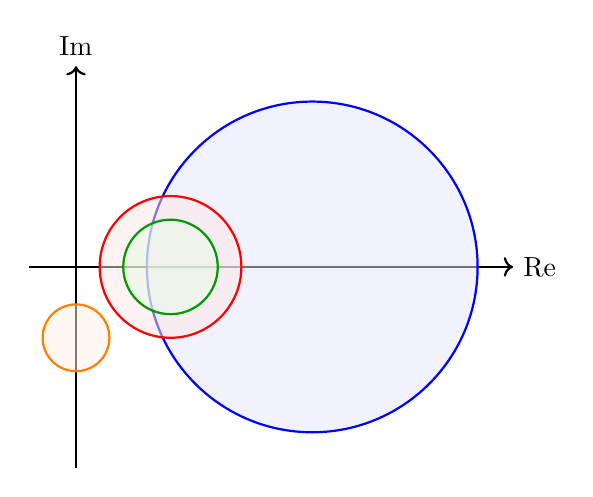
\begin{tikzpicture}[scale=0.3]
                    \draw[->, thick] (-2,0) -- (18.5,0) node[right] {Re};
                    \draw[->, thick] (0,-8.5) -- (0,8.5) node[above] {Im};

                    \draw[blue, thick, fill=blue!10, fill opacity=0.5] (10,0) circle (7);
                    \draw[red, thick, fill=red!10, fill opacity=0.5] (4,0) circle (3);
                    \draw[green!60!black, thick, fill=green!10, fill opacity=0.5] (4,0) circle (2);
                    \draw[orange, thick, fill=orange!10, fill opacity=0.5] (0,-3) circle (1.414);
                \end{tikzpicture}
            \end{center}
            \vspace{-3cm}
        \end{wrapfigure}
        Consideriamo la matrice
        \[
            \begin{pmatrix}
                10 & 1 & 3 & 3 \\
                -1 & 4 & 0 & 1 \\
                i & i & 4 & i \\
                i+1 & 0 & 0 & 3i
            \end{pmatrix}
        \]
        Abbiamo i seguenti cerchi di Gershgorin
        \begin{align*}
            C_1 &= \{ z \in \complexnumbers \suchthat |z-10| \leq 7\} \\
            C_2 &= \{ z \in \complexnumbers \suchthat |z-4| \leq 2\} \\
            C_3 &= \{ z \in \complexnumbers \suchthat |z-4| \leq 3\} \\
            C_4 &= \{ z \in \complexnumbers \suchthat |z-3i| \leq \sqrt{2}\}
        \end{align*}
        Possiamo notare che sicuramente il determinante della matrice non è nullo.
        \wrapfill
    \end{snippetexample}
\end{radioactive}

\pagebreak

\begin{snippetdefinition}{Grafo fortemente connesso}
    \todo
\end{snippetdefinition}

\subsection{Irriducibilità e grafi associati}

\begin{snippetdefinition}{Matrice irriducibile}
    Sia \(A \in \matrices_{n \times n}(\complexnumbers)\).
    Si dice che \(A\) è \emph{irriducibile}
    se \(G_A\) è fortemente connesso dove \(G_A\)
    è il grafo \((N, E)\) con \(N = \{1, \cdots, n\}\)
    dove \((J,K) \in E\) se e solo se \(A_{j,k} \neq 0\).
\end{snippetdefinition}

\begin{radioactive}
    \begin{snippetexample}{Teorema di Gershgorin II e III}
        \begin{wrapfigure}{r}{8cm}
            \begin{center}
                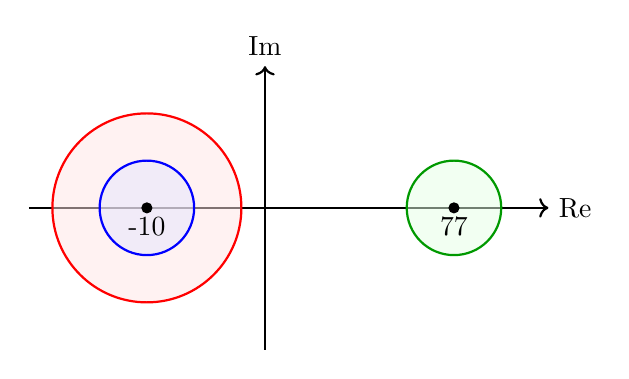
\begin{tikzpicture}[scale=0.6]
                    \draw[->, thick] (-5,0) -- (6,0) node[right] {Re};
                    \draw[->, thick] (0,-3) -- (0,3) node[above] {Im};

                    \draw[red, thick, fill=red!10, fill opacity=0.5] (-2.5,0) circle (2);
                    \draw[blue, thick, fill=blue!10, fill opacity=0.5] (-2.5,0) circle (1);

                    \draw[green!60!black, thick, fill=green!10, fill opacity=0.5] (4,0) circle (1);

                    \filldraw[black] (-2.5,0) circle (3pt) node[below] {-10};
                    \filldraw[black] (4,0) circle (3pt) node[below] {77};
                \end{tikzpicture}
            \end{center}
            \vspace{-3cm}
        \end{wrapfigure}
        Consideriamo la matrice \[
            A =
            \begin{pmatrix}
                -10 & 1   &     &     &                &    \\
                1   & -10 & 1   &     & \text{\huge 0} &    \\
                & 1   & -10 & 1   &                &    \\
                &     & 1   & -10 & 1              &    \\
                & \text{\huge 0} && 1        & -10 & 1  \\
                &     &     &     & -1             & 77
            \end{pmatrix}
        \]
        Mostrare che esiste un autovalore \(\lambda\) di questa matrice tale che
        \(\lambda = \rho(A)\). \\
        Abbiamo i cerchi
        \begin{align*}
            C_1 &= \{ z \in \complexnumbers \suchthat |z+10| \leq 1\} \\
            C_2 = C_3 = C_4 = C_5 &= \{ z \in \complexnumbers \suchthat |z+10| \leq 2\} \\
            C_6 &= \{ z \in \complexnumbers \suchthat |z-77| \leq 1\}
        \end{align*}
        C'è quindi un singolo autovalore in \(C_6\),
        ma quest'ultimo non può essere propriamente complesso in quanto ci sarebbe un'altro
        autovalore coniugato nello stesso cerchio.
        Quindi quell'autovalore è reale e coincide con il raggio spettrale, data la sua distanza dall'origine.
        Il suo grafo associato è fortemente connesso:
        \begin{center}
            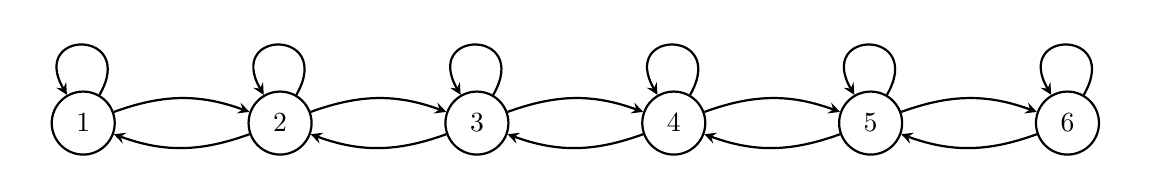
\begin{tikzpicture}[>=stealth, node distance=2cm]
                \node[circle, draw, thick, minimum size=8mm] (1) at (0,0) {1};
                \node[circle, draw, thick, minimum size=8mm] (2) at (2.5,0) {2};
                \node[circle, draw, thick, minimum size=8mm] (3) at (5,0) {3};
                \node[circle, draw, thick, minimum size=8mm] (4) at (7.5,0) {4};
                \node[circle, draw, thick, minimum size=8mm] (5) at (10,0) {5};
                \node[circle, draw, thick, minimum size=8mm] (6) at (12.5,0) {6};

                \foreach \i in {1,2,3,4,5,6} {
                    \draw[->, thick] (\i) to[out=60, in=120, looseness=6] (\i);
                }

                \foreach \i/\j in {1/2, 2/3, 3/4, 4/5, 5/6} {
                    \draw[->, thick] (\i) to[bend left=20] (\j);
                    \draw[->, thick] (\j) to[bend left=20] (\i);
                }
            \end{tikzpicture}
        \end{center}
        \wrapfill
    \end{snippetexample}
\end{radioactive}

\begin{snippettheorem}{Teorema di Gershgorin III}
    Sia \(A \in \matrices_{n \times n}(\complexnumbers)\),
    \(A\) irriducibile e tale
    l'autovalore \(\lambda\) sta sul bordo dell'unione dei cerchi
    \[
        \lambda \in \partial \left(\bigcup_{j=1}^n C_j\right)
    \]
    Allora \(\lambda\) sta sul bordo di tutti i cerchi
    \(\lambda \in \partial C_j, \forall J \in \{1, \cdots, n\}\).
\end{snippettheorem}

Non si verifica quasi mai l'ipotesi, quindi conviene usare la contronominale.

\begin{snippetproof}{Teorema di Gershgorin III}
    Sia \(\lambda\) un autovalore e sia \(x\) un suo autovettore.
    Consideriamo la relazione
    \[
        \sum_{k=1}^n A_{j,k} x_k = \lambda x_j
    \]
    dove scegliamo \(j\) come indice \(p\) tale che \(|x_p| = ||x||_\infty > 0\),
    cioè vogliamo massimizzare la parte destra.
    \begin{align*}
        \lambda x_p - A_{p,p} x_p &\leq
        \sum_{\substack{k=1 \\ k \neq p}}^n |A_{p,k}| \cdot |x_k| \leq |x_p| \cdot r_p \\
        \lambda x_p - A_{p,p} x_p &=
        \sum_{\substack{k=1 \\ k \neq p}}^n |A_{p,k}| \cdot |x_k| = |x_p| \cdot r_p
    \end{align*}
    Ma per l'ipotesi l'autovalore sta sul bordo, quindi \(r_p\) è precisamente il raggio
    del cerchio.
    Scelgo \(u = p\) e guardiamo con attenzione alla relazione
    \begin{align*}
        \sum_{\substack{k=1 \\ k \neq p}}
        |A_{p,k}| \cdot |x_k| &= \left(
            \sum_{\substack{u=1 \\ p \neq p}} |A_{p,k}|
        \right) |x_p|
    \end{align*}
    Visto che è irriducibile, almeno un termine \(i_2 \neq p\)
    esiste tale che \(A_{p,i_2} \neq 0\).
    Abbiamo quindi necessariamente che \(|x_{i_2}| = |x_p|\).
    Ma allora, tornando a Gershgorin I, avremmo potuto seguire la medesima dimostrazione
    su \(i_2 \neq p\) al posto di \(p\).
    Quindi, \(\lambda \in C_{i_2}\), e per ipotesi
    \(\lambda\) sta quindi in \(\partial C_{i_2}\).
    Iterando questo argomento \(n-1\), esaurendo l'insieme dei nodi, otteniamo la tesi.
\end{snippetproof}

\begin{snippetexample}{Teorema di Gershgorin III}
    Consideriamo la matrice
    \[
        A =
        \begin{pmatrix}
            0 & 1   &     &     &                &    \\
            & 0 & 1   &     & \text{\huge 0} &    \\
            &    & \ddots & \ddots   &                &    \\
            &     &    & \ddots & \ddots              &    \\
            & \text{\huge 0} &&         & 0 & 1  \\
            1    &     &     &     &              & 0
        \end{pmatrix}
    \]
    Ha autovalori pari a
    \[
        \lambda_j = e^{i \frac{2\pi j}{n}}
    \]
    e autovettori relativi
    \[
        v^{(j)} = \left(
            \frac{1}{\sqrt{n}} e^{i\frac{2\pi j}{n}k}
        \right)_{k=1}^n
    \]
    Il suo grafo associato è fortemente connesso: \\
    \begin{center}
        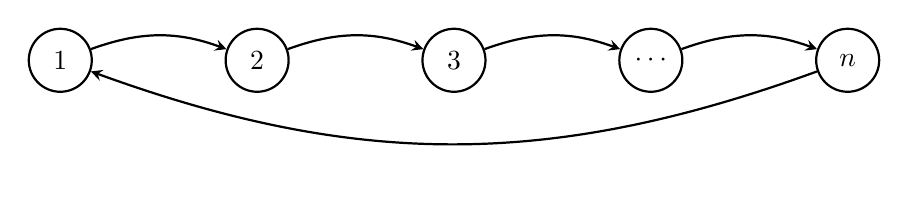
\begin{tikzpicture}[>=stealth, node distance=2cm]
            \node[circle, draw, thick, minimum size=8mm] (1) at (0,0) {1};
            \node[circle, draw, thick, minimum size=8mm] (2) at (2.5,0) {2};
            \node[circle, draw, thick, minimum size=8mm] (3) at (5,0) {3};
            \node[circle, draw, thick, minimum size=8mm] (4) at (7.5,0) {\(\cdots\)};
            \node[circle, draw, thick, minimum size=8mm] (5) at (10,0) {\(n\)};

            \foreach \i/\j in {1/2, 2/3, 3/4, 4/5} {
                \draw[->, thick] (\i) to[bend left=20] (\j);
            }

            \draw[->, thick] (5) to[bend left=20] (1);
        \end{tikzpicture}
    \end{center}
\end{snippetexample}

\pagebreak

%todo spiegazione aggiuntiva sugli esempi
\begin{snippetexample}{Teorema di Gershgorin III}
    Consideriamo la matrice
    \[
        A =
        \begin{pmatrix}
            2 & -1   &     &     &                &    \\
            -1   & 2 & -1   &     & \text{\huge 0} &    \\
            &   \ddots & \ddots & \ddots   &                &    \\
            &     &  \ddots  & \ddots & \ddots              &    \\
            & \text{\huge 0} &&       -1  & 2 & -1  \\
            &     &     &     &            -1  & 2
        \end{pmatrix}
    \]
    che discretizza l'equazione differenziale
    \[
        \begin{cases}
            -u''(x) = f(x), \quad x \in (0,1) \\
            u(0) = \alpha \\
            u(1) = \beta \\
        \end{cases}
    \]
    con \(A_n u = v\).
    Cominciamo notando che \(A_n\) è simmetrica, reale quindi Hermitiana,
    allora i suoi autovalori sono reali.
    Abbiamo i cerchi
    \begin{align*}
        C_1 &= C_n = \{ z \in \complexnumbers \suchthat |z-2| \leq 1\} \\
        C_2 = C_3 = \cdots = C_{n-1} &= \{ z \in \complexnumbers \suchthat |z-2| \leq 2\}
    \end{align*}
    \begin{wrapfigure}{r}{8cm}
        \begin{center}
            \vspace{1cm}
            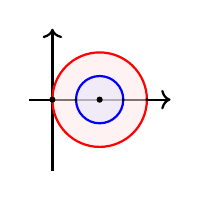
\begin{tikzpicture}[scale=0.3]
                \draw[->, thick] (-1,0) -- (5,0);
                \draw[->, thick] (0,-3) -- (0,3);

                \draw[red, thick, fill=red!10, fill opacity=0.5] (2,0) circle (2);

                \draw[blue, thick, fill=blue!10, fill opacity=0.5] (2,0) circle (1);

                \filldraw[black] (2,0) circle (3pt);
                \filldraw[black] (0,0) circle (3pt);
                \draw[dashed] (1,0) circle (1pt);
                \draw[dashed] (3,0) circle (1pt);
                \draw[dashed] (4,0) circle (1pt);

            \end{tikzpicture}
        \end{center}
        \vspace{-3cm}
    \end{wrapfigure}
    Dai teoremi di Gershgorin, siccome gli autovalori sono reali,
    sappiamo quindi che \(\lambda \in [0,4]\).
    La matrice associata è irriducibile in quanto tridiagonale.
    Tuttavia, \(0,4 \notin \partial C_1\), mentre
    \[
        0,4 \in \partial \left(
            \bigcup_{j=2}^n C_j
        \right)
    \]
    dunque \(\lambda \in (0,4)\).
    Sappiamo che se \(B = A^*\), allora \[
        \lambda_{\text{min}}(B)
        = \min_{\substack{x \in \complexnumbers^n \\ x \neq 0}} \frac{x^* B x}{x^* x}
    \]
    Ci aspettiamo che \(r_n\) sia piccolo con \(e\) il vettore di \(1\)
    \[
        A_n e =
        \begin{pmatrix} 1 & 0 & \cdots & 0 & 1
        \end{pmatrix}
    \]
    e il raggio \(r_n = 2/n \to 0\) per \(n \to \infty\).
    Se scegliessimo il vettore con elementi che si alternano \(1, -1\),
    abbiamo più sovrapposizione possibili. I coefficienti oscillano,
    il vettore oscilla e quindi risuoniamo il più possibile.
    In tal caso otteniamo un valore appena inferiore al \(4\).
    \wrapfill
\end{snippetexample}

Supponiamo che \(A \in \matrices_n(\complexnumbers)\) con \(n\) grande.
Come facciamo a verificare in maniera algoritmica se la matrice è fortemente connessa?
Sia \(G_A\) il suo grafo associato.
Consideriamo \(X\) la matrice di adiacenza di \(G_A\).
Consideriamo \(Y=X^2\), cioè
\[
    (Y)_{j,k} = \sum_{l=1}^n x_{j,l} x_{l,k}
\]
Cioè visto che i termini sono booleani, allora fa \(1\)
se posso muovermi da \(j\) a \(e\) e da \(e\) a \(k\),
quindi muoversi fra \(j\) a \(k\) in due passi.
Quindi il termine \((Y)_{j,k}\) è il numero di modi di attraversare i due nodi in \(2\) passi.
Possiamo semplificare usando una or iterata
\[
    (Y)_{j,k}
    = \bigvee_{l=1}^n x_{j,e} \cdot x_{e,k}
\]
In generale, \((X^n)_{j,k}\) ci mostra il numero di cammini
per connettere i nodi \(j, k\).
Sia \[
    \tilde X = I_n \vee \bigvee_{k=1}^{n-1} X^k
\]
Se tale matrice è tutta piena di \(1\),
significa che \(X\) è fortemente connessa.
L'identità serve per assicurarci che abbiamo uni sulla diagonale, cioè ogni elemento
ha un percorso verso sé stesso, cioè il percorso nullo.

Tuttavia, l'algoritmo più ottimale è quello
di fare un traversamento DFS sul grafo, controllare, e poi un traversamente DFS
sul grafo invertito (che è associato alla matrice trasposta).

\subsection{Applicazioni ai metodi iterativi}

\begin{snippetexample}{Jacobi e Gauss-Seidel su una matrice non a predominanza diagonale}
    Sia \(N>100\). Per \(j=1,\ldots,N-2\) poniamo
    \[
        b_j = 1-\frac{1}{j+1},
        \qquad
        a_j = \frac{1}{2}\left(b_j+\frac{1}{b_j}\right).
    \]
    Allora \(b_j>0\), \(b_j \to 1\), \(a_j>0\) e \(a_j \to 1\). Consideriamo la matrice
    \[
        Q =
        \begin{pmatrix}
            a_1 & 1 & \cdots & 1 \\
            1 & a_2 & \cdots & 1 \\
            \vdots & \vdots & \ddots & \vdots \\
            1 & 1 & \cdots & a_{N-2}
        \end{pmatrix}.
    \]
    La matrice \(Q\) non è a predominanza diagonale. Vogliamo risolvere il sistema
    \[
        Qx=b,
        \qquad
        x^\ast =
        \begin{pmatrix}
            1 \\
            \vdots \\
            1
        \end{pmatrix},
        \qquad
        b=Qx^\ast.
    \]

    Per il metodo di Jacobi si considera lo splitting
    \[
        M=D=\operatorname{diag}(a_j),
        \qquad
        N=B+C,
        \qquad
        N_{ij} =
        \begin{cases}
            -1 & \text{se } i\neq j,\\
            0 & \text{se } i=j.
        \end{cases}
    \]
    Quindi l'iterazione è
    \[
        x_i^{(k+1)}
        =
        \frac{1}{a_i}
        \left(
            b_i-\sum_{\substack{j=1\\ j\neq i}}^{N-2}x_j^{(k)}
        \right).
    \]
    La matrice di iterazione di Jacobi è
    \[
        J=D^{-1}(B+C),
        \qquad
        \rho(J)>10.
    \]
    Dunque Jacobi non converge.

    Per Gauss-Seidel si considera invece
    \[
        M=D-B=\operatorname{tril}(Q),
    \]
    e in questo caso la matrice di iterazione \(G\) soddisfa
    \[
        \rho(G)<1.
    \]
    Quindi Gauss-Seidel converge.
\end{snippetexample}

\subsection{Convergenza, consistenza e stabilità}

\begin{snippettheorem}{Convergenza, consistenza e stabilità}
    Sia \(\mathcal{A}\) un metodo iterativo della forma
    \[
        x^{(k+1)} = Px^{(k)}+q.
    \]
    Allora \(\mathcal{A}\) è convergente se e solo se \(\mathcal{A}\) è consistente e stabile, cioè se e solo se
    \[
        x^\ast = Px^\ast+q
        \qquad\text{e}\qquad
        \rho(P)<1.
    \]
\end{snippettheorem}

\begin{snippetproof}{}
    Dimostriamo le due implicazioni separatamente.

    \begin{iffproof}
    \item Supponiamo che il metodo sia convergente. Per ipotesi, per ogni dato iniziale
        \(x^{(0)}\in\complexnumbers^n\), la successione \(\{x^{(k)}\}_{k\geq 0}\) converge alla soluzione
        \(x^\ast\). Passando al limite nell'iterazione otteniamo
        \[
            x^\ast
            =
            \lim_{k\to+\infty}x^{(k+1)}
            =
            \lim_{k\to+\infty}\left(Px^{(k)}+q\right)
            =
            Px^\ast+q.
        \]
        Dunque il metodo è consistente.

        Mostriamo ora che è stabile. Supponiamo per assurdo che non lo sia. Allora
        \[
            \rho(P)\geq 1.
        \]
        Quindi esiste un autovalore \(\widehat{\lambda}\in\sigma(P)\) tale che
        \[
            |\widehat{\lambda}|\geq 1.
        \]
        Sia \(\widehat{u}\neq 0\) un autovettore relativo a \(\widehat{\lambda}\), cioè
        \[
            P\widehat{u}=\widehat{\lambda}\widehat{u}.
        \]
        Prendiamo come dato iniziale
        \[
            \widehat{x}^{(0)}=x^\ast+\widehat{u}
        \]
        e consideriamo la successione \(\{\widehat{x}^{(k)}\}_{k\geq 0}\) generata dal metodo. Definiamo
        \[
            \widehat{e}^{(k)}=\widehat{x}^{(k)}-x^\ast.
        \]
        Poiché il metodo è consistente,
        \[
            x^\ast=Px^\ast+q,
            \qquad
            \widehat{x}^{(k+1)}=P\widehat{x}^{(k)}+q.
        \]
        Sottraendo le due identità si ottiene l'equazione dell'errore
        \[
            \widehat{e}^{(k+1)}=P\widehat{e}^{(k)}.
        \]
        Quindi
        \[
            \widehat{e}^{(k)}
            =
            P^k\widehat{e}^{(0)}.
        \]
        Ma
        \[
            \widehat{e}^{(0)}
            =
            \widehat{x}^{(0)}-x^\ast
            =
            \widehat{u}.
        \]
        Essendo \(\widehat{u}\) autovettore di \(P\), segue che
        \[
            \widehat{e}^{(k)}
            =
            P^k\widehat{u}
            =
            \widehat{\lambda}^k\widehat{u}.
        \]
        In particolare,
        \[
            \norm{\widehat{e}^{(k)}}_\infty
            =
            {|\widehat{\lambda}|}^k\norm{\widehat{u}}_\infty
            \geq
            \norm{\widehat{u}}_\infty
            \neq 0.
        \]
        Quindi \(\widehat{x}^{(k)}\) non converge a \(x^\ast\), contro l'ipotesi di convergenza del metodo.
        Ne segue che necessariamente \(\rho(P)<1\).

    \item Supponiamo ora che il metodo sia consistente e stabile. Vogliamo mostrare che per ogni
        \(x^{(0)}\in\complexnumbers^n\) la successione \(\{x^{(k)}\}_{k\geq 0}\), definita da
        \[
            x^{(k+1)}=Px^{(k)}+q,
        \]
        converge a \(x^\ast\), soluzione del sistema \(Ax=b\).

        Per consistenza vale
        \[
            x^\ast=Px^\ast+q.
        \]
        Sottraendo questa identità dall'iterazione,
        \[
            x^{(k+1)}-x^\ast
            =
            P\left(x^{(k)}-x^\ast\right).
        \]
        Definendo
        \[
            e^{(k)}=x^{(k)}-x^\ast,
        \]
        otteniamo
        \[
            e^{(k+1)}=Pe^{(k)}.
        \]
        Per induzione,
        \[
            e^{(k)}=P^k e^{(0)}.
        \]
        Poiché il metodo è stabile, \(\rho(P)<1\). Quindi
        \[
            P^k\to 0
            \qquad\text{in }\complexnumbers^{n\times n}.
        \]
        Di conseguenza
        \[
            e^{(k)}=P^k e^{(0)}\to 0,
        \]
        e dunque
        \[
            x^{(k)}\to x^\ast.
        \]
    \end{iffproof}
\end{snippetproof}

\section{Analisi dell'errore nei metodi iterativi}

\subsection{Tassi di riduzione dell'errore}

Il raggio spettrale \(\rho(P)\) fornisce asintoticamente il tasso di riduzione dell'errore. Se
\[
    \norm{e^{(k)}}=\gamma_k\norm{e^{(k-1)}},
\]
allora
\[
    \gamma_k
    =
    \frac{\norm{e^{(k)}}}{\norm{e^{(k-1)}}}.
\]

\begin{snippetdefinition}{Tasso di riduzione medio dell'errore}
    Il \emph{tasso di riduzione medio dell'errore} al passo \(k\) è
    \[
        t_k
        =
        \sup_{e^{(0)}\in\complexnumbers^n}
        \sqrt[k]{
            \prod_{j=1}^k
            \frac{\norm{e^{(j)}}}{\norm{e^{(j-1)}}}
        }
        =
        \sup_{e^{(0)}\in\complexnumbers^n}
        \sqrt[k]{
            \frac{\norm{e^{(k)}}}{\norm{e^{(0)}}}
        }.
    \]
\end{snippetdefinition}

\begin{snippettheorem}{}
    Si ha
    \[
        \lim_{k\to+\infty}t_k=\rho(P).
    \]
\end{snippettheorem}

\begin{snippetproof}{}
    Osserviamo innanzitutto che
    \[
        e^{(k)}=P^k e^{(0)}.
    \]
    Quindi
    \[
        t_k^k
        =
        \sup_{e^{(0)}\in\complexnumbers^n}
        \frac{\norm{P^k e^{(0)}}}{\norm{e^{(0)}}}
        =
        \norm{P^k}.
    \]
    Perciò
    \[
        t_k=\sqrt[k]{\norm{P^k}}.
    \]
    La conclusione segue dalla formula di Gelfand:
    \[
        \lim_{k\to+\infty}\sqrt[k]{\norm{P^k}}=\rho(P).
    \]

    Per completezza, ricordiamo anche l'idea della stima. Sia \(\lambda\in\sigma(P)\) tale che
    \[
        |\lambda|=\rho(P),
    \]
    e sia \(u\neq 0\) un autovettore relativo a \(\lambda\), con \(\norm{u}=1\). Prendendo
    \(e^{(0)}=u\), si ha
    \[
        \norm{e^{(k)}}
        =
        \norm{P^k u}
        =
        \norm{\lambda^k u}
        =
        {|\lambda|}^k.
    \]
    Quindi
    \[
        t_k
        \geq
        \sqrt[k]{\frac{\norm{e^{(k)}}}{\norm{u}}}
        =
        |\lambda|
        =
        \rho(P).
    \]
    D'altra parte, per ogni \(\varepsilon>0\) esiste una norma matriciale indotta tale che
    \[
        \norm{P}\leq \rho(P)+\varepsilon.
    \]
    Allora
    \[
        t_k^k
        =
        \norm{P^k}
        \leq
        \norm{P}^k
        \leq
        \left(\rho(P)+\varepsilon\right)^k,
    \]
    e dunque
    \[
        t_k\leq \rho(P)+\varepsilon.
    \]
    Facendo tendere \(\varepsilon\) a \(0\), otteniamo
    \[
        \lim_{k\to+\infty}t_k=\rho(P).
    \]
\end{snippetproof}

\begin{snippettheorem}{}
    Se il metodo è convergente e l'errore non si annulla, allora
    \[
        \gamma_k
        =
        \frac{\norm{e^{(k)}}}{\norm{e^{(k-1)}}}
        \to
        \rho(P)
        \qquad
        \text{per } k\to+\infty.
    \]
\end{snippettheorem}

\begin{snippetproposition}{Osservazione}
    Se \(\rho(P)=\frac{1}{2}\), asintoticamente ci aspettiamo
    \[
        \norm{e^{(k)}}
        \approx
        \frac{1}{2}\norm{e^{(k-1)}}.
    \]
\end{snippetproposition}

\begin{snippetproposition}{Osservazione}
    Il raggio spettrale \(\rho(P)\) determina la velocità di convergenza del metodo iterativo. Se vogliamo
    \(q\) cifre di precisione nella soluzione, dobbiamo imporre
    \[
        \frac{\norm{e^{(k)}}}{\norm{e^{(0)}}}<10^{-q}.
    \]
    Usando l'approssimazione asintotica
    \[
        \frac{\norm{e^{(k)}}}{\norm{e^{(0)}}}
        \approx
        \rho(P)^k,
    \]
    richiediamo
    \[
        10^{-q}>\rho(P)^k.
    \]
    Passando al logaritmo in base \(10\), siccome \(0<\rho(P)<1\), otteniamo
    \[
        -q>k\log_{10}\rho(P),
    \]
    e quindi
    \[
        k>
        -\frac{q}{\log_{10}\rho(P)}
        >0.
    \]
    Ad esempio, confrontare i casi \(\rho(P)=0.79\) e \(\rho(P)=0.83\): anche una piccola variazione del
    raggio spettrale può aumentare sensibilmente il numero di iterazioni necessarie.
\end{snippetproposition}

Il valore \(t_k\) è una stima asintotica a priori, ma per usarla bisogna conoscere \(\rho(P)\), oppure almeno
una sua stima. Un'alternativa è definire criteri d'arresto differenti.

I due criteri più comuni sono:
\[
    \frac{\norm{r^{(k)}}}{\norm{b}}<\varepsilon,
    \qquad
    r^{(k)}=b-Ax^{(k)},
\]
dove \(r^{(k)}\) è il \emph{residuo} del metodo iterativo al passo \(k\), oppure
\[
    \frac{\norm{x^{(k)}-x^{(k-1)}}}{\norm{x^{(k)}}}<\varepsilon.
\]
Il secondo criterio è sconsigliato quando il raggio spettrale è troppo vicino a \(1\).

\subsection{Criteri d'arresto}

Vogliamo capire cosa succede quando fermiamo il metodo con i criteri precedenti. Definiamo l'\emph{errore relativo}
come
\[
    \frac{\norm{e^{(k)}}}{\norm{x^\ast}}
    =
    \frac{\norm{x^\ast-x^{(k)}}}{\norm{x^\ast}}.
\]

\subsubsection{Criterio basato sul residuo}

Poiché \(Ax^\ast=b\), si ha
\begin{align*}
    r^{(k)}
    &= b-Ax^{(k)} \\
    &= Ax^\ast-Ax^{(k)} \\
    &= A\left(x^\ast-x^{(k)}\right) \\
    &= Ae^{(k)}.
\end{align*}
Quindi
\[
    e^{(k)}=A^{-1}r^{(k)}.
\]
Pertanto
\[
    \norm{e^{(k)}}
    \leq
    \norm{A^{-1}}\norm{r^{(k)}}.
\]
Inoltre
\[
    b=Ax^\ast
    \qquad\Longrightarrow\qquad
    \norm{b}
    =
    \norm{Ax^\ast}
    \leq
    \norm{A}\norm{x^\ast}.
\]
Da cui
\[
    \frac{1}{\norm{x^\ast}}
    \leq
    \frac{\norm{A}}{\norm{b}}.
\]
Allora
\begin{align*}
    \frac{\norm{e^{(k)}}}{\norm{x^\ast}}
    &\leq
    \norm{A^{-1}}\norm{r^{(k)}}\frac{\norm{A}}{\norm{b}} \\
    &=
    \norm{A^{-1}}\norm{A}\frac{\norm{r^{(k)}}}{\norm{b}}.
\end{align*}
Se il criterio d'arresto impone
\[
    \frac{\norm{r^{(k)}}}{\norm{b}}<\varepsilon,
\]
allora
\[
    \frac{\norm{e^{(k)}}}{\norm{x^\ast}}
    <
    \operatorname{cond}(A)\varepsilon.
\]
Quindi il criterio basato sul residuo controlla bene l'errore relativo quando \(\operatorname{cond}(A)\) non è troppo grande.

\subsubsection{Criterio basato sulla differenza fra iterati consecutivi}

Osserviamo che
\begin{align*}
    x^{(k)}-x^{(k-1)}
    &=
    x^{(k)}-x^\ast+x^\ast-x^{(k-1)} \\
    &=
    -e^{(k)}+e^{(k-1)} \\
    &=
    -Pe^{(k-1)}+e^{(k-1)} \\
    &=
    (I-P)e^{(k-1)}.
\end{align*}
Poiché \(\rho(P)<1\), la matrice \(I-P\) è invertibile. Quindi
\[
    e^{(k-1)}
    =
    (I-P)^{-1}\left(x^{(k)}-x^{(k-1)}\right).
\]
Di conseguenza,
\[
    \frac{\norm{e^{(k-1)}}}{\norm{x^{(k)}}}
    \leq
    \norm{(I-P)^{-1}}
    \frac{\norm{x^{(k)}-x^{(k-1)}}}{\norm{x^{(k)}}}.
\]
Se il criterio d'arresto impone
\[
    \frac{\norm{x^{(k)}-x^{(k-1)}}}{\norm{x^{(k)}}}<\varepsilon,
\]
allora
\[
    \frac{\norm{e^{(k-1)}}}{\norm{x^{(k)}}}
    \leq
    \norm{(I-P)^{-1}}\varepsilon.
\]
Questo criterio può essere poco affidabile quando \(\rho(P)\approx 1\): in quel caso \(I-P\) è vicina a essere
singolare e quindi \(\norm{(I-P)^{-1}}\) può essere molto grande. In altre parole, gli iterati consecutivi possono
essere molto vicini anche se l'errore rispetto alla soluzione è ancora grande.

\subsection{Gauss-Seidel per matrici Hermitiane definite positive}

\begin{snippettheorem}{}
    Sia \(A\) Hermitiana con elementi principali reali positivi,
    cioè \(a_{i,i} > 0\).
    Allora, l'iterazione di Gauss-Seidel è convergente se e solo se \(A\) è definita positiva.
\end{snippettheorem}

\begin{snippetproof}{}
    Decomponiamo la matrice come \(A = D - B - C = D - B - B^H\)
    siccome è Hermitiana.
    Allora la matrice di iterazione è
    \begin{align*}
        G &= (D-B)^{-1}C
        = (D- B)^{-1} B^H \\
        &= (D-B)^{-1}(B^H + D - B - D + D) = I - (D - B)^{-1}A
    \end{align*}
    Prima di dimostrare l'uguaglianza, mostriamo
    che la matrice \(Z \triangleq A-G^H A G\) è definita positiva.
    Poniamo \(F \triangleq (D-B)^{-1}A\).
    Data l'uguaglianza precedente \(G = I-F\).
    In particolare,
    \begin{align*}
        Z &= A- G^HAG = A - (I-F)^H A (I - F) \\
        &= \cancel A - \cancel A + F^H A + AF - FAF
        = F^H\left(A + F^{-H}AF - AF\right) \\
        &= F^H \left(AF^{-1} + F^{-H}A - A\right)F \\
        &= F^H \left(
            \cancel{AA^{-1}}(D-B) + (D-B)^H \cancel{A^{-H}A} - A
        \right)F \\
        &= F^H \left(
            D-B+D - B^H - A
        \right)F = F^H(D + A - A)F
        = F^H D F
    \end{align*}
    \(F\) è non singolare perché \((D-B)^{-1}\) e \(A\) non lo sono nemmeno.
    Inoltre, siccome \(A\) ha elementi principali positivi, \(D\) a sua volta ha elementi
    reali positivi, quindi \(\forall x \in \complexnumbers^n \difference \{0\}\)
    \begin{DispWithArrows*}
        x^H Z x &= x^H(A - G^HAG)x= x^HF^HDFx  \Arrow{\(y=Fx\)} \\
        &= y^H D y = \sum_{i=1}^n A_{i,i} \underbrace{|y_i|^2}_{\geq 0} > 0
    \end{DispWithArrows*}
    Concludiamo ora il teorema:
    \begin{ffiproof}
    \item Supponiamo che \(A\) sia definita positiva.
        Consideriamo un autovalore \(\lambda \in \sigma(G)\) e \(x\)
        autovettore corrispondente, quindi \(Gx = \lambda x\).
        Siccome \(A\) è definita positiva,
        \begin{align*}
            x^H Z x &= x^H(A- G^H A G)x = x^H Ax - x^H G^H A G x \\
            &= x^H A x - \overline{\lambda} x^H A \lambda x = x^H A x - |\lambda|^2 x^H Ax \\
            &= \left(1 - |\lambda|^2\right)x^H A x
        \end{align*}
        Siccome \(Z\) è definito positivo,
        questo termine è positivo se e solo se \(1-|\lambda|^2\),
        cioè \(1 > |\lambda|\).
        In altre parole se e solo se \(\rho(G) < 1\).
    \item Supponiamo che il metodo sia convergente e mostriamo che \(A\)
        è definita positiva. Consideriamo l'errore \[
            e^{(k)} = x^\ast - x^{(k)}
        \]
        dove \(x^\ast\) è la soluzione del sistema.
        Questa successione tende a zero per ipotesi.
        Poiché \(e^{(k)} = Pe^{(k-1)}, \forall k \geq 1\), abbiamo
        \(e^{(k)} = Ge^{(k-1)}\). Allora, considerando la matrice \(Z\) dello scorso punto,
        \begin{align*}
            x^H Z x &= (e^{(0)})^H A e^{(0)}
            - \frac{
                (e^{(0)})^H G^H A \overbrace{Ge^{(0)}}^{(e^{(1)})}
            }{
                (e^{(1)})^H
            } = (e^{(0)})^H A e^{(0)} - (e^{(1)})^H A (e^{(1)})
        \end{align*}
        O più in generale
        \[
            0 < (e^{(k)})^H Z e^{(k)}
            = \underbrace{(e^{(k)})^H A e^{(k)}}_{\alpha_n}
            - \underbrace{(e^{(k+1)})^H A e^{(k+1)}}_{\alpha_{n+1}}
            \iff \alpha_n > \alpha_{n+1}
        \]
        cioè se la successione tende a zero dal basso.
        Supponiamo per assurdo che \(A\) non sia definita positiva, allora esisterebbe
        un certo vettore \(e_0 \neq 0\) (cioè un errore iniziale particolare)
        per cui
        \begin{align*}
            (e^{(0)})^H A e^{(0)} \leq 0
        \end{align*}
        e quindi la successione non tende a zero dall'alto, il che è assurdo perché per ipotesi il metodo converge.
    \end{ffiproof}
\end{snippetproof}

\subsection{Metodi di rilassamento}

Metodo di rilassamento:
se lo spettro della matrice è troppo vicno ad uno, esiste una modifica che sposta
lo spettro più in basso per acellerare la convergenza. Al posto di risolvere \(Ax = b\)
risolviamo \(\omega Ax = \omega b\).
Una volta effettuata la decomposizione \(\omega A = M - N\)
vale
\(M = D-\omega B\) e \(N = (1-\omega) D + \omega C\).
Se il determinante di \(N\) è non nullo, \[
    x^{(k)} = \underbrace{(D-\omega B)^{-1} \left[
            (1-\omega) D + \omega C
    \right]}_{P_\omega}
    x^{(k-1)} + \omega(D - \omega B)^{-1}b
\]
A questo punto abbiamo due classi di rilassamento, quelli \(\omega > 1\) (sovrarilassamenti)
e \(\omega < 1\) (sottorilassamenti).
Abbiamo \(\rho(P_\omega) > |\omega-1|\),
quindi se \(|\omega-1| \geq 1\) non convergerà.

\subsection{Esempi di confronto fra Jacobi e Gauss-Seidel}

\begin{snippetexample}{}
    Consideriamo la matrice
    \[
        A =
        \begin{pmatrix}
            -4 & -1 & 1 & 1 \\
            0 & -4 & -1 & 1 \\
            -1 & -1 & 4 & 1 \\
            1 & -1 & 0 & 4
        \end{pmatrix}
    \]
    ha predominanza diagonale forte.
    Abbiamo le matrici di Jacobi e Gauss-Seidel \[
        J = \frac14
        \begin{pmatrix}
            0 & -1 & 1 & 1 \\
            0 & 0 & -1 & 1 \\
            1 & 1 & 0 & -1 \\
            -1 & 1 & 0 & 0
        \end{pmatrix},
        \quad
        G = \frac{1}{16}
        \begin{pmatrix}
            0 & -4 & 4 & 4 \\
            0 & 0 & -4 & 4 \\
            0 & -1 & 0 & -2 \\
            0 & 1 & -2 & 0
        \end{pmatrix}
    \]
    Il polinomio caratteristiche della matrice di Gauss-Seidel è
    \begin{align*}
        \rho_G(\lambda)
        &= -\lambda^4 - \frac{3}{64}\lambda^2
        - \frac{\lambda}{256} = \lambda\left(\lambda - \frac14\right)
        \left(\lambda + \frac18\right)^2
    \end{align*}
    Abbiamo quindi autovalore \(\lambda = 0, \frac14, -\frac18, -\frac18\)
    e il raggio spettrale è minore di \(1\), quindi converge.
    Lo spettro della matrice di Jacobi è
    \begin{align*}
        \lambda_1 = \lambda_2 = \frac14, \quad
        \lambda_3 = \frac{-1 + i\sqrt{2}}{4},
        \lambda_4 = \frac{-1 - i\sqrt{2}}{4}
    \end{align*}
    il raggio spettrale è \(\sfrac{\sqrt{3}}{4} < 1\), quindi il metodo è convergente.
\end{snippetexample}

\begin{snippetexample}{}
    Consideriamo la matrice
    \[
        A =
        \begin{pmatrix}
            -4 & -1 & 1 & 1 \\
            0 & -4 & -1 & -3 \\
            -1 & -1 & 4 & 1 \\
            1 & 3 & 0 & 4
        \end{pmatrix}
    \]
    ha predominanza diagonale debole ed è irridubicile.
    Abbiamo le matrici di Jacobi e Gauss-Seidel \[
        J = \frac14
        \begin{pmatrix}
            0 & -1 & 1 & 1 \\
            0 & 0 & -1 & -3 \\
            1 & 1 & 0 & -1 \\
            -1 & -3 & 0 & 0
        \end{pmatrix},
        \quad
        G = \frac{1}{16}
        \begin{pmatrix}
            0 & -4 & 4 & 4 \\
            0 & 0 & -4 & -12 \\
            0 & -1 & 0 & -6 \\
            0 & 1 & 2 & 8
        \end{pmatrix}
    \]
    Gli spettri sono
    \[
        \sigma_J = \left\{
            \frac14, -\frac34, \frac{1 + \sqrt{2}}{4}, \frac{1-\sqrt{2}}{4}
        \right\},
        \quad
        \sigma_G = \left\{
            0, \frac14, \frac18
        \right\}
    \]
    Abbiamo ancora quindi la convergenza in ambo i metodi.
\end{snippetexample}

\begin{snippetexample}{}
    Consideriamo la matrice
    \[
        A =
        \begin{pmatrix}
            -4 & -1 & 1 & 1 \\
            0 & -4 & 0 & -4 \\
            1 & 1 & 4 & 1 \\
            0 & -4 & 0 & 4
        \end{pmatrix}
    \]
    ha predominanza diagonale debole ma non è irridubicile.
    Abbiamo le matrici di Jacobi e Gauss-Seidel \[
        J = \frac14
        \begin{pmatrix}
            0 & -1 & 1 & 1 \\
            0 & 0 & 0 & -4 \\
            -1 & -1 & 0 & -1 \\
            0 & 4 & 0 & 0
        \end{pmatrix},
        \quad
        G = \frac{1}{16}
        \begin{pmatrix}
            0 & -4 & 4 & 4 \\
            0 & 0 & 0 & -16 \\
            0 & -1 & -1 & -1 \\
            0 & 0 & 0 & 16
        \end{pmatrix}
    \]
    Il polinomio caratteristico della matrice \(J\) è
    \[
        \rho_J(\lambda) =
        \lambda^4 + \frac{17}{16}\lambda^2 + \frac{1}{16}
        = \left(\lambda^2 + 1\right)\left(\lambda^2 + 16\right)
    \]
    quindi abbiamo autovalori \(\lambda_1 = i, \lambda_2 = -i, \lambda_3 = \frac{i}{4}, \lambda_4 = -\frac{i}{4}\).
    Abbiamo quindi un raggio spettrale di esattamente \(1\), e quindi nessuna convergenza.
    Il polinomio caratteristiche per Gauss-Seidel abbimo
    \[
        \rho_J(\lambda) = \lambda^4 + \frac{17}{16}\lambda^3 + \frac{\lambda^2}{16}
        = \lambda^2\left(\lambda + 1\right)\left(\lambda + \frac{1}{16}\right)
    \]
    abbiamo quindi autovalori
    \(\lambda_1 = \lambda_2 = 0, \lambda_3 = -1, \lambda_4 = -\frac{1}{16}\),
    quindi ancora una volta abbiamo il raggio spettrale pari a \(1\).
\end{snippetexample}

\subsection{Matrici consistentemente ordinate e confronto asintotico}

\begin{snippetdefinition}{Consistentemente ordinata}
    Siano \(A \in \matrices_n(\complexnumbers)\)
    e \(\det A \neq 0\)
    con \(A = D - B - C\) e \(\det D \neq 0\).
    Scriviamo \(P_J = D^{-1}(D + B)\)
    e \(P_{GS} = (D-B)^{-1}C\).
    Per semplicità indichiamo \(P_J = L+U\)
    con \(L = D^{-1}B\)
    e \(U = D^{-1}C\), e analogamente
    \[
        P_{GS} = (D(I-D^{-1}B))^{-1}C = (I - D^{-1} B)^{-1}D^{-1}C
        = (I-L)U
    \]
    Si dice che \(A\) è \emph{consistentemente ordinata}
    se \(\forall \alpha \neq 0\) vale \(P_J\)
    è simile \[
        P_J(\alpha) \triangleq \alpha L + \frac{1}{\alpha}U
    \]
\end{snippetdefinition}

Le matrici tridiagonali che soddisfano le ipotesi della definizione sono
consistentemente ordinate. Sia infati \(A \in \matrices_n(\complexnumbers)\)
tridiagonale, allora \(B\) è nulla tranne la sottodiagonale, e \(C\)
è nulla tranne la sopradiagonale. Siccome la riscalatura
non cambia il pattern della matrice, pure \(L\) hanno queste forme rispettivamente.
\[
    L =
    \begin{pmatrix}
        0 & & && \\
        l_{2,1} & \ddots & && \\
        & l_{3,2} & \ddots && \\
        & & \ddots & \ddots & \\
        & & & l_{n,n-1} & 0
    \end{pmatrix}, \quad
    U =
    \begin{pmatrix}
        0 & u_{1,2} & && \\
        & \ddots & u_{2,3} && \\
        & &  \ddots & \ddots & \\
        & & & 0 & u_{n-1,n}
    \end{pmatrix}
\]
Consideriamo la matrice \(\Delta = \operatorname{diag}(1, \alpha, \alpha^2, \cdots, \alpha^{n-1})\)
da cui \(\Delta P_J = \Delta^{-1} = P_J(\alpha)\).
Questa matrice applicata ad ogni matrice della forma \(X = J + U\)
produce la forma \(\alpha L + \frac{1}{\alpha}U\).
Quindi, questa classe include le tridiagonali ed è abbastanza ampia da chiedersi
cosa fanno i metodi iterativi.

\begin{snippettheorem}{}
    Siano \(A \in \matrices_n(\complexnumbers)\)
    e \(\det A \neq 0\)
    con \(A = D - B - C\) e \(\det D \neq 0\).
    Scriviamo \(P_J = D^{-1}(D + B)\)
    e \(P_{GS} = (D-B)^{-1}C\).
    Per semplicità indichiamo \(P_J = L+U\)
    con \(L = D^{-1}B\)
    e \(U = D^{-1}C\), e analogamente
    \[
        P_{GS} = (D(I-D^{-1}B))^{-1}C = (I - D^{-1} B)^{-1}D^{-1}C
        = (I-L)U
    \]
    Sia \(A\) consistentemente ordinata.
    Allora, \[
        \rho\left(P_{GS}\right)
        = \rho^2(P_J)
    \]
\end{snippettheorem}

Quindi, o divergono assieme o convergono assieme, e quando convergono Gauss-Seidel
è il doppio più veloce.

\begin{snippetproof}{}
    Valutiamo il polinomio caratteristico
    \begin{DispWithArrows*}
        \det(P_{GS} - \lambda I)
        &= \det\left((I-L)^{-1}U - \lambda I\right)
        = \cancelto{1}{\det((I-L)^{-1})}
        \det(U - \lambda(I-L)) \\
        &= \det(U + \lambda L - \lambda I) \Arrow{\(\lambda \neq 0\)} \\
        &= \det\left(
            \sqrt\lambda \left(
                \sqrt\lambda L + \frac{1}{\sqrt\lambda} U - \sqrt\lambda I
            \right)
        \right) \\
        &= \left(\sqrt \lambda\right)^n
        \det \left(
            \sqrt \lambda L + \frac{1}{\sqrt \lambda} U - \sqrt \lambda I
        \right) = g(\lambda)
    \end{DispWithArrows*}
    Possiamo eliminare il caso \(\lambda \neq 0\)
    in quanto la radice nulla non contribuisce verso il raggio spettrale.
    Facciamo diventare questa funzione a due variabili, cioè \(g(\lambda) = f(\lambda, \sqrt\lambda)\)
    \begin{align*}
        f(\lambda, \mu) &= (\sqrt\lambda)^n \det\left(
            \sqrt\lambda L + \frac{1}{\sqrt\lambda}U - \mu I
        \right) \\
        &= (\sqrt\lambda)^n \operatorname{pol. char}\underbrace{\left(\sqrt\lambda L + \frac{1}{\sqrt \lambda}U\right)(\mu)}_{P_J(\sqrt\lambda) \sim P_J}(\mu)
        = (\sqrt\lambda)^n \det\left(
            P_j - \mu I
        \right)
    \end{align*}
    Quindi, purché \(\lambda\) sia autovalore nullo, che non mi interessa, allora
    per \(\lambda\) che annulla il polinomio caratteristico di Gauss-Seidel, quello
    che annulla il polinomio caratteristico di Jacobi è \(\sqrt\lambda\).
    Ciò vale per tutti gli autovalori grandi e quindi vale per il raggio spettrale.
    Quindi abbiamo inolte dimostrato che per ogni autovalore non-nullo di Gauss-Seidel
    ne corrisponde uno, la radice, per la matrice di Jacobi.
\end{snippetproof}

Questa condizione/problematicca dell'autovalore nullo è in realtà inevitabile.
Consideriamo
\[
    A =
    \begin{pmatrix}
        1 & \alpha \\ \alpha & 1
    \end{pmatrix} \in \matrices_2(\complexnumbers)
\]
con \(|\alpha|<1\). I metodi convergono
e la matrice è tridiagonale (come tutte le matrici \(2\times 2\)).
Abbiamo quindi
\[
    P_J = D^{-1}(B + C) =
    \begin{pmatrix}
        0 & -\alpha & \alpha & 0
    \end{pmatrix}
\]
Se consideriamo il vettore di tutti \(1\), troviamo che un autovalore è
per esempio \(\alpha\). Siccome la traccia è nulla l'altro autovalore è \(-\alpha\).
D'altra parte abbiamo \[
    P_{GS} = (D-B)^{-1}C =
    \begin{pmatrix}
        1 & 0 \\ \alpha 1
    \end{pmatrix}^{-1}
    \begin{pmatrix}
        0 & -\alpha \\ 0 & 0
    \end{pmatrix}
    =
    \begin{pmatrix}
        1 & 0 \\ -\alpha & 1
    \end{pmatrix}
    \begin{pmatrix}
        0 & -\alpha \\ 0 & 0
    \end{pmatrix}
    =
    \begin{pmatrix}
        0 & -\alpha \\ 0 & \alpha^2
    \end{pmatrix}
\]
Quindi a zero non corrisponde la radice di zero cioè zero come autovalore.
La matrice di Jacobi ha sempre uno autovalore nullo,
mentre quella di Gauss-Seidel non necessariamente.
Esistono matrici per cui \(J\) e \(GS\) sono ben definite tali che \(\rho(P_J) < 1\)
e \(\rho(P_{GS}) > 1\).
Esistono matrici per cui \(J\) e \(GS\) sono ben definite tale che
\(\rho(P_{GS}) < 1\) e \(\rho(P_J) > 1\).

\begin{snippetexercise}{
        Per \(M>1\) esistono matrici per cui \(J\) e \(GS\) sono ben definite tali che
        \(\rho(P_{GS}) < 1\) e \(\rho(P_J) > M\).
    }
    In questo modo, abbiamo sempre la convergenza di Gauss-Seidel in quanto la matrice è
    definita positiva, ma sufficientemente poco a predominanza diagonale da non fare
    convergere Jacobi.

    Vogliamo costruire un caso limite di una matrice definita positiva ma non troppo
    a predominanza diagonale. Consideriamo la matrice con tutti elementi uguali a \(1\)
    e aggiungiamo \(\varepsilon I\), con \(\varepsilon>0\):
    \[
        A_{n,\varepsilon}
        =
        \begin{pmatrix}
            1 & 1 & \cdots & 1 \\
            1 & 1 & \cdots & 1 \\
            \vdots & \vdots & \ddots & \vdots \\
            1 & 1 & \cdots & 1
        \end{pmatrix}
        + \varepsilon I.
    \]
    Indichiamo con \(E\) la matrice con tutti elementi uguali a \(1\). Allora
    \[
        A_{n,\varepsilon}=E+\varepsilon I.
    \]
    Questa matrice è definita positiva, infatti gli autovalori di \(E\) sono
    \[
        \lambda(E)=
        \begin{cases}
            0 & \text{con molteplicità } n-1, \\
            n & \text{con molteplicità } 1,
        \end{cases}
    \]
    quindi gli autovalori di \(A_{n,\varepsilon}\) sono
    \[
        \lambda(A_{n,\varepsilon})=
        \begin{cases}
            \varepsilon & \text{con molteplicità } n-1, \\
            n+\varepsilon & \text{con molteplicità } 1.
        \end{cases}
    \]
    Dunque \(A_{n,\varepsilon}\) è definita positiva per ogni \(\varepsilon>0\).
    Per il teorema di convergenza di Gauss-Seidel per matrici Hermitiane definite positive,
    abbiamo quindi
    \[
        \rho(P_{GS})<1.
    \]

    Calcoliamo ora il raggio spettrale della matrice di iterazione di Jacobi.
    Poiché
    \[
        D=(1+\varepsilon)I,
    \]
    si ha
    \[
        P_J=-D^{-1}(L+U).
    \]
    Siccome \(L+U=E-I\), otteniamo
    \[
        P_J
        =
        -\frac{1}{1+\varepsilon}(E-I)
        =
        \frac{1}{1+\varepsilon}(I-E).
    \]
    Quindi
    \[
        \rho(P_J)
        =
        \frac{1}{1+\varepsilon}\rho(I-E).
    \]
    Gli autovalori di \(I-E\) sono
    \[
        \lambda(I-E)=
        \begin{cases}
            1 & \text{con molteplicità } n-1, \\
            1-n & \text{con molteplicità } 1.
        \end{cases}
    \]
    Pertanto, per \(n\geq 2\),
    \[
        \rho(I-E)=n-1,
    \]
    e quindi
    \[
        \rho(P_J)=\frac{n-1}{1+\varepsilon}.
    \]

    Fissato \(M>1\), scegliamo ad esempio \(\varepsilon>0\) e poi \(n\) tale che
    \[
        \frac{n-1}{1+\varepsilon}>M,
    \]
    cioè
    \[
        n>M(1+\varepsilon)+1.
    \]
    Allora
    \[
        \rho(P_{GS})<1
        \qquad\text{e}\qquad
        \rho(P_J)>M,
    \]
    come volevamo.
\end{snippetexercise}

\begin{snippetexercise}{Altro caso}
    \todo
\end{snippetexercise}

\section{Condizionamento e fattorizzazioni per sistemi lineari}

\subsection{Perturbazioni e condizionamento}

\begin{snippetdefinition}{Errori perturbazione}
    Dato un sistema \(Ax=b\),
    consideriamo spesso dei sistemi perturbati
    \((A + \delta A)(x + \delta x) = (b + \delta b)\).
    I termini \(\delta A, \delta b\) sono detti perturbazioni autogenerate (dai dati iniziali),
    mentre \(\delta x\) è la perturbazione indotta.
    Gli errori sono definiti come
    \[
        \varepsilon_A = \frac{||\delta A||}{||A||}, \quad
        \varepsilon_b = \frac{||\delta b||}{||b||}, \quad
        \varepsilon_x = \frac{||\delta x||}{||x||}
    \]
\end{snippetdefinition}
Vogliamo che gli errori
tendano a zero. Possiamo eseguire il prodotto e usando il fatto che \(Ax = b\)
\begin{align*}
    \delta b &= A\delta x + \delta A(x + \delta x) \\
    \delta x &= \left(A + \delta A\right)^{-1}(\delta b - \delta Ax) \\
    &= \left[A(I + A^{-1}\delta A)\right]^{-1}\left[\delta b - \delta Ax\right] \\
    &= (I + A^{-1} \delta A)^{-1} A^{-1}(\delta b - \delta Ax)
\end{align*}
Passando alle norme troviamo
\begin{align*}
    ||\delta x|| &\leq ||(I + A^{-1} \delta A)^{-1} A^{-1}|| \cdot
    ||\delta b - \delta A x|| \\
    &\leq ||(I + A^{-1} \delta A)^{-1} || \cdot ||A^{-1}|| \cdot ||\delta b - \delta Ax|| \\
    &\leq ||(I + A^{-1} \delta A)^{-1} || \cdot ||A^{-1}||
    \left(
        ||\delta b|| + ||A|| \cdot \frac{||\delta A||}{||A||} \cdot ||x||
    \right) \\
    &= ||(I + A^{-1}\delta A)^{-1}|| \left(
        ||A^{-1}|| \cdot ||\delta b|| + \underbrace{||A^{-1}|| \cdot ||A||}_{\mu(A)} \varepsilon_A \cdot ||x||
    \right) \\
    \frac{||\delta x||}{||x||} &\leq ||(I + A^{-1} \delta A)^{-1}||
    \left[
        \mu(A)\varepsilon_b + \mu(A)\varepsilon_A
    \right].
\end{align*}
Abbiamo usato il fatto che \(||b|| = ||Ax|| \leq ||A|| \cdot ||x||\).
Il termine \(\mu(A)\) è detto numero di condizionamento.
Inoltre notiamo che il numero di condizionamento è sempre maggiore di \(1\)
in quanto
\[
    1 = ||I|| = ||A^{-1} A|| \leq ||A|| \cdot ||A^{-1}|| = \mu(A)
\]

Per le matrici normali, il numero di condizionamento è il rapporto fra l'autovalore massimo
e quello minimo (esercizio).

\subsubsection{Norme submoltiplicative e stime generali}

Mettiamo il tutto in un contesto un pochettino più ampio.

Abbiamo una norma \(||\cdot||_c\) su \(\matrices_{n \times n}(\complexnumbers)\)
e \(||\cdot||_b\) su \(\complexnumbers^n\).

\begin{snippetdefinition}{Norma submoltiplicativa}
    Si dice norma submoltiplicativa se \(\forall A,B \in \matrices_{n\times n}(\complexnumbers)\) vale
    \[
        ||AB|| \leq ||A|| \cdot ||B||
    \]
\end{snippetdefinition}

\begin{snippetdefinition}{Norme compatibili}
    Due norme sono compatibili se \(\forall A \in \matrices_{n \times n}(\complexnumbers), \forall y \in \complexnumbers^n\)
    vale
    \[
        ||Ay||_b \leq ||A||_a \cdot ||y||_b
    \]
\end{snippetdefinition}

\begin{snippetproposition}{}
    Sia data \[
        ||A||_a = \sup_{x \neq 0} \frac{||Ax||_b}{||x||}
    \]
    allora le due norme sono compatibili e la norma \(||\cdot||_a\) è submoltiplicativa.
\end{snippetproposition}

\begin{snippetproof}{}
    Cominciamo con la compatibilità.
    Sia \(y = 0\).
    Si ha
    \begin{align*}
        ||Ay||_b = 0 = ||A||_e \cdot ||y||_b = 0
    \end{align*}
    Se invece \(y\neq 0\) abbiamo
    \begin{align*}
        ||Ay||_b &= \frac{||Ay||_b}{||y||_b} \cdot ||y||_b \\
        &\leq \left(
            \sup_{x\neq 0} \frac{||Ay||_b}{||y||_b}
        \right) \cdot ||y||_b
        = ||A||_a \cdot ||y||_b
    \end{align*}
    Successivamente studiamo la submoltiplicatività
    \begin{align*}
        ||AB||_a &= \sup_{y\neq 0} \frac{||ABy||_b}{||y||_b}
        \leq \sup_{y\neq 0} ||A||_a \cdot \frac{||By||_b}{||y||_b} \\
        &= ||A||_a \cdot ||B||_a = ||A||_a \cdot ||y||_b
    \end{align*}
\end{snippetproof}

Supponiamo di avere \(A \in \matrices_{n \times n}(\complexnumbers)\)
invertibile e consideriamo il sistema \(Ax = b\).
Consideriamo il sistema perturbato \((A + \delta A)(x + \delta x) = b + \delta\).
Quantomeno la matrice \(A + \delta A\) deve rimanere invertibile.
Scegliamo una \(||\cdot||\) norma vettoriale data con
\(||\cdot||\) su \(\matrices_{n\times n}(\complexnumbers)\)
matriciale indotta, quindi compatibilità e submoltiplicatività
valgono.

\begin{snippettheorem}{}
    Con le notazioni e le ipotesi precedenti e supponendo inoltre che
    \(\varepsilon_A \cdot \mu(A) < 1\) e che \(b \neq 0\), vale che
    \[
        \varepsilon_x = \frac{||\delta x||}{||x||}
        \leq \frac{\mu(A)(\varepsilon_A + \varepsilon_b)}{1 - \varepsilon_A \cdot \mu(A)}
    \]
\end{snippettheorem}

\begin{snippetproof}{}
    Abbiamo
    \begin{DispWithArrows*}
        Ax &= b \\
        (A + \delta A)(x + \delta x) &= b + \delta b \\
        Ax + A\delta x + \delta A(x + \delta x) &= b + \delta b \Arrow{} \Arrow{Sottrazione \\ della (1) dalla (2)} \\
        (A + \delta A)\delta x + \delta A x &= \delta B \\
        (A + \delta A)\delta x &= \delta b - \delta A x \\
        A(I + A^{-1} \delta A) \delta X &= \delta B - \delta A x \\
        (I + A^{-1} \delta A)^{-1} A^{-1}(\delta b + \delta Ax) &= \delta x
    \end{DispWithArrows*}
    Passando alle norme e usando la compatibilità e la submoltiplicatività,
    \begin{align*}
        ||\delta x|| &\leq ||(I + A^{-1}\delta A)^{-1}|| \cdot ||A^{-1}||(||\delta b|| + ||\delta A|| \cdot ||x||)
    \end{align*}
    Estraiamo il numero di condizionamento
    \[
        ||A^{-1}\delta A||
        = ||A^{-1}|| \cdot ||\delta A||
        = \underbrace{||A^{-1}||\cdot ||A||}_{\mu(A)} \cdot \underbrace{\frac{||\delta A||}{||A||}}_{< 1}
    \]
    Chiamando \(V = A^{-1}\delta A\) abbiamo \(V^j \to 0\)
    per \(j \to \infty\). Quindi l'inversa di una tale perturbazione è
    \[
        (I + V)^{-1} = \sum_{j=0}^\infty (-1)^j V^j
    \]
    Quindi, usando la disuguaglianza triangolare e le submoltiplicatività iterata
    \begin{align*}
        ||(I+V)^{-1}|| &\leq \sum_{j=0}^\infty ||V^j|| \leq \sum_{j=0}^\infty ||V||^j
    \end{align*}
    in quanto \(||V^j|| \leq ||V^{j-1}|| \cdot ||V|| \leq ||V||^j\).
    Abbiamo quindi una serie geometria e
    \[
        ||(I+V)^{-1}|| \leq \frac{1}{1 - ||V||}
    \]
    Mettendo tutti assieme
    \begin{align*}
        ||\delta x|| &\leq \frac{||A|| \cdot ||A^{-1}||}{1 - \varepsilon_A \mu(A)}
        \left(
            \frac{||\delta b||}{||A||} + \frac{||\delta A||}{||A||} \cdot ||x||
        \right) \\
        &= \frac{\mu(A)}{1 - \varepsilon_A \mu(A)} \left(
            \frac{||\delta b||}{||b||} + \varepsilon_A
        \right) \\
        \frac{||\delta x||}{||x||} = \varepsilon_x
        &\leq \frac{\mu(A)}{1 - \varepsilon_A \mu(A)} \left(
            \varepsilon_b + \varepsilon_A
        \right)
    \end{align*}
\end{snippetproof}

Vale sempre \(\rho(A) \leq ||A||\)
per tutte le norme matriciali indotte
e inoltre il raggio spettrale è l'inf di tutte le norme matriciali indotte.

\begin{snippetproposition}{Il raggio spettrale non è una norma}
    \begin{enumerate}
        \item \emph{assoluta omogeneità:}
            \[
                \rho(\alpha A) = |\alpha| \rho(A)
            \]
            vale.
        \item \emph{Disuguaglianza triangolare:} Consideriamo \(A\) triangolare superiore con zeri sulla diagonale
            e \(B=A^t\), allora
            \[
                \rho(A+B) > \rho(A) = \rho(B) = \rho(A) + \rho(B) = 0
            \]
            quindi non è valida.
    \end{enumerate}
    Allora il raggio spettrale non è una norma.
\end{snippetproposition}

\subsection{Fattorizzazione \(LU\)}

Esistono principalmente tre tipi di fattorizzazione:
la fattorizzazione \(LU\), la fattorizzazione \(QR\) e la fattorizzazione \(LL^H\) dove
\(L\) è triangolare inferiore con elementi principali \(>0\).

Per la fattorizzazione \(LL^H\) abbiamo il metodo di Cholesky,
mentre per la \(QR\) il metodo di Hausholder.

\begin{snippettheorem}{Esistenza e unicità della fattorizzazione \(LU\)}
    Sia \(A \in \matrices_n(\complexnumbers)\) fortemente non singolare.
    Allora, esistono e sono uniche \(L \in \matrices_n(\complexnumbers)\) triangolare
    inferiore con \(L_{i,i} =1\) per \(i \in \{1, \cdots, n\}\) e \(U \in \matrices_n(\complexnumbers)\) triangolare superiore
    tale che \(A = LU\).
\end{snippettheorem}

\begin{snippetproof}{Esistenza e unicità della fattorizzazione \(LU\)}
    Procediamo per induzione.
    Il caso di base è \(n=1\) dove \(A = (a_{1,1})\) e quindi abbiamo
    \(L = (1)\) e \(U=(a_{1,1})\).
    Sia \(n=k>1\) e supponiamo che la tesi sia vera per \(k = n-1\).
    Scriviamo
    \[
        A = \left[
            \begin{array}{c|c}
                A_{n-1} & b \\
                \hline
                c^H & \alpha
            \end{array}
        \right]
    \]
    con \(b,c \in \complexnumbers^{n-1}\) e \(\alpha \in \complexnumbers\) dove \(A_{n-1}\) è
    il minore principale di testa di \(A\) di ordine \(n-1\), quindi \(A_{n-1} = L_{n-1}U_{n-1}\).
    Abbiamo quindi il prodotto
    \[
        A = \left[
            \begin{array}{c|c}
                L_{n-1}U_{n-1} & b \\
                \hline
                c^H & \alpha
            \end{array}
        \right] = \left[
            \begin{array}{c|c}
                L_{n-1} & 0 \\
                \hline
                M^H & 1
            \end{array}
        \right] \left[
            \begin{array}{c|c}
                U_{n-1} & V \\
                \hline
                0^H & B
            \end{array}
        \right]
    \]
    Analizziamo i blocchi:
    \begin{enumerate}
        \item \(L_{n-1}U_{n-1} + 0\cdot0^H = A_{n-1}\);
        \item \(L_{n-1}U_{n-1} + 1 \cdot 0^H = b\) poiché \(L_{n-1}\) è invertibile esiste un'unica \(V\) t ale che \(L_{n-1}V =b\);
        \item \(M^H U_{n-1} + 1 \cdot 0^H = c^H\) e quindi \(U_{n-1}^H M = c\), quindi esiste un'unica \(M\) tale che \(U_{n-1}^H M = c\);
        \item \(M^H V + 1 \cdot B = \alpha\) e quindi \(B = \alpha - M^H V\).
    \end{enumerate}
\end{snippetproof}

\begin{snippettheorem}{}
    Sia \(A \in \matrices_n(\complexnumbers)\) invertibile.
    Allora, esistono \(L\) triangolare inferiore con \(L_{i,i} = 1\) per \(i \in \{1, \cdots, n\}\),
    \(U\) triangolare superiore e \(\Pi\) matrice di permutazione \(\Pi A = LU\).
\end{snippettheorem}

\begin{snippettheorem}{}
    Sia \(A \in \matrices_n(\complexnumbers)\).
    Allora, esiste \(L\) triangolare inferiore e \(U\) triangolare superiore
    e due matrici di permutazione \(\Pi_1, \Pi_2\) tali che \(\Pi_1 A \Pi_2 = LU\).
\end{snippettheorem}

\begin{snippetproof}{}
    Procediamo per induzione.
    Il caso di base è \(n=1\) dove \(A = (a_{1,1})\) e quindi abbiamo
    \(L=(1), U=(a_{1,1})\) e \(\Pi = (1) = I_1\).
    Sia \(n=k>1\) e supponiamo che la tesi sia vera per \(k = n-1\).
    Scriviamo \[
        A = \left[
            \begin{array}{c|c}
                c_1^H & S_1 \\
                \hline
                \vdots & \vdots \\
                \hline
                c_n^H & S_n
            \end{array}
        \right]
    \]
    Vogliamo che tra i vettori \(C_i \in \complexnumbers^{n-1}\) ci siano i generatori di \(\complexnumbers^{n-1}\).
    Siccome \(A\) è invertibile, il determinante è non nullo e applicando l'espansione di Laplace
    dall'ultimo termine
    \[
        0 \neq \det A = \sum_{i=1}^n (-1)^{n-i} S_i \det(A \difference \{C_i^H, \vec S\})
    \]
    Troviamo che \(\exists \vec j\) tale che \(A \difference \{C_{\vec j}^H, \vec S\}\) è una matrice invertibile in \(\matrices_{n-1}(\complexnumbers)\).
    Definiamo \(\Pi\) come la matrice di permutazione che scambia \(n\) con \(\vec j\),
    \[
        \Pi A = \left[
            \begin{array}{c|c}
                \hat A_{n-1} & b \\
                \hline
                c^H & \alpha
            \end{array}
        \right], \quad \det(\hat A_{n-1}) \neq 0
    \]
    Per ipotesi induttiva esistono \(\Pi_{n-1}, L_{n-1}\)
    tali che \(\Pi_{n-1} \hat A_{n-1} = L_{n-1}U_{n-1}\)
    \[
        \left[
            \begin{array}{c|c}
                \Pi_{n-1} & 0 \\
                \hline
                0 & 1
            \end{array}
        \right] \Pi A = \left[
            \begin{array}{c|c}
                L_{n-1}U_{n-1} & \hat b \\
                \hline
                c^H & \alpha
            \end{array}
        \right]
    \]
    dove \(\hat b = \Pi_{n-1}b\).
\end{snippetproof}

\begin{snippetexample}{}
    \[
        A =
        \begin{pmatrix}
            1 & 2 & 1 \\ -1 & -1 & 2 \\ 1 & 1 & 2
        \end{pmatrix}
        =
        \begin{pmatrix}
            1 & 0 & 0 \\ -1 & 1 & 0 \\ 1 & -1 & 1
        \end{pmatrix}
        \begin{pmatrix}
            1 & 2 & -1 \\ 0 & 1 & 1 \\ 0 & 0 & 4
        \end{pmatrix}
    \]
\end{snippetexample}

Studiamo ora l'algoritmo \(LU\).
Osserviamo che la forte non singolarità di \(A\) implica l'eliminazione di Gauss per ottenere \(LU\) senza usare
permutazioni. \\
\textbf{Passo 1:} siccome \(A\) è fortemente non singolare, \(a_{1,1} \neq 0\) quindi la prima matrice elementare di Gauss è ben definita
\[
    E_j =
    \begin{bmatrix}
        1 & & 0 \\
        & \ddots & \\
        \ast & & 1
    \end{bmatrix}
\]
dove \(\ast\) sno elementi della forma \(-\sfrac{a_{i,j}}{a_{j,j}}\) e quindi
\[
    E_1 =
    \begin{bmatrix}
        1 & & \makebox[0pt][c]{\raisebox{-15pt}{\text{\LARGE 0}}} & \\[2ex]
        -\frac{a_{2,1}}{a_{1,1}} & \hspace{5pt} 1 & & \\[2ex]
        \vdots & & \hspace{15pt} \ddots & \\[2ex]
        -\frac{a_{n,1}}{a_{1,1}} & \makebox[0pt][c]{\raisebox{15pt}{\text{\LARGE 0}}} & & \hspace{25pt} 1
    \end{bmatrix}
    ,\quad \vec a = \left(
        -\frac{a_{2,1}}{a_{1,1}},
        -\frac{a_{3,1}}{a_{1,1}},
        \cdots,
        -\frac{a_{n,1}}{a_{1,1}}
    \right)^T
\]
Possiamo quindi eseguire il prodotto
\[
    E_1A = \left(
        \begin{array}{c|ccc}
            a_{1,1} & \ast & \cdots & \ast \\
            \hline
            0 & a_{2,2}^{(2)} & & \ast \\
            \vdots & & \ddots & \\
            0 & \ast & & \ast
        \end{array}
    \right)
\]
dove \(a_{2,2}^{(2)}\) è il nuovo elemento diagonale. \\
\textbf{Passo 2:} supponiamo la tesi sia vera per \(k-1\), mostriamo che possiamo applicare il passo \(k\).
La tesi è che \(a_{k,k}^{(k)} \neq 0\).
Abbiamo applicato l'eliminazione gaussiana \(k-1\) volte
\[
    E_{k-1} E_{k-2} \cdots E_2E_1 A = A^{(k)} =
    \left(
        \begin{array}{ccc|c}
            a_{11} & & & \\
            & \ddots & & \text{\LARGE $\ast$} \\
            & & a_{k-1,k-1}^{(k-1)} & \\ \hline
            & & & a_{kk}^{(k)} \\
            & \raisebox{-10pt}{\text{\LARGE $0$}} & & \hspace{25pt} \text{\LARGE $\ast$}
        \end{array}
    \right)
\]
Mostriamo \(a_{k,k}^{(k)} \neq 0\).
Ribaltando abbiamo
\[
    A = \underbrace{E_1^{-1}E_2^{-1} \cdots E_{k-1}^{-1}}_{\text{triangolare inferiore}}A^{(k)}
\]
Osserviamo che il prodotto di matrici triangolare inferiore è a sua volta triangolare inferiore.
Inoltre, siccome tutte le \(E_i\) hanno \(1\) come diagonale, allora pure il prodotto \(E_{k-1} \cdots E_1\) ha \(1\) come diagonale.
Ora se \(E_j = I + m_j e_j^T\) dove \(m_j \in \linearspan\{e_{j+1}, \cdots, e_n\}\),
calcoliamo \(E_j^{-1} = I - m_je_j^T\) e pertanto
\(E_1^{-1}E_2^{-1} \cdots E_{k-1}^{-1}\) è triangolare inferiore con \(1\) sulla diagonale.
Abbiamo quindi \[
    A = \underbrace{E_1^{-1} \cdots E_{k-1}^{-1} A^{(k)}}_{\xi^{(k)}}
    =
    \begin{bmatrix}
        1 &        &        & 0 \\
        & \ddots &        &   \\
        \ast &      & 1      &   \\
        \ast & \cdots & \ast & 1
    \end{bmatrix}
    \begin{bmatrix}
        a_{1,1} & \ast & \cdots & \ast & \cdots & \ast \\
        0 & a_{2,2}^{(2)} & \ddots & \vdots &        & \vdots \\
        \vdots & \ddots & \ddots & \ast &        & \vdots \\
        0 & \cdots & 0 & a_{k,k}^{(k)} & \cdots & \ast \\
        \hline
        0 & \cdots & 0 & 0 &        &   \\
        \vdots &        & \vdots & \vdots & \Theta &   \\
        0 & \cdots & 0 & 0 &        &
    \end{bmatrix}
\]
Quindi \(\Theta\) va moltiplicato con la parte nulla della sopradiagonale di \(E_1^{-1}\cdots E_{k-1}^{-1}\).
Prendiamo una generica matrice \(B \in \matrices_n(\complexnumbers)\), \(B_{k-1}\) è il suo minore principale di testa di ordine \(k-1\).
Dunque,
\[
    A_{k-1} = \left(\xi^{(k)}A^{(k)}\right)_{k-1} = \xi^{(k)}_{k-1} A_{k-1}^{(k)}
\]
Poiché \(A\) è fortemente non singolare, \(\det(A_{k-1})\neq 0\) allora
\[
    0\neq
    \det(A_{k_1}) = \det(A_{k-1}^{(k)}) = a_{1,1} \cdot a_{2,2}^{(2)} \cdots a_{k,k}^{(k)}
\]
e per il teorema di Binet \(a_{k,k}^{(k)} \neq 0\).
Quindi possiamo trovare esattamente chi sono l'unica \(L\) e l'unica \(U\) di \(LU\).
Abbiamo \(L = E_1^{-1} \cdots E_{n-1}^{-1}\) e \(U = A^{(n)}\).
Per quanto detto prima,
\(E_j^{-1} =I - m_j e_j^T\) e quindi
\begin{DispWithArrows*}
    L &= E_1^{-1} \cdots E_{n-1}^{-1} \\
    &= (I-m_1e_1^T) \cdots (I-m_ne_{n-1}^T) \Arrow{\(-m_je_j^T - m_ke_k^T = 0\) \\ perché sono ortogonali} \\
    &= (I-m_1e_1^T - m_2e_2^T) \cdots (I-m_{n-1}e_{n-1}^T) \\
    & = \cdots = I - \sum_{j=1}^{n-1}m_je_j^T
\end{DispWithArrows*}
e quindi
\[
    L = \left(
        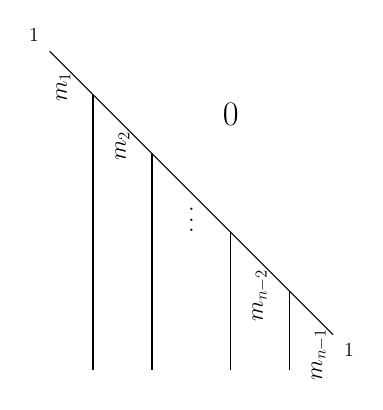
\begin{tikzpicture}[
                baseline=(current bounding box.center),
                scale=0.5,
                transform shape,
                every node/.style={inner sep=1pt}
            ]
            \node at (0, 0) {\Large $1$};
            \node at (8, -8) {\Large $1$};

            \draw (0.4, -0.4) -- (7.6, -7.6);
            \node at (5, -2) {\Huge $0$};

            \foreach \x in {1.5, 3.0, 5.0, 6.5} {
                \draw (\x, -\x) -- (\x, -8.5);
            }

            \node[rotate=90, anchor=east] at (0.75, -0.9) {\LARGE $m_1$};
            \node[rotate=90, anchor=east] at (2.25, -2.4) {\LARGE $m_2$};
            \node[rotate=90, anchor=east] at (4.0, -4.2) {\LARGE $\dots$};
            \node[rotate=90, anchor=east] at (5.75, -5.9) {\LARGE $m_{n-2}$};
            \node[rotate=90, anchor=east] at (7.25, -7.4) {\LARGE $m_{n-1}$};
        \end{tikzpicture}
    \right)
\]

\subsection{Fattorizzazione di Cholesky}

\begin{snippettheorem}{Fattorizzazione di Cholesky}
    \(A = A^\ast\) definita positiva se e solo se
    esiste unica \(V\) triangolare inferiore con \(V_{j,j} > 0\) tale che \(A = VV^\ast\).
\end{snippettheorem}

\begin{snippetproof}{Fattorizzazione di Cholesky}
    \begin{iffproof}
    \item \(A=A^\ast\) definita positiva se e solo se ogni minore principale è definita positiva.
        In particolare, lo sono i minori principali di testa, che quindi sono invertibili ovvero \(A\)
        è fortemente non singolare.
        Esiste un'unica \(L\) triangolare inferiore con \(L_{j,j} = 1\) ed un'unica
        \(U\) triangolare superiore tale che \(A = LU\).
        Scriviamo
        \begin{align*}
            A &= LU = L \operatorname{diag}_j (U_{j,j}) \tilde U
        \end{align*}
        dove \(\tilde U\) è \(U\) ma con tutti gli elementi sopra la diagonale divisi per \(U_{j,j}\),
        così possiede \(1\) sulla diagonale.
        Allora \(A = A^\ast = \tilde U^\ast \operatorname{diag}_j (U_{j,j}) L^\ast\).
        Ma quindi \(\tilde U^\ast\) è una triangolare inferiore con \(1\) sulla diagonale.
        L'altro termine prodotto è una triangolare superiore.
        La forte non singolarità implica pure l'unicità della fattorizzazione, quindi deve essere
        \[
            L = \tilde U^\ast, \quad U = \operatorname{diag}_j (\tilde U_{j,j}) L^\ast
        \]
        Abbiamo quindi trovato che
        \begin{align*}
            A &= L \cdot \operatorname{diag}_j (U_{j,j}) L^\ast
        \end{align*}
        Gli \(U_{j,j}\) sono reali perché coniugano, ma sono anche in \(\realnumbers^{>0}\)
        in quanto \(A\) è definita positiva.
        Siccome \(L\) ha uno sulla diagonale ed è triangolare inferiore è invertibile.
        Scegliamo quindi \(v^{(j)} = (L^\ast)^{-1}e_j\). Con questa scelta,
        \[
            0 < v_{(j)}^\ast A v_{(j)} = e_j^T \operatorname{diag}_j(U_{j,j})e_j
        \]
        Abbiamo quindi che \[
            A = L \operatorname{diag}_j(U_{j,j}) L^\ast
            = \underbrace{L \operatorname{diag}_j(\sqrt{U_{j,j}})}_{V}
            \underbrace{\operatorname{diag}_j(\sqrt{U_{j,j}})L^\ast}_{V^\ast}
        \]
    \item Sappiamo che \(A = VV^\ast\) con \(V_{j,j} > 0\) e \(V\) triangolare inferiore,
        quindi è sicuramente invertibile.
        Abbiamo che \(A^\ast = (VV^\ast)^\ast = V^{\ast\ast}V^\ast = VV^\ast = A\),
        quindi è Hermitiana.
        Inoltre, \(\forall x \neq 0\) abbiamo
        \begin{DispWithArrows*}
            x^\ast A x &= x^\ast V V^\ast x \Arrow{\(y = V^\ast x\)} \\
            &= y^\ast y = ||y||_2^2 > 0
        \end{DispWithArrows*}
        siccome \(V\) è invertibile \(y \neq 0\).
    \end{iffproof}
\end{snippetproof}

\pagebreak

L'algoritmo è anche un criterio per testare la definita positività di una matrice.
Data una Hermitiana, proviamo l'algoritmo: se funziona è definita positiva, altrimenti non lo è.
L'algoritmo è un algoritmo compatto.
Prendiamo \(A \in \matrices_{n}(\complexnumbers)\)
come input ed imponiamo che \(VV^* = A\), e si risolve l'equazione
rispetto alle incognite, cioè alle entrate di \(V\).
Abbiamo quindi una matrice

\[
    \left(
        \begin{array}{c|c|c|c}
            \mathbf{V_{1,1}} &        &        & 0 \\
            & \mathbf{V_{2,2}} &       &   \\
            V_1     &      & \ddots &   \\
            &  V_2       &        & \mathbf{V_{n,n}}
        \end{array}
    \right)
    \left(
        \begin{array}{cccc}
            \mathbf{V_{1,1}} &   &    V_1^*     &   \\
            \hline
            & \mathbf{V_{2,2}} &  &  V_2^*  \\
            \hline
            &         & \ddots &   \\
            \hline
            0       &         &        & \mathbf{V_{n,n}}
        \end{array}
    \right)
    =
    \left(
        \begin{array}{c|c|c|c}
            \mathbf{A_{1,1}} &        &        & \ast \\
            & \mathbf{A_{2,2}} &       &      \\
            A_1     &      & \ddots &     \\
            &   A_2      &        & \mathbf{A_{n,n}}
        \end{array}
    \right)
\]
dove \(A_i,V_i\) sono le sotto-colonne relativamente all'elemento della diagonale
delle rispettive matrici. L'idea è di isolare iterativamente ogni \(A_{i,i}\)
e risolvere per \(V_{i,i}\), e le sottocolonne rispettive. \\
\textbf{Passo 1:} per la prima colonna, imponiamo \(V_{1,1}^2 = A_{1,1}\)
e quindi \(V_{1,1} = \sqrt{A_{1,1}}\).
Otteniamo quindi \(V_{1,1} \cdot V_1\)
da cui \(V_1 = \frac{A_1}{V_{1,1}}\)
Abbiamo eseguito \(n-1\) operazioni (1 operazione per ogni elemento). \\
\textbf{Passo 2:} per la colonna due, abbiamo
\[
    |V_{2,1}|^2 + V_{2,2}^2 \rightarrow V_{2,2} = \sqrt{A_{2,2} - |V_{2,1}|^2}
\]
Abbiamo eseguito \(3\) operazioni.
Denotiamo con \(\tilde V_i\) la coda di \(V_i\).
Abbiamo ora la colonna di dimensione \(n-2\) data da
\(\overline V_{2,1} \tilde V_{1} + V_{2,2} V_2 = A_2\).
Precedentemente non abbiamo usato il coniugato su \(V_{1,1}\)
in quanto sapevamo che fosse positivo. Otteniamo quindi che
\[
    V_2 = \frac{A_2 - \overline V_{2,1} \tilde V_{1}}{V_{2,2}}
\]
Abbiamo ora eseguito \(3(n-2)\) operazioni (3 operazioni per ogni elemento). \\
\textbf{Passo 3:} continuando otteniamo
\[
    |V_{3,1}|^2 + |V_{3,2}|^2 + V_{3,3}^2 = A_{3,3}
\]
e qua abbiamo \(5(n-3)\) operazioni (5 operazioni per ogni elemento).
In generale la dimensione dei vettori scende mentre il numero di operazioni sale. \\
In totale abbiamo (senza contare quello diagonale che è di ordine inferiore) \[
    \sum_{k=1}^{n-1} (2k-1)(n-k)
    = (2n+1)\sum_{k=1}^{n-1} k - 2\sum_{k=1}^{n-1} k^2 - n(n-1)
    = \frac{1}{3}n^3 + \mathcal O(n^2)
\]
che è esattamente la metà della complessità dell'algoritmo di Gauss.
Tuttavia, l'algoritmo di Gauss applicato ad una matrice Hermitiana ha la stessa complessità.

\pagebreak

\begin{snippettheorem}{}
    Sia \(A \in \matrices_n(\complexnumbers)\) una matrice definita positiva ed Hermitiana.
    Allora, \(A\) è fortemente non singolare.
\end{snippettheorem}

\begin{snippetproof}{}
    Consideriamo \(\mathcal I, \mathcal J \subseteq \{1, \cdots, n\}\),
    ossia \(\mathcal I = \{i_1, \cdots, i_p\}\)
    e \(\mathcal J = \{j_1, \cdots, j_q\}\)
    con
    \begin{align*}
        1 &\leq i_1 < i_2 \cdots < i_p < n \\
        1 &\leq j_1 < j_2 \cdots < j_q < n
    \end{align*}
    Denotiamo con \(A_{\mathcal I, \mathcal J} \in \complexnumbers^{p \times q}\)
    un generico minore di dimensione \(p \times q\) che contiene gli elementi di indici \(\mathcal I\) incrociati con \(\mathcal J\).
    Abbiamo allora l'elemento
    \[
        \left(A_{\mathcal I, \mathcal J}\right)_{s,t}
        = A_{i_s, j_t}
    \]
    Un tale minore è quadrato se e solo se \(p=q\).
    Un tale minore è un minore principale se e solo se \(\mathcal I = \mathcal J\).
    Un tale minore è un minore principale di testa se \(\mathcal I = \mathcal J = \{1, \cdots, p\}\). \\
    Osserviamo che, da Schur, il fatto che \(A\) sia definita positiva ed Hermitiana
    implica che tutti gli autovalori siano reali positivi.
    Dunque, \(\det A > 0\).
    L'idea della dimostrazione è quella di utilizzare questa affermazione su ogni minore principale di testa.
    Abbiamo che ogni minore principale di \(A\) (in particolare pure quelli di testa)
    sono a loro volta definiti positivi. Sia \(A_{\mathcal I} \triangleq A_{\mathcal I, \mathcal I}\).
    Osserviamo che \[
        \left(A_{\mathcal I}^*\right)_{s,t}
        = \overline{A}_{i_t, i_s}
        = A_{i_s, i_t}
        =\left(A_{\mathcal I}\right)_{s,t}
    \]
    Per studiare la definita positività, studiamo se \(x^* A_{\mathcal I} x > 0\)
    per \(x \in \complexnumbers^p\) con \(x \neq 0\).
    Definiamo \(y_x \in \complexnumbers^n\) come vettore esteso, cioè
    \begin{align*}
        (y_x)_l =
        \begin{cases}
            0 & l \notin \{1, \cdots, p\} \\
            x_s & l = i_s \\
        \end{cases}
    \end{align*}
    Con questa notazione troviamo
    \begin{align*}
        x^* A_{\mathcal I} x
        = y_x^* A y_x
    \end{align*}
    Abbiamo che \(x \neq 0 \implies y_x \neq 0\).
    Abbiamo quindi la definita positività sui minori principali, e riutilizzando l'argomento precedente
    ciascun minore principale di testa è invertibile. Quindi, la matrice è fortemente non singolare.
\end{snippetproof}

Dal procedimento precedente si evince che sulle definite positive e Hermitiane
si può applicare sia l'eliminazione gaussiana senza pivot, sia
l'algoritmo per la fattorizzazione di Cholesky.

Durante l'algoritmo di Gauss su una matrice Hermitiana,
normalizzando i pivot dal primo all'ultimo,
il blocco non ancora normalizzato è una sottomatrice che rimane Hermitiana (induzione).
Se \(A\) è la nuova matrice ad un passo e \(B\) è quella vecchia, allora \(\overline A_{k,j} = B_{j,k}\),
quindi il costo dell'algoritmo si dimostra ed è quindi equivalente a Cholesky.
L'algoritmo di Gauss è ottimale fra gli algoritmi con scambi di righe e colonne, ma può essere battuto usando
algoritmi ricorsivi.

\pagebreak

\begin{snippettheorem}{Lo spettro commuta con la moltiplicazione di matrici}
    Siano \(A,B \in \matrices_n(\complexnumbers)\).
    Allora, \(\sigma(AB) = \sigma(BA)\).
\end{snippettheorem}

\begin{snippetproof}{Lo spettro commuta con la moltiplicazione di matrici}
    Se \(A\) è invertibile, \(BA = A^{-1}ABA\) ovvero sono simili e hanno
    il medesimo polinomio caratteristico
    \[
        p_{AB}(\lambda) = p_{BA}(\lambda)
    \]
    In particolare, gli autovalori coincidono.
    Analogamente con \(B\). Ci manca il caso dove sia \(A\) che \(B\)
    sono singolari. In tal caso,
    sia \(A = QTQ^*\) con \(Q\) unitaria e \(T\) triangolare superiore.
    Sia \(\varepsilon > 0\) e sia
    \[
        A_\varepsilon \triangleq QT_\varepsilon Q^*
    \]
    che è invertibile, dove
    \((T_{\varepsilon})_{j,j} = \varepsilon\) se \((T_{\varepsilon})_{j,j} = 0\)
    e il resto uguale a \(T\).
    Cioè sulla diagonale ci sono gli autovalori, e sostituiamo gli zeri con degli \(\varepsilon\),
    visto che è triangolare inferiore rimane invertibile perché il prodotto è non nullo.
    Riconducendoci al caso invertibile, vale
    \[
        p_{A_\varepsilon B}(\lambda) = p_{BA_\varepsilon}(\lambda)
    \]
    Se \(A_\varepsilon \to A\) per \(\varepsilon \to 0\), allora per un argomento di continuità
    pure i polinomi caratteristici tendono a quelli di \(AB\) e \(BA\)
    \[
        p_{AB}(\lambda) = p_{BA}(\lambda)
    \]
\end{snippetproof}

\begin{snippettheorem}{}
    Siano \(A \in \complexnumbers^{n \times m}\) e \(B \in \complexnumbers^{m \times n}\).
    Allora, \(\sigma(AB) = \sigma(BA)\) a meno di \(n-m\) (se \(n-m > 0\))
    o \(m-n\) (se \(m-n > 0\)) zeri laddove servono.
\end{snippettheorem}

\begin{snippetproof}{}
    Supponiamo senza perdita di generalità che \(m \geq n\).
    Vogliamo ricondurci al caso quadrato, e quindi consideriamo
    \[
        A_{\text{ext}}=
        \left(
            \begin{array}{c|c}
                & 0 \\
                A & \vdots \\
                & 0
            \end{array}
        \right)
        \in \matrices_{n}(\complexnumbers),
        \qquad
        B_{\text{ext}}=
        \left(
            \begin{array}{ccc}
                & B & \\ \hline
                \multicolumn{3}{c}{0 \cdots 0}
            \end{array}
        \right)
        \in \matrices_{n}(\complexnumbers)
    \]
    con un numero appropriato di zeri per completarla.
    Visto che le matrici sono quadrate,
    \[
        \sigma(A_{\text{ext}}B_{\text{ext}})
        = \sigma(B_{\text{ext}}A_{\text{ext}})
    \]
    Ma notiamo che nel prodotto \(A_{\text{ext}}B_{\text{ext}}\) riga per colonna, ritroviamo \(AB\),
    e quindi lo spettro è precisamente quello di \(AB\).
    Invece, il prodotto inverso \(B_{\text{ext}}A_{\text{ext}}\)
    notiamo che otteniamo un blocco quadrato \[
        B_{\text{ext}}A_{\text{ext}} =
        \left(
            \begin{array}{c|c}
                BA & 0 \\
                \hline
                0 & 0
            \end{array}
        \right)
        = \operatorname{diag}(BA, 0_{n-m})
    \]
    quindi lo spettro coincide.
\end{snippetproof}

Questo teorema vale nel caso particolare (già visto)
\(m=1\). Infatti, \(\sigma(xy^*) = \{y^*x, 0, 0, \cdots, 0\}\)
con \(x,y \in \complexnumbers^n\), cioè il caso della diade, che ha rango uno.

\subsection{Matrici semi-elementari e aggiornamenti a basso rango}

Abbiamo visto che dato \(I + xy^*\)
con \(x,y \in \complexnumbers^n\)
possiamo caratterizzarne lo spettro e la condizione di invertibilità:
\(g^*x \neq -1\) e in tal caso
\[
    \left(I + xy^*\right)^{-1} = I - \frac{xy^*}{1 + y^*x}
\]
Quindi in generale sappiamo tutto delle diadi \(xy^*\).
Tuttavia, nell'esercizio avevamo una matrice di rango 2.
In generale, al posto di sommare una matrice di rango \(1\),
sommiamo una matrice di rango \(k\), vale lo stesso ragionamento.

Consideriamo quindi \(I + R\)
con \(\operatorname{rank} R = r\) (generalmente molto più piccolo di \(n\)).
Scrivendo \(R\) come righe, sappiamo che esistono \(r\)
vettori \(v_1, \cdots, v_r\) linearmente indipendenti tali che
\begin{align*}
    R &=
    \left[
        \begin{array}{c}
            \text{riga}_1 \\ \hline
            \text{riga}_2 \\ \hline
            \vdots \\ \hline
            \text{riga}_n
        \end{array}
    \right]
    &= \left[
        \begin{array}{c}
            \sum_{s=1}^r \alpha_{1,s} v_s \\ \hline
            \sum_{s=1}^r \alpha_{2,s} v_s \\ \hline
            \vdots \\ \hline
            \sum_{s=1}^r \alpha_{n,s} v_s
        \end{array}
    \right]
    = \underbrace{
        \begin{pmatrix}
            \alpha_{1,1} & \alpha_{1,2} & \cdots & \alpha_{1,r} \\
            \alpha_{2,1} & \alpha_{2,2} & \cdots & \alpha_{2,r} \\
            \vdots & \vdots & \ddots & \vdots \\
            \alpha_{n,1} & \alpha_{n,2} & \cdots & \alpha_{n,r}
        \end{pmatrix}
    }_{r}
    \left[
        \begin{array}{ccc}
            & v_1 & \\ \hline
            & v_2 & \\ \hline
            \vdots \\ \hline
            & v_n &
        \end{array}
    \right]
\end{align*}
Quindi la nuova condizione non è più che \(g^*x \neq -1\),
ma che \(XY^*\) non abbia l'autovalore \(-1\), in quanto se avesse un tale autovalore,
la matrice originale avrebbe autovalore \(1 - 1 = 0\).

Abbiamo quindi che lo spettro è dato da \(1\)
con molteplicità \(n - r\)
e gli altri autovalori sono
\[
    1 + \sigma(YX^*)
\]
con molteplicità \(1\).
Quindi se \(YX^*\) non ha l'autovalore \(-1\), \(I + R\)
è invertibile. In tal caso,
\[
    (I + XY^*)^{-1}
    = I - X \left(I_r + Y^*X\right)^{-1} Y^*
\]
che è una generalizzazione della forma scalare.

\pagebreak

Verifichiamo che sia l'inversa:
\begin{align*}
    \left(I - X \left(I_r + Y^*X\right)^{-1} Y^*\right)
    (I + XY^*)
    &= I + XY^* - X \left(I_r + Y^*X\right)^{-1}Y^*
    - X \left(I_r + Y^*X\right)^{-1} Y^*XY^* \\
    &= I + X\left(
        I - (I_r + Y^*X)^{-1} - (I_r + Y^*X)^{-1}Y^*X
    \right)Y^* \\
    &= I + X \left(I_r + Y^*X\right)^{-1} \left(
        I_r + Y^*X - I_r - Y^*X
    \right)Y^*
    = I
\end{align*}

\begin{snippetproposition}{}
    Sia \(E = I_n + UV^*\) con
    \(U,V \in \complexnumbers^{n \times k}\).
    Allora
    \begin{enumerate}
        \item Gli autovalori di \(E\)
            sono \(1\) con molteplicità algebrica (almeno) \(n-k\)
            e \(1 + \sigma_i(V^*U)\)
            con \(i \in \{1, \cdots, k\}\).
            Nel caso in cui \(\operatorname{rank} U = \operatorname{rank} V = k\)
            allora gli autovalori non nulli sono quelli di \(V^*U\).
        \item Dagli autovalori dati ricaviamo che \(E\) è invertibile se e solo
            se \(-1\) non è un autovalore di \(V^*U\).
        \item Se \(E\) è invertibile allora la sua inversa è
            \[
                E^{-1}
                = I_n - U(I_k + V^*U)^{-1}V^*
            \]
    \end{enumerate}
\end{snippetproposition}

Il costo della rappresentazione dell'inversa
è \[
    k^2(2n-1) + \mathcal O(k^3)
\]

\subsection{Formula di Sherman--Morrison--Woodbury}

La formula di \emph{Sherman-Morrison-Woodbury}
non è altro che la formula dell'inversa appena data ma reinterpretata nel caso di correzione di rango
(al più \(k\)) di una matrice invertibile \(A\).

Sia \(B = A + UV^*\)
con \(\det A \neq 0\)
e ci riconduciamo al caso di matrici semi-elementari scrivendo
\(B = A(I + A^{-1} U V^*)\).
Allora a questo punto, dalla condizione classica sugli autovalori,
ricaviamo che \(B\) è invertibile se e solo se
\(I_k + V^*A^{-1}U\) è invertibile, cioè se e solo se \(-1\) non è un autovalore di \(V^*A^{-1}U\).
Stiamo quindi usando \(A^{-1}U\) come termine.
Quindi la matrice è invertibile se e solo se \(V^* A^{-1} U\)
non possiede l'autovalore \(-1\).
In tal caso, rappresentiamo la matrice come
\[
    B^{-1} = \left(
        I_n - A^{-1} U(I_k + V^* A^{-1} U)^{-1}V^*
    \right)^{-1}A^{-1}
\]

Quindi se siamo bravi a risolvere sistemi con \(A\)
possiamo correggere il sistema per la matrice \(B\).
Se \(\det A = 0\)
ha senso comunque procedere ma rispetto al problema ai quadrati minimi,
che è un senso più debole di risoluzione del sistema associato.
Dato un sistema \(By=c\), come preprocessimo dobbiamo per forza calcolare
\[
    W = A^{-1}U
\]
cioè \(A^{-1}v_1, \cdots, A^{-1} v_{k}\),
che sono \(k\) sistemi lineari in \(A\).
Chiaramente \(A^{-1}\) la calcoliamo solo una volta.
Sostituendo
\[
    B^{-1} c = (I_n - W(I_k + V^* A^{-1} U)^{-1}V^*)A^{-1} c
\]
In termini computazionali abbiamo \(k+1\) risoluzioni con matrice \(A\).
Nel caso volessimo risolvere molteplici sistemi lineari con \(B\)
allora mettiamo pure \(V^* A^{-1}\) nel preprocessing.

Esiste un criterio di vicinanza fra matrici dove due matrici sono vicine se
il rango della differenza diviso la dimensione è piccolo,
oltre che la distanza in norma. Esiste una topologia che tiene conto sia della distanza in
norma che secondo questo criterio.

\begin{snippettheorem}{Teorema di Lusin (Extra)}
    Data \(f \in L^\infty([0,1])\) e \(\varepsilon >0\),
    cioè limitata quasi ovunque. Allora
    \(\exists f_\varepsilon\) continua in \([0,1]\) ed un dominio che
    copre quasi tutto \(\Omega_\varepsilon \subseteq [0,1]\)
    tale che \(\mu(\Omega_\varepsilon) \geq 1-\varepsilon\) tale che
    \[
        \restr{f}{\Omega_\varepsilon} = f_\varepsilon
    \]
\end{snippettheorem}

Questo è un corrispettivo di considerare
\[
    \operatorname{rank}(B_n - B) = d_n = o(n)
\]
dove \(n\) è la dimensione.
Quindi relativamente a tutto lo spazio il rango è piccolo.

\pagebreak

\section{Norme vettoriali e matriciali}

\subsection{Norma infinito e norma indotta}

Abbiamo la norma infinito
\[
    ||x||_\infty = \max_j |x_j|
\]
per \(x \in \complexnumbers^n\).
Allora abbiamo
\begin{DispWithArrows*}
    ||A||_\infty &= \sup_{x\neq 0} \frac{||Ax||_\infty}{||x||_\infty} \\
    &= \sup_{x \neq 0} \left|\left|A \frac{x}{||x||_\infty}\right|\right| \\
    &= \sup_{||x||_\infty = 1} ||Ax||_\infty \Arrow{Compattezza} \\
    &= \max_{||x||_\infty = 1} ||Ax||_\infty \\
    &= \max_{||x||_\infty = 1} \max_j \left|
    \sum_{k=1}^n A_{j,k} x_k
    \right| \\
    &\leq \max_j \sum_{k=1}^n |A_{j,k}| \\
    &= \left|\left|
    \begin{pmatrix}
        ||\text{row}_1||_\infty \\
        ||\text{row}_2||_\infty \\
        \vdots \\

        ||\text{row}_n||_\infty \\
    \end{pmatrix}
    \right|\right| \Arrow{per qualche \(p\)} \\
    &= ||\text{row}_p||_1 = \sum_{i=1}^n \left|A_{p,i}x_i\right| \Arrow{\(A_{p,i} = |A_{p,i}|e^{i\varphi_i}\)} \\
    &
    \begin{cases}
        x_1 = e^{-i\varphi_1} \\
        x_2 = e^{-i\varphi_2} \\
        \cdots \\
        x_n = e^{-i\varphi_n}
    \end{cases}
\end{DispWithArrows*}

\begin{snippetexercise}{}
    Con la stessa dimostrazione, considerare
    \[
        A(f)(x) = \int_X K(x,t)f(t)\,\text{d}t,
        \quad A \colon \mathcal C[D] \fromto \mathcal C[D]
    \]
    calcolare
    \[
        \sup_{||f||_\infty \leq 1} ||A(f)(x)||_\infty = \sup_{x\in D} \int_D |K(x,t)|\,\text{d}t
    \]
\end{snippetexercise}

Come costruire norme nuove in generale?
Sia \(||\cdot||_\ast\) su \(\complexnumbers^n\) e \(S \in \matrices_n(\complexnumbers)\) invertibile.
Allora possiamo definire
\(||\cdot||_{\ast, S} \triangleq ||S \cdot||_\ast\), e quindi per ogni vettore
\(y \in \complexnumbers^n\) definire
\[
    ||y||_{\ast, S} = ||Sy||_\ast \geq 0
\]
Abbiamo
\begin{enumerate}
    \item \(||y||_{\ast, S} = 0\) se e solo se, per definizione \(||Sy||_{\ast} = 0\)
        se e solo se \(Sy = 0\), in quanto pure \(||\cdot||_{\ast}\) è una norma, se e solo se \(y=0\).
    \item Sia \(\alpha \in \complexnumbers, y \in \complexnumbers^n\).
        Abbiamo che \[
            ||\alpha y||_{\ast, S} = ||S(\alpha y)||_{\ast} = |\alpha| \cdot ||Sy||_{\ast} = |\alpha| \cdot ||y||_{\ast, S}
        \]
    \item Siano \(x,y \in \complexnumbers^n\). Abbiamo che
        \[
            ||x+y||_{\ast, S} = ||S(x+y)||_\ast = ||Sx + Sy||_\ast \leq ||Sx||_\ast + ||Sy||_\ast = ||x||_{\ast, S} + ||y||_{\ast, S}
        \]
\end{enumerate}
L'invertibilità di \(S\) serve solo per la prima.

Un altro modo di costruire una norma è quello di fare una combinazione lineare non negativa di altre norme.
\[
    \sum a_j ||\cdot||_{\ast, x_j},
    \quad ||\cdot||_{x_1}, \cdots, ||\cdot||_{x_k} \text{ norme su } \complexnumbers^n
\]
In particolare le combinazioni convesse sono ancora norme.
Questo potrebbe essere usato nella creazione di un esame.

Dato \(V \in \matrices_n(\complexnumbers)\) studiamo \(||V||_{\ast, S}\). Abbiamo
\begin{DispWithArrows*}
    ||V||_{\ast, S} &= \sup_{x \neq 0} \frac{||Vx||_{\ast, S}}{||x||_{\ast, S}} = \sup_{x \neq 0} \frac{||SVx||_{\ast}}{||Sx||_{\ast}} \Arrow{\(y= Sx\)} \\
    &= \sup_{y \neq 0} \frac{||SVS^{-1}y||_\ast}{
        ||y||_\ast
    } = ||SVS^{-1}||_\ast
\end{DispWithArrows*}
La sostituzione è valida in quanto \(S\) è invertibile e quindi mappa \(\complexnumbers^n\)
in \(\complexnumbers^n\) e ovviamente \(0\) in \(0\).

\begin{snippettheorem}{}
    Sia \(A \in \matrices_n(\complexnumbers)\).
    Allora,
    \[
        \rho(A) = \inf_{\substack{||\cdot||\, \text{norma} \\ \text{matriciale indotta}}} ||A||
    \]
\end{snippettheorem}

\begin{snippetproof}{}
    Sappiamo che per ogni norma matriciale indotta \(||\cdot||\) \[
        \rho(A) \leq ||A||
    \]
    Sia \(\varepsilon > 0\) arbitrariamente piccolo.
    Cerchiamo una norma matriciale indotta particolare
    \(||\cdot||_{\ast, \varepsilon}\) tale che
    \[
        ||A||_{\ast, \varepsilon} \leq \rho(A) + \varepsilon
    \]
    Se troviamo tale norma allora vale la tesi.
    La norma dipende sia da \(A\) che da \(\varepsilon\).
    Scriviamo \(A = TJT^{-1}\) con la scomposizione di Jordan.
    Consideriamo una norma \(||\cdot||_{\ast, S}\) con \(S\) invertibile. Sappiamo che
    \[
        ||V||_{\ast, S} = ||SVS^{-1}||_\ast
    \]
    Dobbiamo scegliere \(S\) appropriatamente.
    Scegliamo \(S = F T^{-1}\) per qualche \(F\) (e \(T\) dipende dalla \(A\)).
    Visto che \(T\) dipende solo da \(A\), \(F\) (che deve essere invertibile per il teorema di Binet)
    dovrà presumibilmente dipendere da \(\varepsilon\).
    Da questa scomposizione otteniamo la semplificazione
    \begin{align*}
        ||A||_{\ast, S} &= ||FT^{-1}(TJT^{-1})TF^{-1}||_{\ast}
        = ||FJF^{-1}||_\ast
    \end{align*}
    Ricordiamo che \(J\) è bidiagonale superiore (autovalori sulla diagonale, valori \(\pm 1\) sulla sopradiagonale).
    Scegliamo \(||\cdot||_\ast = ||\cdot||_\infty\).
    Dobbiamo scegliere \(F\) in maniera tale che il prodotto faccia uscire precisamente gli \(\varepsilon\).
    Cerchiamo una \(F\) diagonale in maniera tale che la moltiplicazione scali le righe e le colonne.
    Vogliamo che gli elementi \((j,j+1)\)
    \[
        (FJF^{-1})_{j,j+1} =
        \frac{F_{j,j}\ast}{F_{j+1, j+1}} = \varepsilon \cdot \ast
    \]
    Allora scegliamo
    \[
        F^{-1} = \operatorname{diag}(1, \varepsilon, \varepsilon^2, \cdots, \varepsilon^{n-1})
    \]
    cioè
    \[
        F = \operatorname{diag}(1, \varepsilon^{-1}, \varepsilon^{-2}, \cdots, \varepsilon^{1-n})
    \]
    Se i valori sulla diagonale superiore sono \(0\), allora tutto funziona, il problema era quando sono \(1\).
    Abbiamo quindi in conclusione
    \begin{align*}
        ||A||_{\infty, FT^{-1}} &=
        \left|\left|
        \begin{pmatrix}
            \lambda_1 & \ast & & & \\
            & \lambda_2 & \ast & & \\
            & & \ddots & \ddots &  \\
            & & & \lambda_n & \ast
        \end{pmatrix}
        \right|\right|_\infty \leq \max_j |\lambda_j + \ast \varepsilon| \leq \rho(A) + \varepsilon
    \end{align*}
\end{snippetproof}

Abbiamo quindi un invariante algebrico nel teorema sugli spazi di Banach per questo motivo.

\subsection{Norme indotte \(1\), \(2\) e infinito}

Abbiamo visto la norma matriciale indotta dalla norma infinito. Studiamo ora i casi
con norma \(1\) e \(2\).
Partiamo dal caso di \(||\cdot||_1\).
Ci chiediamo qual è la corrispondente norma matriciale indotta
Abbiamo
\begin{DispWithArrows*}
    ||A||_1 &= \max_{||x||_1 = 1} ||Ax||_1
    = \max_{||x||_1 = 1} \left|\left|
    \sum_{j=1}^n x_j \text{col}_j(A)
    \right|\right|_1 \Arrow{Disuguaglianza \\ triangolare} \\
    &= \max_{||x||_1 = 1}
    \sum_{j=1}^n |x_j| \cdot || \text{col}_j(A)||_1 \\
    &= \left(\underbrace{\max_{||x||_1 = 1} \sum_{j=1}^n |x_j|}_1\right)
    \max_j ||\text{col}_j A||_1 \\
    &= \max_j ||\text{col}_j(A)||_1
\end{DispWithArrows*}
Per completare e dimostrare l'uguaglianza
bisogna esibire un particolare vettore per il quale abbiamo l'uguaglianza.
Un tale \(\hat x\) ha \(||\hat x||_1\)
e \[
    ||A\hat x||_1 = \max_j ||\text{col}_j(A)||_1 = ||\text{col}_p(A)||_1
\]
e scegliamo \(\hat x = e_p\),
così selezioniamo precisamente la colonna \(p\).
Per le norme infinite guardavamo la righe mentre qua le colonne.

Passiamo ora alla norma \(2\).
Sia \(V\) Hermitiana e definita positiva, quindi ordiamo
\[
    \lambda_1(V) \leq \cdots \leq \lambda_n(V)
\]
e vale
\[
    \lambda_1(V) = \min_{x \neq 0} \frac{x^* V x}{x^* x},
    \quad
    \lambda_n(V) = \max_{x \neq 0} \frac{x^* V x}{x^* x}
\]
Possiamo scrivere minimo e massimo al posto di infinimum e supremum in quanto
possiamo restringerci ad un compatto. Quello che importa è l'angolazione, non andare verso infinito.
Per la norma indotta abbiamo
\begin{align*}
    ||A||_2 &= \max_{x \neq 0} \frac{||Ax||_2}{||x||_2}
    = \max_{x \neq 0} \frac{\sqrt{x^* A^* A x}}{\sqrt{x^* x}} \\
    &= \sqrt{
        \max_{x \neq 0} \frac{x^* V x}{x^* x}
    } \\
    &= \sqrt{
        \rho(A^* A)
    }
\end{align*}
Essendo definita positiva, raggio spettrale e autovalore massimo sono la stessa cosa
(per il modulo).

\begin{snippetproposition}{}
    Se \(A\) è normale,
    allora \(A = QDQ^*\) con \(D\) diagonale complessa.
    Ma allora
    \[
        A^* A = Q \operatorname{diag}(|\lambda_i|^2)Q^*
    \]
    in quanto
    \[
        \lambda_{\text{max}}(A^*A) = \max_j |\lambda_j(A)|^2 = \rho(A)
    \]
    e la norma indotta è
    \[
        ||A||_2 = \rho(A)
    \]
\end{snippetproposition}

Quindi questo vale non solo per le Hermitiane.

\pagebreak

\section{Decomposizione ai valori singolari}

Notiamo che la parola decomposizione è distinta da una fattorizzazione
e non è nemmeno una forma normale.

\begin{snippettheorem}{Decomposizione ai valori singolari}
    Sia \(A \in \complexnumbers^{n \times m}\).
    Allora, \(\exists U \in \matrices_n(\complexnumbers), V \in \matrices_m(\complexnumbers)\)
    unitarie ed \(\exists ! \Sigma \in \realnumbers_{\geq 0}^{n \times m}\)
    con \(\Sigma\) tale che \(\Sigma_{j,k} = 0\) se \(j \neq k\)
    e tale che \[
        A = U \Sigma U, \quad
        \Sigma_{j,j} = b_j, j \in \{1, \cdots, \min\{n,m\}\}
    \]
    dove \(\sigma_j\) sono i \emph{valori singoari}. In particolare,
    \[
        \sigma_1 = ||A||_2
        \geq \sigma_2 \geq \cdots \geq \sigma_p > 0
        = \sigma_{p+1} = \cdots = \sigma_{\min\{n,m\}}
    \]
    quindi \(p\) è il rango di \(A\).
\end{snippettheorem}

Nel processing delle immagini viene utilizzata questa decomposizione in quanto
la gran parte dell'informazione
è contenuta nel rango basso.

\begin{snippetproof}{Decomposizione ai valori singolari}
    Distinguiamo due casi.
    \begin{itemize}
        \item \(n \geq m:\)
            procediamo per induzione su \(m\). Il caso base è
            \((n, 1)\). Abbiamo quindi \(A\) vettore con elementi \(a\).
            Consideriamo la matrice di Hausholder \[
                Ha =
                \begin{pmatrix}
                    \alpha \\ 0 \\ \vdots \\ 0
                \end{pmatrix},
                \quad H = I - \frac{2vv^*}{||v||_2}
            \]
            Ma quindi \(\alpha = |\alpha| e^{i\theta}\),
            e sostituendo
            \[
                Ha =
                \begin{pmatrix}
                    |\alpha| \\ 0 \\ \vdots \\ 0
                \end{pmatrix}\left[
                    e^{i\theta}
                \right],
                \quad a = H
                \begin{pmatrix}
                    |\alpha| \\ 0 \\ \vdots \\ 0
                \end{pmatrix}
                \left[e^{i\theta}\right]
            \]
            Notando che le matrici unitarie mantengono la norma due,
            per completare osserviamo che
            \[
                |a| = ||A||_2
            \]
            Sia ora \(A \in \complexnumbers^{n \times m}\)
            e \(m \geq 2\).
            Notiamo che
            \[
                ||A||_2 = \max_{||x||_2 = 1} ||Ax||
            \]
            che oviamo essere il nostro \(\sigma_1\).
            Essendo un massimo, ci deve essere un vettore che lo realizza.
            Sia \(\hat x\) tale che \(||\hat x|| = 1\) e
            \(y = A\hat x\) con \(||y||_2 = ||A||_2\).
            Definiamo quindi
            \[
                \hat V =
                \left[
                    \begin{array}{c|c|c|c}
                        & & & \\
                        \hat x & s_2 & \cdots & s_m \\
                        & & &
                    \end{array}
                \right] \in \matrices_m(\complexnumbers)
            \]
            Costruiamo un'altra unitaria
            \[
                \hat U = \left[
                    \begin{array}{ccc}
                        \frac{1}{||A||}y^* & & \\ \hline
                        & t_2^* &  \\ \hline
                        & \vdots & \\ \hline
                        & t_n^* &
                    \end{array}
                \right] \in \matrices_n(\complexnumbers)
            \]
            Studiamo quindi
            \begin{align*}
                \hat U A \hat V
                &= \hat U \left[
                    \begin{array}{c|c|c|c}
                        & & & \\
                        y & \hat s_2 & \cdots & \hat s_n \\
                        & & &
                    \end{array}
                \right]
            \end{align*}
            Ma eseguendo il prodotto troviamo
            \[
                \frac{1}{||A||}y^*y = \frac{||y||^2}{||A||^2} = ||A||
            \]
            quindi il primo elemento in testa è \(||A||\)
            \[
                \hat U A \hat V = \left[
                    \begin{array}{c|ccc}
                        ||A|| &  & c^* & \\ \hline
                        0 & & & \\
                        \vdots & & \hat A & \\
                        0 & & &
                    \end{array}
                \right]
            \]
            Tuttavia non possiamo ancora applicare l'ipotesi induttiva.
            Ricordiamo che \(||Pv||_2 = ||v||_2\) sempre per ogni \(P\) unitaria.
            Ma allora,
            \begin{DispWithArrows*}
                ||\hat U A \hat V||_2 &= \max_{||x||=1} ||\hat U A \hat Vx||_2 \Arrow{\(y = \hat Vx\)} \\
                &= \max_{||y||_2 = 1} ||\hat H Ay||_2
                = \max_{||y||_2 = 1} ||Ay||_2 = ||A||
            \end{DispWithArrows*}
            Vogliamo mostrare che \(c^*\) deve essere nullo.
            Per mostrarlo scegliamo un vettore che lo mostra, denotando \(B = \hat U A \hat V\)
            \begin{DispWithArrows*}
                ||B||_2 &\geq
                \left|\left|
                B
                \begin{pmatrix}
                    ||A||_2 \\ c
                \end{pmatrix}
                \right|\right|_2
                \cdot \frac{1}{\left|\left|
                    \begin{pmatrix}
                        ||A||_2 \\ c
                    \end{pmatrix}
                \right|\right|} \\
                &= \frac{1}{\sqrt{
                        ||A||_2^2 + ||c||_2^2
                }} \left|\left|
                \begin{pmatrix}
                    ||A||_2^2 + ||c||_2^2 \\
                    \hat A c
                \end{pmatrix}
                \right|\right|_2 \Arrow{Minoriamo con \\ \(\hat A c = 0\)} \\
                &\geq \left|\left|
                \begin{pmatrix}
                    ||A||_2^2 + ||c||_2^2 \\
                    0 \\ \vdots \\ 0
                \end{pmatrix}
                \right|\right|_2 \\
                &= \frac{
                    ||A|_2^2 + ||c||_2^2
                }{
                    \sqrt{
                        ||A||_2^2 + ||c||_2^2
                    }
                } \\
                &= \sqrt{||A||_2^2 + ||c||^2} \geq ||A||_2
            \end{DispWithArrows*}
            Ma se \(c\) avesse anche solo una componente non-nulla, allora avremmo
            il segno maggiore stretto. Ma quindi, deve essere per forza \(c=0\).
            Siccome \(c=0\), possiamo applicare l'ipotesi induttiva e segue il teorema
            Allora scriviamo \[
                \hat A = \tilde U \tilde \Sigma \tilde V
            \]
            con \(\tilde \Sigma_{1,1} \geq \tilde \Sigma_{2,2} \geq \cdots\).
            Troviamo quindi
            \begin{align*}
                \hat U A \hat V &= \left[
                    \begin{array}{c|ccc}
                        ||A||_2 & 0 & \cdots & 0 \\ \hline
                        0 & & & \\
                        \vdots & & \hat A & \\
                        0 & & &
                    \end{array}
                \right]
                = \left[
                    \begin{array}{c|ccc}
                        ||A||_2 & 0 & \cdots & 0 \\ \hline
                        0 & & & \\
                        \vdots & & \tilde U \tilde \Sigma \tilde V & \\
                        0 & & &
                    \end{array}
                \right] \\
                &= \left[
                    \begin{array}{c|ccc}
                        1 & 0 & \cdots & 0 \\ \hline
                        0 & & & \\
                        \vdots & & \tilde U& \\
                        0 & & &
                    \end{array}
                \right]
                \left[
                    \begin{array}{c|ccc}
                        ||A||_2 & 0 & \cdots & 0 \\ \hline
                        0 & & & \\
                        \vdots & & \tilde \Sigma & \\
                        0 & & &
                    \end{array}
                \right]
                \left[
                    \begin{array}{c|ccc}
                        1 & 0 & \cdots & 0 \\ \hline
                        0 & & & \\
                        \vdots & & \tilde V & \\
                        0 & & &
                    \end{array}
                \right] \\
                A &= \underbrace{\hat U^*
                    \left[
                        \begin{array}{c|ccc}
                            1 & 0 & \cdots & 0 \\ \hline
                            0 & & & \\
                            \vdots & & \tilde U& \\
                            0 & & &
                        \end{array}
                \right]}_{U}
                \underbrace{\left[
                        \begin{array}{c|ccc}
                            ||A||_2 & 0 & \cdots & 0 \\ \hline
                            0 & & & \\
                            \vdots & & \tilde \Sigma & \\
                            0 & & &
                        \end{array}
                \right]}_{\Sigma}
                \underbrace{\left[
                        \begin{array}{c|ccc}
                            1 & 0 & \cdots & 0 \\ \hline
                            0 & & & \\
                            \vdots & & \tilde V & \\
                            0 & & &
                        \end{array}
                    \right]
                \hat V^*}_{V}
            \end{align*}
            che hanno la forma giusta e soddisfano tutte le proprietà per ipotesi induttiva.
            Inoltre, quando ricaviamo la norma di \(||A||_2\) nel caso base,
            la norma è unica. Per induzione questa rimane unica.
        \item \(n < m:\) Sia \(B = A^*\). Adesso possiamo utilizzare il primo caso
            \[
                B = A^* = U_B \Sigma_B V_B,
                \quad \Sigma_B
                = \operatorname{diag}(\sigma_1(B), \sigma_2(B), \cdots, \sigma_p(B), 0, \cdots, 0)
            \]
            Con le proprietà che
            \[
                \sigma_1(B) = ||B||_2
                \geq \sigma_2(B) \geq \cdots \geq \sigma_p(B) > 0
                = \sigma_{p+1}(B) = \cdots = \sigma_m(B)
            \]
            Riapplicando la trasposta coniugata otteniamo
            \[
                A = B^* = V_B^* \Sigma_B^T U_B^*
            \]
            dove \(V_B^*\) è unitaria in \(\matrices_n(\complexnumbers)\)
            e \(U_B^*\) è unitaria in \(\matrices_m(\complexnumbers)\).
            Scegliendo quindi \(U = V_B^*, \Sigma = \Sigma_B^T\) e \(V = U_B^*\),
            troviamo la tesi se mostriamo anche le proprietà aggiuntive.
            Sappiamo che \(p = \operatorname{rank}(B) = \operatorname{rank}(A)\)
            e che \[
                \sigma_1(B) = ||B||_2 = \sqrt{\rho(B^*B)} =
                \sqrt{\rho(A A^*)} = \sqrt{\rho(A^*A)}
                = ||A||_2 = \sigma_1(A)
            \]
            usando la commutazione degli autovalori (gli zeri aggiuntivi nello spettro non ci interessano).
    \end{itemize}
\end{snippetproof}

Nel caso normale, i moduli degli autovalori sono i valori singolari
dopo averli ordinati.

\pagebreak

\section{Approssimazione polinomiale e operatori positivi}

\subsection{Operatori positivi e polinomi di Bernstein}

Consideriamo lo spazio \(\mathcal C([0,1])\)
di funzioni continue a valori reali su \([0,1]\).
Vogliamo esibire una successione \(P_n(x)\)
di polinomi tale che \[
    ||f-P_n||_{\infty, [0,1]} \to 0
\]
per \(n \to +\infty\).

\begin{snippetdefinition}{Operatore lineare positivo}
    Sia
    \[
        \phi \colon (\mathcal A, \leq_{\mathcal A}) \fromto (\mathcal B, \leq_{\mathcal B})
    \]
    Diciamo che \(\phi\) è \emph{lineare positivo} (LPO) se
    \(\mathcal A, \mathcal B\)
    spazi vettoriali con ordinamenti parziali tale che:
    \begin{enumerate}
        \item \[
                \phi(\alpha f  + \beta g) = \alpha \phi(f) + \beta\phi(g)
            \]
            per ogni \(f,g \in \mathcal A\)
            e per ogni \(\alpha,\beta \in \mathbb K\) campo.
        \item Se \(f \geq_{\mathcal A} 0_{\mathcal A}\) allora \[
                \phi(f) \geq_{\mathcal B} 0_{\mathcal B}
            \]
    \end{enumerate}
\end{snippetdefinition}

\begin{snippetdefinition}{Polinomi di Bernstein}
    Consideriamo \(\mathcal C([0,1])\) e \(f \in \mathcal C([0,1])\).
    Un \emph{polinomio di Bernstein} è definito come
    \[
        B_n(f)(x) = \sum_{k=0}^n f\left(\frac kn\right) \binom{n}{k} x^k (1-x)^{n-k}
    \]
    con \(B_n \colon \mathcal C([0,1]) \fromto \mathcal C([0,1])\).
    Equipaggiamo inoltre l'ordinamento \(f \geq g\) se e solo se
    \(f(x) \geq g(x)\) per ogni \(x \in [0,1]\).
\end{snippetdefinition}

Se fosse stato uno spazio \(L^p\) al posto di un per ogni avremmo un quasi ovunque.
L'oggetto \(B_n\) è un polinomio di grado al più \(n\), in quanto combinazione lineari di tali.

\begin{snippetproposition}{}
    \(B_n\) è un endooperatore lineare positivo in \(\mathcal C([0,1])\) per ogni \(n\).
\end{snippetproposition}

\begin{snippetproof}{}
    Siano \(\alpha, \beta \in \realnumbers\) e \(f,g \in \mathcal C([0,1])\).
    Abbiamo
    \begin{align*}
        B_n(\alpha f + \beta g)(x) &= \sum_{n=0}^n \left(\alpha f + \beta g\right)\left(\frac{k}{n}\right)
        \binom{k}{n} x^k(1-x)^{n-k} \\
        &= \sum_{n=0}^n \left(
            \alpha f\left(\frac{n}{k}\right) + \beta g\left(\frac{n}{k}\right)
        \right) x^k(1-x)^{n-k} \\
        &= \alpha \sum_{k=0}^n f\left(\frac kn\right) \binom{n}{k} x^k (1-x)^{n-k}
        + \beta \sum_{k=0}^n g\left(\frac kn\right) \binom{n}{k} x^k (1-x)^{n-k} \\
        &= \alpha B_n(f) + \beta B_n(g)
    \end{align*}
    quindi è lineare. Per la positività vediamo,
    se \(f \geq 0\) allora \(f\left(\sfrac kn\right) \geq 0\) e quindi dalla definizione
    una serie di termini positivi su \([0,1]\).
\end{snippetproof}

\begin{snippetproposition}{}
    Un operatore lineare positivo \(\phi \colon \mathcal C([0,1]) \to \mathcal C([0,1])\)
    è monotono e isotono.
\end{snippetproposition}

\begin{snippetproof}{}
    \begin{enumerate}
        \item per la monotonia notiamo che \(f-g \geq 0\), allora
            \(\phi(f-g) \geq 0\), ma quindi per linearità \(\phi(f) - \phi(g) \geq 0\)
            cioè \(\phi(f) \leq \phi(g)\).
        \item per l'isotonia notiamo che \(-|f| \leq f \leq |f|\).
            Per la monotonia abbiamo che \(-\phi(|f|) \leq \phi(f) \leq \phi(|f|)\)
            da cui troviamo che \(|\phi(f)| \leq phi(|f|)\).
    \end{enumerate}
\end{snippetproof}

Gli integrali di funzioni positive sono operatori lineari positivi.

\begin{snippettheorem}{Teorema di Korovkin in una dimensione}
    Sia \(\{\phi_n\}\) una successione di endooperatori lineari positivi su
    \(\mathcal C(K)\), con \(K\) compatto di \(\realnumbers\).
    Supponiamo che \[
        ||\phi_n(y^j)(x) - x^j||_{\infty, K} \to 0
    \]
    per \(n \to +\infty\) con \(j=0,1,2\), allora
    \(\forall f \in \mathcal C(K)\), \[
        \left|\left|
        \phi_n(f(y)) - f(x)
        \right|\right|_{\infty, K} \to 0
    \]
    per \(n \to +\infty\).
\end{snippettheorem}

\begin{snippetproof}{}
    Scriviamo \[
        \phi_n(y^j)(x) = x^j + \varepsilon_n^{(j)}(x),
        \quad \left|\left|
        \varepsilon_n^{(j)}(x)
        \right|\right|_{\infty, K} \to 0
    \]
    per \(n \to \infty\).
    Fissiamo \(f \in \mathcal C(K)\) e fissiamo \(\varepsilon > 0\).
    Dobbiamo trovare \(n_\varepsilon\) tale che \(\forall n \geq n_\varepsilon\)
    \[
        \Delta_n(f,x) \triangleq |\phi_n(f(y))(x) - f(x)| \leq \varepsilon, \quad \forall x \in K
    \]
    Quel \(\forall x \in K\) ci dà la convergenza uniforme.
    Scriviamo ora
    \begin{DispWithArrows*}
        \Delta_n(f,x) &= |\phi_n(f(y))(x) - (\phi_n(1)(x) - \varepsilon_n^{(0)}(x))f(x)| \\
        &= |\phi_n(f(y))(x) - f(x) \cdot \phi_n(1)(x) + \varepsilon_n^{(0)}(x)f(x)| \Arrow{Disuguaglianza \\ triangolare} \\
        &\leq |\phi_n(f(y))(x) - f(x) \phi_n(1)(x)| + ||\varepsilon_n^{(0)}||_{\infty, K}
        \cdot ||f||_{\infty, K} \\
        &\leq |\phi_n(f(y))(x) - f(x)\phi_n(1)(x)| + \sfrac{\varepsilon}{3}, \quad \forall n \geq n_\varepsilon \\
        &= |\phi_n(f(y) - f(x))(x)| + \sfrac{\varepsilon}{3} \Arrow{positività} \\
        &\leq \phi_n(|f(y) - f(x)|)(x) + \sfrac{\varepsilon}{3}
    \end{DispWithArrows*}
    Visto che siamo su un compatto, la continuità implica la continuità uniforme, quindi
    \(\forall \tilde \varepsilon > 0\) esiste \(\tilde \delta > 0\) tale che
    se \(|x-y| < \tilde \delta\) allora \(|f(y) - f(x)| < \tilde \varepsilon\)
    per tutte le \(x,y \in K\).
    Siccome questa ultima condizione vale solo quando \(|y-x| < \tilde \delta\), possiamo estenderla scrivendo
    \[
        |f(y) - f(x)| \leq \tilde \varepsilon +
        2||f||_{\infty, K} \chi_{\{y \suchthat \tilde \delta \leq |y-x|\}}(y)
    \]
    Infatti, quando \(|y-x| < \tilde \delta\) usiamo la continuità uniforme, mentre nell'altro caso
    maggioriamo \(|f(y)-f(x)|\) con \(|f(y)| + |f(x)|\), e a loro volta maggioriamo ognuno di questi con
    \(||f||_{\infty, K}\).
    Per \(y\) tale che \(|y-x| \geq \tilde \delta\), vale che
    \(\sfrac{|y-x|}{\tilde \delta} \geq 1\), ma questo è equivalente a dire che
    \(\sfrac{(y-x)^2}{\tilde \delta^2} \geq 1\).
    Quindi possiamo aggiornare la maggiorazione a
    \begin{align*}
        |f(y) - f(x)| &\leq \tilde \varepsilon + 2||f||_{\infty, K}
        \frac{(y-x)^2}{\tilde \delta^2}
    \end{align*}
    Sostituendo questa troviamo che per monotonia
    \begin{DispWithArrows*}
        \Delta_n(f,x) &\leq \phi_n\left(
            \frac{y^2 - 2xy + x^2}{\tilde \delta^2}
            \cdot 2||f||_{\infty, K} + \tilde\varepsilon
        \right)(x) + \frac{\varepsilon}{3} \\
        &= \tilde\varepsilon\phi_n(1)(x) + 2\frac{||f||_{\infty, K}}{\tilde\delta^2}
        \left[
            \phi_n(y^2)(x) - 2x\phi_n(y)(x) + x^2\phi_n(1)(x)
        \right] + \frac{\varepsilon}{3} \\
        &= \tilde\varepsilon(1 + \varepsilon_n^{(0)}(x)) + 2\frac{||f||_{\infty, K}}{\tilde \delta^2}
        \left[
            x^2 + \varepsilon_n^{(2)}(x) - 2x\left(x + \varepsilon_n^{(1)}(x)\right)
            + x^2\left(1 + \varepsilon_n^{(0)}(x)\right)
        \right] + \frac{\varepsilon}{3} \Arrow{Scegliendo \\ \(\tilde\varepsilon = \sfrac{\varepsilon}{6}\)} \\
        &\leq \frac{2}{3}\varepsilon + 2\frac{||f||_{\infty, K}}{\tilde \delta^2}
        \left|
        \varepsilon_n^{(2)}(x) - 2x\varepsilon_n^{(1)}(x) + x^2 \varepsilon_n^{(0)}(x)
        \right|
    \end{DispWithArrows*}
    dove abbiamo anche scelto \(n_\varepsilon\) abbastanza grande da avere
    \(||\varepsilon_n^{(0)}||_{\infty, K} \leq 1\).
    Poiché \(K\) è compatto, poniamo \[
        \hat M = \sup_{x \in K}|x| < +\infty.
    \]
    Otteniamo quindi la successione numerica che va a zero
    \begin{align*}
        Q_n &\triangleq \frac{2||f||_{\infty, K}}{\tilde \delta^2} \left(
            ||\varepsilon_n^{(2)}||_{\infty, K} + 2 \hat M ||\varepsilon_n^{(1)}||_{\infty, K}
            + \hat M^2 ||\varepsilon_n^{(0)}||_{\infty, K}
        \right) < \frac{\varepsilon}{3}
    \end{align*}
    per \(n \geq n_\varepsilon\).
    Quindi, per ogni \(x \in K\), abbiamo \[
        \Delta_n(f,x) \leq \frac{2}{3}\varepsilon + Q_n < \varepsilon,
    \]
    e dunque
    \[
        \left|\left|
        \phi_n(f(y)) - f(x)
        \right|\right|_{\infty, K} \to 0.
    \]
\end{snippetproof}

Il teorema può essere esteso, sotto ipotesi opportune, anche alla convergenza in \(L^p\).

Vediamo il test di Korovkin sugli operatori di Bernstein \(B_n(\cdot)\) su \([0,1]\). Abbiamo
\begin{enumerate}
    \item Vediamo se \(B_n(1)(x)\) converge a \(1\). Abbiamo
        \[
            \sum_{k=0}^n \binom{n}{k}x^k(1-x)^{n-k} = ((1 - x) + x)^n = 1
        \]
        e quindi \(\varepsilon_n^{(0)} = 0\).
    \item Vediamo se \(B_n(y)(x)\) converge a \(x\). Abbiamo
        \begin{align*}
            B_n(y)(x) &= \sum_{k=0}^n \binom{n}{k} \frac{k}{n} x^k(1-x)^{n-k} \\
            &= \sum_{k=1}^n \binom{n}{k} \frac{k}{n} x^k(1-x)^{n-k} \\
            &= x\sum_{k=1}^n \binom{n-1}{k-1} x^{k-1}(1-x)^{n-k} \\
            &= x \cdot \sum_{q = 0}^{n-1} \binom{n-1}{q} x^q (1-x)^{n-1-q} \\
            &= x
        \end{align*}
        quindi \(\varepsilon_n^{(1)} = 0\).
    \item Vediamo se \(B_n(y^2)(x)\) converge a \(x^2\). Per definizione,
        \[
            B_n(f)(x)
            =
            \sum_{k=0}^{n}
            \binom{n}{k}
            f\left(\frac{k}{n}\right)
            x^k(1-x)^{n-k}.
        \]
        Dunque, per \(n\geq 2\),
        \begin{align*}
            B_n(y^2)(x)
            &=
            \sum_{k=0}^{n}
            \binom{n}{k}
            \left(\frac{k}{n}\right)^2
            x^k(1-x)^{n-k} \\
            &=
            \sum_{k=1}^{n}
            \binom{n}{k}
            \left(\frac{k}{n}\right)^2
            x^k(1-x)^{n-k} \\
            &=
            \frac{x}{n}
            \sum_{k=1}^{n}
            k
            \binom{n}{k}
            \frac{k}{n}
            x^{k-1}(1-x)^{n-k}.
        \end{align*}
        Usando l'identità
        \[
            k\binom{n}{k}
            =
            n\binom{n-1}{k-1},
        \]
        otteniamo
        \begin{align*}
            B_n(y^2)(x)
            &=
            x
            \sum_{k=1}^{n}
            \binom{n-1}{k-1}
            \frac{k}{n}
            x^{k-1}(1-x)^{n-k}.
        \end{align*}
        Scriviamo
        \[
            \frac{k}{n}
            =
            \frac{1}{n}
            +
            \frac{n-1}{n}\frac{k-1}{n-1}.
        \]
        Allora
        \begin{align*}
            B_n(y^2)(x)
            &=
            x
            \sum_{k=1}^{n}
            \binom{n-1}{k-1}
            \left(
                \frac{1}{n}
                +
                \frac{n-1}{n}\frac{k-1}{n-1}
            \right)
            x^{k-1}(1-x)^{n-k} \\
            &=
            \frac{x}{n}
            \sum_{k=1}^{n}
            \binom{n-1}{k-1}
            x^{k-1}(1-x)^{n-k} \\
            &\quad
            +
            \frac{x(n-1)}{n}
            \sum_{k=1}^{n}
            \binom{n-1}{k-1}
            \frac{k-1}{n-1}
            x^{k-1}(1-x)^{n-k}.
        \end{align*}
        Facendo il cambio di variabile \(j=k-1\), si ha
        \[
            \sum_{k=1}^{n}
            \binom{n-1}{k-1}
            x^{k-1}(1-x)^{n-k}
            =
            B_{n-1}(1)(x)
            =
            1,
        \]
        mentre
        \[
            \sum_{k=1}^{n}
            \binom{n-1}{k-1}
            \frac{k-1}{n-1}
            x^{k-1}(1-x)^{n-k}
            =
            B_{n-1}(y)(x)
            =
            x.
        \]
        Quindi
        \begin{align*}
            B_n(y^2)(x)
            &=
            \frac{x}{n}
            +
            \frac{x(n-1)}{n}x \\
            &=
            \frac{x}{n}
            +
            \frac{n-1}{n}x^2 \\
            &=
            x^2+\frac{x(1-x)}{n}.
        \end{align*}

        Pertanto, se poniamo
        \[
            \varepsilon_n^{(2)}(x)
            =
            B_n(y^2)(x)-x^2,
        \]
        allora
        \[
            \varepsilon_n^{(2)}(x)
            =
            \frac{x(1-x)}{n}.
        \]
        Poiché
        \[
            0\leq x(1-x)\leq \frac{1}{4}
            \qquad
            \forall x\in[0,1],
        \]
        si ottiene
        \[
            \left\|\varepsilon_n^{(2)}\right\|_{\infty,[0,1]}
            \leq
            \frac{1}{4n}
            \xrightarrow[n\to\infty]{}
            0.
        \]
\end{enumerate}

\begin{snippettheorem}{Teorema di Weierstrass in \(\realnumbers\)}
    Sia \(K\subseteq \realnumbers\) compatto. Per ogni \(f\in C(K)\) esiste una successione di polinomi \(\{P_n\}\) tale che
    \[
        \left\|f-P_n\right\|_{\infty,K}
        \xrightarrow[n\to\infty]{}
        0.
    \]
\end{snippettheorem}

\begin{snippetproof}{}
    Procediamo per passi.

    \medskip

    \noindent
    \textbf{Passo 1: \(K=[0,1]\).}

    Consideriamo gli operatori di Bernstein
    \[
        B_n : C([0,1])\longrightarrow C([0,1]).
    \]
    Per costruzione \(B_n(f)\) è un polinomio di grado al più \(n\). Inoltre \(B_n\) è lineare positivo.

    Abbiamo verificato che
    \[
        B_n(1)=1,
        \qquad
        B_n(X)=X,
        \qquad
        \left\|B_n(X^2)-X^2\right\|_{\infty,[0,1]}\to 0.
    \]
    Quindi \(B_n\) soddisfa il test di Korovkin su \([0,1]\). Per il teorema di Korovkin segue che
    \[
        \left\|B_n(f)-f\right\|_{\infty,[0,1]}
        \xrightarrow[n\to\infty]{}
        0
        \qquad
        \forall f\in C([0,1]).
    \]

    \medskip

    \noindent
    \textbf{Passo 2: \(K=[a,b]\), con \(a<b\).}

    Sia \(f\in C([a,b])\). Definiamo
    \[
        g(t)
        =
        f(a+(b-a)t),
        \qquad t\in[0,1].
    \]
    Allora \(g\in C([0,1])\). Per il passo precedente,
    \[
        \left\|g-B_n(g)\right\|_{\infty,[0,1]}
        \xrightarrow[n\to\infty]{}
        0.
    \]
    Per \(x\in[a,b]\) poniamo
    \[
        t=\frac{x-a}{b-a}.
    \]
    Allora \(t\in[0,1]\) e
    \[
        f(x)=g\left(\frac{x-a}{b-a}\right).
    \]
    Definiamo quindi
    \[
        P_n(x)
        =
        B_n(g)\left(\frac{x-a}{b-a}\right).
    \]
    Essendo composizione di un polinomio con un'affinità, \(P_n\) è un polinomio in \(x\). Inoltre
    \begin{align*}
        \left\|f-P_n\right\|_{\infty,[a,b]}
        &=
        \max_{x\in[a,b]}
        \left|
        f(x)
        -
        B_n(g)\left(\frac{x-a}{b-a}\right)
        \right| \\
        &=
        \max_{t\in[0,1]}
        \left|
        g(t)-B_n(g)(t)
        \right| \\
        &=
        \left\|g-B_n(g)\right\|_{\infty,[0,1]}
        \xrightarrow[n\to\infty]{}
        0.
    \end{align*}

    \medskip

    \noindent
    \textbf{Passo 3: \(K\subseteq\realnumbers\) compatto generico.}

    Scegliamo un intervallo \([a,b]\) tale che
    \[
        K\subseteq(a,b).
    \]
    Per il teorema di estensione di Tietze, per ogni \(f\in C(K)\) esiste \(\widetilde f\in C([a,b])\) tale che
    \[
        \widetilde f_{\mid K}=f.
    \]
    Eventualmente si può scegliere l'estensione in modo che
    \[
        \widetilde f(a)=\widetilde f(b)=0.
    \]

    Per il passo precedente esiste una successione di polinomi \(\{P_n\}\) tale che
    \[
        \left\|\widetilde f-P_n\right\|_{\infty,[a,b]}
        \xrightarrow[n\to\infty]{}
        0.
    \]
    Restringendo a \(K\), otteniamo
    \[
        \left\|f-P_n\right\|_{\infty,K}
        \leq
        \left\|\widetilde f-P_n\right\|_{\infty,[a,b]}
        \xrightarrow[n\to\infty]{}
        0.
    \]
    Questo conclude la dimostrazione.
\end{snippetproof}

\begin{snippetproposition}{Osservazione sul test di Korovkin in dimensione \(1\)}
    Sia \(K=[a,b]\) e sia
    \[
        \Phi:C(K)\longrightarrow C(K)
    \]
    un operatore lineare positivo. Se \(\Phi\) riproduce esattamente le funzioni test
    \[
        1,\qquad X,\qquad X^2,
    \]
    cioè
    \[
        \Phi(1)=1,
        \qquad
        \Phi(X)=X,
        \qquad
        \Phi(X^2)=X^2,
    \]
    allora \(\Phi(f)=f\) per ogni \(f\in C^2(K)\).

    In particolare, per un operatore non banale non ci si aspetta che gli errori del test di Korovkin siano esattamente nulli; è sufficiente che tendano a zero uniformemente.
\end{snippetproposition}

\begin{snippetproof}{}
    Fissiamo \(f\in C^2(K)\) e \(x\in K\). Scriviamo \(Y(t)=t\), per distinguere la variabile della funzione dal punto \(x\) in cui si valuta l'operatore.

    Per il teorema di Taylor, per ogni \(y\in K\) esiste un punto \(\xi_{x,y}\) compreso tra \(x\) e \(y\) tale che
    \[
        f(y)
        =
        f(x)
        +
        f'(x)(y-x)
        +
        \frac{f''(\xi_{x,y})}{2}(y-x)^2.
    \]
    Quindi
    \[
        f(y)-f(x)
        =
        f'(x)(y-x)
        +
        \frac{f''(\xi_{x,y})}{2}(y-x)^2.
    \]
    Applicando \(\Phi\) e usando linearità e positività,
    \begin{align*}
        \left|
        \Phi(f)(x)-f(x)
        \right|
        &=
        \left|
        \Phi(f(Y)-f(x))(x)
        \right| \\
        &\leq
        \left|
        f'(x)\Phi(Y-x)(x)
        \right|
        +
        \frac{1}{2}\left\|f''\right\|_{\infty,K}
        \Phi((Y-x)^2)(x).
    \end{align*}
    Ora
    \[
        \Phi(Y-x)(x)
        =
        \Phi(Y)(x)-x\Phi(1)(x)
        =
        x-x
        =
        0,
    \]
    e
    \begin{align*}
        \Phi((Y-x)^2)(x)
        &=
        \Phi(Y^2-2xY+x^2)(x) \\
        &=
        \Phi(Y^2)(x)-2x\Phi(Y)(x)+x^2\Phi(1)(x) \\
        &=
        x^2-2x^2+x^2 \\
        &=
        0.
    \end{align*}
    Pertanto
    \[
        \left|
        \Phi(f)(x)-f(x)
        \right|
        =0
        \qquad
        \forall x\in K,
    \]
    da cui \(\Phi(f)=f\).
\end{snippetproof}

\begin{snippettheorem}{Teorema di Korovkin in \(\realnumbers^d\)}
    Sia \(K\subseteq\realnumbers^d\) compatto e siano
    \[
        \Phi_n:C(K)\longrightarrow C(K)
    \]
    operatori lineari positivi.

    Supponiamo che
    \[
        \left\|\Phi_n(g)-g\right\|_{\infty,K}
        \xrightarrow[n\to\infty]{}
        0
    \]
    per ogni
    \[
        g\in T,
        \qquad
        T=
        \left\{
            1,
            X_1,\dots,X_d,
            X_1^2+\cdots+X_d^2
        \right\}
    \]
    Allora, per ogni \(f\in C(K)\),
    \[
        \left\|\Phi_n(f)-f\right\|_{\infty,K}
        \xrightarrow[n\to\infty]{}
        0.
    \]
\end{snippettheorem}

\begin{snippetproof}{}
    Indichiamo con
    \[
        \rho(X)=X_1^2+\cdots+X_d^2=\left\|X\right\|^2.
    \]
    L'ipotesi sul test di Korovkin equivale a dire che, per ogni \(g\in T\),
    \[
        \Phi_n(g)(x)
        =
        g(x)+\varepsilon_n^{(g)}(x),
        \qquad
        \left\|\varepsilon_n^{(g)}\right\|_{\infty,K}
        \xrightarrow[n\to\infty]{}
        0
    \]
    Fissiamo \(f\in C(K)\) e \(\varepsilon>0\). Poiché \(K\) è compatto, \(f\) è uniformemente continua. Quindi esiste \(\delta>0\) tale che
    \[
        \left\|y-x\right\|<\delta
        \implies
        |f(y)-f(x)|<\frac{\varepsilon}{3}
        \qquad
        \forall x,y\in K
    \]
    Inoltre, se \(\left\|y-x\right\|\geq\delta\), allora
    \[
        |f(y)-f(x)|
        \leq
        2\left\|f\right\|_{\infty,K}
        \leq
        \frac{2\left\|f\right\|_{\infty,K}}{\delta^2}
        \left\|y-x\right\|^2.
    \]
    Combinando le due stime, otteniamo per ogni \(x,y\in K\):
    \[
        |f(y)-f(x)|
        \leq
        \frac{\varepsilon}{3}
        +
        \frac{2\left\|f\right\|_{\infty,K}}{\delta^2}
        \left\|y-x\right\|^2.
    \]

    Fissiamo ora \(x\in K\). Scrivendo \(Y=(Y_1,\dots,Y_d)\) per la variabile della funzione su cui agisce \(\Phi_n\), abbiamo
    \begin{align*}
        \Phi_n(f)(x)-f(x)
        &=
        \Phi_n(f(Y)-f(x))(x)
        +
        f(x)\left(\Phi_n(1)(x)-1\right).
    \end{align*}
    Pertanto
    \begin{align*}
        \left|\Phi_n(f)(x)-f(x)\right|
        &\leq
        \Phi_n(|f(Y)-f(x)|)(x)
        +
        \left\|f\right\|_{\infty,K}
        \left|\varepsilon_n^{(1)}(x)\right| \\
        &\leq
        \frac{\varepsilon}{3}\Phi_n(1)(x)
        +
        \frac{2\left\|f\right\|_{\infty,K}}{\delta^2}
        \Phi_n(\left\|Y-x\right\|^2)(x)
        +
        \left\|f\right\|_{\infty,K}
        \left|\varepsilon_n^{(1)}(x)\right|.
    \end{align*}

    Studiamo il termine quadratico. Poiché
    \[
        \left\|Y-x\right\|^2
        =
        \left\|Y\right\|^2
        -
        2\sum_{i=1}^{d}x_iY_i
        +
        \left\|x\right\|^2,
    \]
    si ha
    \begin{align*}
        \Phi_n(\left\|Y-x\right\|^2)(x)
        &=
        \Phi_n(\rho)(x)
        -
        2\sum_{i=1}^{d}x_i\Phi_n(Y_i)(x)
        +
        \left\|x\right\|^2\Phi_n(1)(x) \\
        &=
        \left\|x\right\|^2+\varepsilon_n^{(\rho)}(x)
        -
        2\sum_{i=1}^{d}x_i
        \left(x_i+\varepsilon_n^{(X_i)}(x)\right) \\
        &\quad
        +
        \left\|x\right\|^2
        \left(1+\varepsilon_n^{(1)}(x)\right) \\
        &=
        \varepsilon_n^{(\rho)}(x)
        -
        2\sum_{i=1}^{d}x_i\varepsilon_n^{(X_i)}(x)
        +
        \left\|x\right\|^2\varepsilon_n^{(1)}(x).
    \end{align*}
    Poiché \(K\) è compatto, esiste \(M>0\) tale che
    \[
        \left\|x\right\|\leq M
        \qquad
        \forall x\in K.
    \]
    Dunque
    \[
        \left\|
        \Phi_n(\left\|Y-\cdot\right\|^2)(\cdot)
        \right\|_{\infty,K}
        \xrightarrow[n\to\infty]{}
        0.
    \]

    Inoltre
    \[
        \Phi_n(1)(x)
        =
        1+\varepsilon_n^{(1)}(x),
    \]
    quindi \(\Phi_n(1)\to 1\) uniformemente. Scegliendo \(n\) sufficientemente grande, tutti i termini d'errore precedenti sono minori di quanto serve affinché
    \[
        \left|\Phi_n(f)(x)-f(x)\right|<\varepsilon
        \qquad
        \forall x\in K.
    \]
    Ne segue
    \[
        \left\|\Phi_n(f)-f\right\|_{\infty,K}
        \xrightarrow[n\to\infty]{}
        0.
    \]
\end{snippetproof}

Vogliamo ora dimostrare una versione multidimensionale del teorema di Weierstrass.

\begin{snippettheorem}{Teorema di Weierstrass in \(\realnumbers^d\)}
    Sia \(K\subseteq\realnumbers^d\) compatto. Per ogni \(f\in C(K)\) esiste una famiglia di polinomi \(\{P_{\mathbf n}\}_{\mathbf n}\), con
    \[
        \mathbf n=(n_1,\dots,n_d)\in\naturalnumbers^d,
    \]
    tale che
    \[
        \left\|P_{\mathbf n}-f\right\|_{\infty,K}
        \xrightarrow[\min_i n_i\to\infty]{}
        0.
    \]
    Si può scegliere \(P_{\mathbf n}\) di grado al più \(n_i\) nella variabile \(X_i\).
\end{snippettheorem}

Per dimostrare il risultato, cominciamo definendo i polinomi di Bernstein multidimensionali su \([0,1]^d\).

Siano
\[
    \mathbf n=(n_1,\dots,n_d),
    \qquad
    \mathbf k=(k_1,\dots,k_d),
\]
con
\[
    0\leq k_i\leq n_i
    \qquad
    \forall i=1,\dots,d.
\]
Poniamo
\[
    \binom{\mathbf n}{\mathbf k}
    =
    \prod_{i=1}^{d}
    \binom{n_i}{k_i},
\]
\[
    x^{\mathbf k}
    =
    \prod_{i=1}^{d}
    x_i^{k_i},
    \qquad
    (1-x)^{\mathbf n-\mathbf k}
    =
    \prod_{i=1}^{d}
    (1-x_i)^{n_i-k_i}.
\]
Allora, per \(f\in C([0,1]^d)\), definiamo
\[
    B_{\mathbf n}(f)(x)
    =
    \sum_{k_1=0}^{n_1}
    \cdots
    \sum_{k_d=0}^{n_d}
    f\left(
        \frac{k_1}{n_1},
        \dots,
        \frac{k_d}{n_d}
    \right)
    \prod_{i=1}^{d}
    \binom{n_i}{k_i}
    x_i^{k_i}
    (1-x_i)^{n_i-k_i}.
\]
In notazione multi-indice:
\[
    B_{\mathbf n}(f)(x)
    =
    \sum_{\mathbf k=0}^{\mathbf n}
    \binom{\mathbf n}{\mathbf k}
    f\left(\frac{\mathbf k}{\mathbf n}\right)
    x^{\mathbf k}
    (1-x)^{\mathbf n-\mathbf k},
\]
dove
\[
    \frac{\mathbf k}{\mathbf n}
    =
    \left(
        \frac{k_1}{n_1},
        \dots,
        \frac{k_d}{n_d}
    \right).
\]

\begin{snippetproof}{Dimostrazione del teorema di Weierstrass in \(\realnumbers^d\)}
    Consideriamo prima il caso \(K=[0,1]^d\).

    Gli operatori \(B_{\mathbf n}\) sono lineari positivi. Inoltre,
    \[
        B_{\mathbf n}(1)=1.
    \]
    Per ogni \(i=1,\dots,d\), poiché la variabile \(X_i\) dipende solo dalla \(i\)-esima coordinata,
    \[
        B_{\mathbf n}(X_i)=X_i.
    \]
    Analogamente, usando il calcolo unidimensionale già fatto,
    \[
        B_{\mathbf n}(X_i^2)(x)
        =
        x_i^2+\frac{x_i(1-x_i)}{n_i}.
    \]
    Quindi
    \begin{align*}
        B_{\mathbf n}(X_1^2+\cdots+X_d^2)(x)
        &=
        \sum_{i=1}^{d}
        B_{\mathbf n}(X_i^2)(x) \\
        &=
        \sum_{i=1}^{d}
        x_i^2
        +
        \sum_{i=1}^{d}
        \frac{x_i(1-x_i)}{n_i}.
    \end{align*}
    Perciò
    \[
        \left|
        B_{\mathbf n}(X_1^2+\cdots+X_d^2)(x)
        -
        (X_1^2+\cdots+X_d^2)(x)
        \right|
        =
        \sum_{i=1}^{d}
        \frac{x_i(1-x_i)}{n_i}.
    \]
    Siccome
    \[
        0\leq x_i(1-x_i)\leq\frac14,
    \]
    segue che
    \[
        \left\|
        B_{\mathbf n}(X_1^2+\cdots+X_d^2)
        -
        (X_1^2+\cdots+X_d^2)
        \right\|_{\infty,[0,1]^d}
        \leq
        \frac{d}{4\min_i n_i}
        \xrightarrow[\min_i n_i\to\infty]{}
        0.
    \]
    Dunque \(B_{\mathbf n}\) soddisfa il test di Korovkin multidimensionale. Pertanto
    \[
        \left\|B_{\mathbf n}(f)-f\right\|_{\infty,[0,1]^d}
        \xrightarrow[\min_i n_i\to\infty]{}
        0
        \qquad
        \forall f\in C([0,1]^d).
    \]

    Consideriamo ora un rettangolo
    \[
        Q=
        [a_1,b_1]\times\cdots\times[a_d,b_d].
    \]
    Per \(f\in C(Q)\), definiamo
    \[
        g(t_1,\dots,t_d)
        =
        f\left(
            a_1+(b_1-a_1)t_1,
            \dots,
            a_d+(b_d-a_d)t_d
        \right),
    \]
    con \(t=(t_1,\dots,t_d)\in[0,1]^d\).
    Allora \(g\in C([0,1]^d)\). Definiamo
    \[
        P_{\mathbf n}(x)
        =
        B_{\mathbf n}(g)
        \left(
            \frac{x_1-a_1}{b_1-a_1},
            \dots,
            \frac{x_d-a_d}{b_d-a_d}
        \right).
    \]
    Allora \(P_{\mathbf n}\) è un polinomio in \(x_1,\dots,x_d\), di grado al più \(n_i\) nella variabile \(x_i\), e
    \[
        \left\|P_{\mathbf n}-f\right\|_{\infty,Q}
        =
        \left\|B_{\mathbf n}(g)-g\right\|_{\infty,[0,1]^d}
        \xrightarrow[\min_i n_i\to\infty]{}
        0.
    \]

    Infine, se \(K\subseteq\realnumbers^d\) è compatto generico, scegliamo un rettangolo \(Q\) tale che
    \[
        K\subseteq \operatorname{int}(Q).
    \]
    Per il teorema di estensione di Tietze, ogni \(f\in C(K)\) ammette un'estensione \(\widetilde f\in C(Q)\) con
    \[
        \widetilde f_{\mid K}=f.
    \]
    Per quanto appena dimostrato, esiste una famiglia di polinomi \(\{P_{\mathbf n}\}_{\mathbf n}\) tale che
    \[
        \left\|\widetilde f-P_{\mathbf n}\right\|_{\infty,Q}
        \xrightarrow[\min_i n_i\to\infty]{}
        0.
    \]
    Restringendo a \(K\), si ottiene
    \[
        \left\|f-P_{\mathbf n}\right\|_{\infty,K}
        \leq
        \left\|\widetilde f-P_{\mathbf n}\right\|_{\infty,Q}
        \xrightarrow[\min_i n_i\to\infty]{}
        0.
    \]
\end{snippetproof}

\subsection{Korovkin multidimensionale e polinomi di Bernstein}

L'obiettivo è verificare le ipotesi del teorema di Korovkin per gli operatori di Bernstein su \([0,1]^d\). In questo modo si ottiene una dimostrazione del teorema di Weierstrass in più variabili: ogni funzione continua su un compatto rettangolare può essere approssimata uniformemente da polinomi.

\begin{snippetdefinition}{Operatore di Bernstein in \(d\) variabili}
    Sia \(D=[0,1]^d\) e sia \(\mathbf n=(n_1,\ldots,n_d)\), con \(n_i\in\naturalnumbers\). Per \(f\in C(D)\) definiamo
    \[
        B_{\mathbf n}(f)(x)
        =
        \sum_{k_1=0}^{n_1}\cdots\sum_{k_d=0}^{n_d}
        f\left(\frac{k_1}{n_1},\ldots,\frac{k_d}{n_d}\right)
        \prod_{i=1}^d \binom{n_i}{k_i}x_i^{k_i}(1-x_i)^{n_i-k_i},
    \]
    per ogni \(x=(x_1,\ldots,x_d)\in D\).

    La notazione \(\mathbf n\to\infty\) significa che \(\min_i n_i\to\infty\).
\end{snippetdefinition}

L'operatore \(B_{\mathbf n}\) è un polinomio in \(x_1,\ldots,x_d\), di grado al più \(n_i\) nella variabile \(x_i\). Per applicare Korovkin dobbiamo controllare le funzioni test
\[
    1,\qquad y_1,\ldots,y_d,\qquad \|y\|_2^2=y_1^2+\frac{}{}\cdots+y_d^2.
\]

\begin{snippetproposition}{Linearità e positività}
    Per ogni \(\mathbf n\), l'operatore \(B_{\mathbf n}:C(D)\to C(D)\) è lineare e positivo.
\end{snippetproposition}

\begin{snippetproof}{}
    La linearità segue direttamente dalla definizione. Infatti, per \(\alpha,\beta\in\realnumbers\),
    \begin{align*}
        B_{\mathbf n}(\alpha f+\beta g)(x)
        &=
        \sum_{k_1=0}^{n_1}\cdots\sum_{k_d=0}^{n_d}
        (\alpha f+\beta g)\left(\frac{k_1}{n_1},\ldots,\frac{k_d}{n_d}\right)
        \prod_{i=1}^d \binom{n_i}{k_i}x_i^{k_i}(1-x_i)^{n_i-k_i}\\
        &=
        \alpha B_{\mathbf n}(f)(x)+\beta B_{\mathbf n}(g)(x).
    \end{align*}
    Inoltre, se \(f\geq 0\) su \(D\), allora ogni valore
    \[
        f\left(\frac{k_1}{n_1},\ldots,\frac{k_d}{n_d}\right)
    \]
    è non negativo e tutti i pesi
    \[
        \prod_{i=1}^d \binom{n_i}{k_i}x_i^{k_i}(1-x_i)^{n_i-k_i}
    \]
    sono non negativi su \([0,1]^d\). Quindi \(B_{\mathbf n}(f)(x)\geq 0\) per ogni \(x\in D\).
\end{snippetproof}

\begin{snippetproposition}{Verifica delle funzioni test di Korovkin}
    Per \(\mathbf n\to\infty\) valgono le convergenze uniformi
    \[
        B_{\mathbf n}(1)\to 1,
        \qquad
        B_{\mathbf n}(y_j)\to y_j \quad j=1,
        \ldots,d,
        \qquad
        B_{\mathbf n}(\|y\|_2^2)\to \|y\|_2^2.
    \]
\end{snippetproposition}

\begin{snippetproof}{}
    Per la funzione costante \(1\), usando la formula binomiale in ogni variabile,
    \begin{align*}
        B_{\mathbf n}(1)(x)
        &=
        \sum_{k_1=0}^{n_1}\cdots\sum_{k_d=0}^{n_d}
        \prod_{i=1}^d \binom{n_i}{k_i}x_i^{k_i}(1-x_i)^{n_i-k_i}\\
        &=
        \prod_{i=1}^d \sum_{k_i=0}^{n_i}\binom{n_i}{k_i}x_i^{k_i}(1-x_i)^{n_i-k_i}\\
        &=
        \prod_{i=1}^d (x_i+1-x_i)^{n_i}=1.
    \end{align*}
    Dunque \(B_{\mathbf n}(1)=1\) esattamente.

    Sia ora \(y_j(x)=x_j\). Nella variabile \(j\)-esima compare il momento primo della distribuzione binomiale, mentre nelle altre variabili compare la somma dei pesi, uguale a \(1\):
    \begin{align*}
        B_{\mathbf n}(y_j)(x)
        &=
        \left(\prod_{i\neq j} B_{n_i}(1)(x_i)\right) B_{n_j}(y)(x_j)\\
        &=
        x_j.
    \end{align*}
    Quindi anche in questo caso la convergenza è esatta.

    Infine calcoliamo il momento secondo. In una variabile si ha
    \[
        B_n(y^2)(x)=x^2+\frac{x(1-x)}{n}.
    \]
    Perciò, in \(d\) variabili,
    \begin{align*}
        B_{\mathbf n}(y_j^2)(x)
        &=
        x_j^2+\frac{x_j(1-x_j)}{n_j},\\
        B_{\mathbf n}(\|y\|_2^2)(x)
        &=
        \sum_{j=1}^d B_{\mathbf n}(y_j^2)(x)\\
        &=
        \sum_{j=1}^d x_j^2+
        \sum_{j=1}^d \frac{x_j(1-x_j)}{n_j}\\
        &=
        \|x\|_2^2+
        \sum_{j=1}^d \frac{x_j(1-x_j)}{n_j}.
    \end{align*}
    Poiché \(0\leq x_j(1-x_j)\leq 1/4\), otteniamo
    \[
        \left\|B_{\mathbf n}(\|y\|_2^2)-\|y\|_2^2\right\|_{\infty,D}
        \leq
        \frac14\sum_{j=1}^d \frac1{n_j}
        \xrightarrow[\mathbf n\to\infty]{}0.
    \]
\end{snippetproof}

\begin{snippettheorem}{Teorema di Weierstrass su \([0,1]^d\)}
    Per ogni \(f\in C([0,1]^d)\) si ha
    \[
        \|B_{\mathbf n}(f)-f\|_{\infty,[0,1]^d}
        \xrightarrow[\mathbf n\to\infty]{}0.
    \]
    In particolare, ogni funzione continua su \([0,1]^d\) è limite uniforme di polinomi.
\end{snippettheorem}

\begin{snippetproof}{}
    Gli operatori \(B_{\mathbf n}\) sono lineari e positivi. Inoltre abbiamo appena verificato la convergenza uniforme sulle funzioni test
    \[
        1,\quad y_1,
        \ldots,y_d,
        \quad \|y\|_2^2.
    \]
    Per il teorema di Korovkin in dimensione \(d\), segue che
    \[
        \|B_{\mathbf n}(f)-f\|_{\infty,[0,1]^d}\to 0
    \]
    per ogni \(f\in C([0,1]^d)\). Siccome \(B_{\mathbf n}(f)\) è un polinomio, otteniamo l'approssimazione uniforme tramite polinomi.
\end{snippetproof}

Se l'errore di approssimazione fosse identicamente nullo per ogni funzione continua, allora ogni funzione continua sarebbe un polinomio. Il fatto importante è invece che l'errore tende a zero in norma uniforme: si tratta di approssimazione, non di rappresentazione esatta.

\subsection{Interpolazione polinomiale}

Siano \(x_0,\ldots,x_n\in[a,b]\) punti a due a due distinti e siano \(f_0,\ldots,f_n\in\realnumbers\). Esiste un unico polinomio \(p\in\mathbb{P}_n\) tale che
\[
    p(x_j)=f_j,
    \qquad j=0,\ldots,n.
\]
Se \(f\in C([a,b])\), indicando con \(P_n(f)\) il polinomio interpolante di \(f\) sui nodi scelti, la domanda naturale è:
\[
    P_n(f)\xrightarrow[n\to\infty]{} f
    \quad\text{in } C([a,b])?
\]
In generale la risposta è negativa: l'interpolazione polinomiale non è un metodo universalmente convergente per ogni funzione continua e per ogni scelta dei nodi.

\begin{snippettheorem}{Formula dell'errore di interpolazione}
    Sia \(f\in C^{n+1}([a,b])\) e siano \(x_0,
    \ldots,x_n\in[a,b]\) nodi a due a due distinti. Se \(P_n(f)\) è il polinomio interpolante di \(f\) in tali nodi, allora per ogni \(x\in[a,b]\) esiste \(\xi_x\in(a,b)\) tale che
    \[
        f(x)-P_n(f)(x)
        =
        \frac{f^{(n+1)}(\xi_x)}{(n+1)!}
        \prod_{j=0}^n (x-x_j).
    \]
\end{snippettheorem}

\begin{snippetproof}{}
    Se \(x\) coincide con uno dei nodi, allora entrambi i membri sono nulli. Supponiamo quindi che \(x\notin\{x_0,\ldots,x_n\}\). Poniamo
    \[
        W(t)=\prod_{j=0}^n (t-x_j)
    \]
    e fissiamo \(x\). Consideriamo la funzione ausiliaria
    \[
        \varphi(t)
        =
        f(t)-P_n(f)(t)-
        \frac{f(x)-P_n(f)(x)}{W(x)}W(t).
    \]
    Per costruzione \(\varphi(x)=0\). Inoltre, per ogni nodo \(x_j\), si ha \(f(x_j)-P_n(f)(x_j)=0\) e \(W(x_j)=0\), quindi \(\varphi(x_j)=0\). La funzione \(\varphi\) ha dunque almeno \(n+2\) zeri distinti.

    Applicando ripetutamente il teorema di Rolle, \(\varphi'\) ha almeno \(n+1\) zeri distinti, \(\varphi''\) ne ha almeno \(n\), e così via. Alla fine \(\varphi^{(n+1)}\) ha almeno uno zero \(\xi_x\in(a,b)\). Poiché \(P_n^{(n+1)}=0\) e \(W^{(n+1)}=(n+1)!\), otteniamo
    \[
        0=
        \varphi^{(n+1)}(\xi_x)
        =
        f^{(n+1)}(\xi_x)
        -
        \frac{f(x)-P_n(f)(x)}{W(x)}(n+1)!.
    \]
    Da cui
    \[
        f(x)-P_n(f)(x)
        =
        \frac{f^{(n+1)}(\xi_x)}{(n+1)!}W(x)
        =
        \frac{f^{(n+1)}(\xi_x)}{(n+1)!}
        \prod_{j=0}^n (x-x_j).
    \]
\end{snippetproof}

\begin{snippetexample}{Interpolazione di \(e^x\) su \([0,1]\)}
    Sia \(f(x)=e^x\) e siano \(x_0,
    \ldots,x_n\in[0,1]\) nodi a due a due distinti. Poiché \(f^{(n+1)}(x)=e^x\), si ha
    \[
        \left|f^{(n+1)}(\xi_x)\right|\leq e
        \qquad \text{per ogni } \xi_x\in[0,1].
    \]
    Inoltre \(|x-x_j|\leq 1\) per ogni \(x,x_j\in[0,1]\). Dalla formula dell'errore segue
    \[
        \|e^x-P_n(e^x)\|_{\infty,[0,1]}
        \leq
        \frac{e}{(n+1)!}.
    \]
    Quindi, per questa funzione, l'interpolazione converge uniformemente a \(e^x\), indipendentemente dalla scelta dei nodi in \([0,1]\).
\end{snippetexample}

\begin{snippettheorem}{Non universalità dell'interpolazione: teorema di Faber}
    Per ogni scelta di nodi triangolare
    \[
        x_0^{(n)},\ldots,x_n^{(n)}\in[a,b],
        \qquad n=0,1,2,
    \]
    a due a due distinti per ogni \(n\), esiste una funzione \(f\in C([a,b])\) tale che la successione dei polinomi interpolanti non è uniformemente convergente a \(f\). Più precisamente, si può avere
    \[
        \limsup_{n\to\infty}\|P_n(f)\|_{\infty,[a,b]}=+
        \infty.
    \]
\end{snippettheorem}

Questo risultato mostra che l'interpolazione polinomiale, a differenza dell'approssimazione di Bernstein, non dà automaticamente un procedimento convergente per tutte le funzioni continue.

\section{Metodi per autovalori}

\subsection{Metodo delle potenze}

\begin{snippetdefinition}{Ipotesi spettrale dominante}
    Sia \(A\in M_n(\complexnumbers)\) con autovalori \(\lambda_1,
    \ldots,\lambda_n\) ordinati in modo che
    \[
        |\lambda_1|>|\lambda_2|\geq\cdots\geq |\lambda_n|.
    \]
    L'autovalore \(\lambda_1\) è detto autovalore dominante. Il metodo delle potenze serve ad approssimare \(\lambda_1\) e un suo autovettore.
\end{snippetdefinition}

L'ipotesi \(|\lambda_1|>|\lambda_2|\) è molto comune nelle applicazioni: dice che, iterando la matrice, la componente lungo l'autospazio dominante prevale sulle altre.

\begin{snippetdefinition}{Algoritmo del metodo delle potenze}
    Si scelga \(q^{(0)}\neq 0\) e si ponga
    \[
        x^{(0)}=\frac{q^{(0)}}{\|q^{(0)}\|_\infty}.
    \]
    Per \(k=0,1,2,\ldots\) si ripete:
    \begin{align*}
        q^{(k+1)}&=Ax^{(k)},\\
        p_{k+1}&\in\operatorname{argmax}_{1\leq i\leq n}\left|q_i^{(k+1)}\right|,\\
        \mu^{(k+1)}&=
        \frac{q_{p_{k+1}}^{(k+1)}}{x_{p_{k+1}}^{(k)}},\\
        x^{(k+1)}&=
        \frac{q^{(k+1)}}{\|q^{(k+1)}\|_\infty}.
    \end{align*}
    Ci si ferma quando, fissata una tolleranza \(\varepsilon>0\), vale
    \[
        \frac{|\mu^{(k+1)}-\mu^{(k)}|}{|\mu^{(k+1)}|}\leq \varepsilon,
    \]
    oppure quando si raggiunge un numero massimo di iterazioni.
\end{snippetdefinition}

Se l'algoritmo termina per la prima condizione, allora \(\mu^{(k+1)}\) approssima \(\lambda_1\) e \(x^{(k+1)}\) approssima un autovettore associato, normalizzato in norma \(\infty\).

\begin{snippetproposition}{Analisi nel caso diagonalizzabile}
    Supponiamo che \(A\) sia diagonalizzabile e che \(|\lambda_1|>|\lambda_2|\geq\cdots\geq |\lambda_n|\). Se il vettore iniziale ha componente non nulla lungo l'autovettore dominante, allora il metodo delle potenze converge all'autodirezione dominante.
\end{snippetproposition}

\begin{snippetproof}{}
    Sia \(\{v_1,
    \ldots,v_n\}\) una base di autovettori di \(A\), con
    \[
        Av_j=\lambda_j v_j.
    \]
    Scriviamo
    \[
        x^{(0)}=\alpha_1v_1+
        \alpha_2v_2+
        \cdots+
        \alpha_nv_n,
    \]
    con \(\alpha_1\neq 0\). Allora
    \begin{align*}
        A^k x^{(0)}
        &=
        \alpha_1\lambda_1^k v_1+
        \alpha_2\lambda_2^k v_2+
        \cdots+
        \alpha_n\lambda_n^k v_n\\
        &=
        \lambda_1^k\left(
            \alpha_1v_1+
            \sum_{j=2}^n \alpha_j\left(\frac{\lambda_j}{\lambda_1}\right)^k v_j
        \right).
    \end{align*}
    Poiché
    \[
        \left|\frac{\lambda_j}{\lambda_1}\right|<1
        \qquad j=2,
        \ldots,n,
    \]
    la sommatoria tende a zero. Dunque la direzione di \(A^k x^{(0)}\) tende alla direzione di \(v_1\).

    Più precisamente, per una opportuna costante di normalizzazione \(\gamma_k\),
    \[
        x^{(k)}
        =
        \gamma_k\lambda_1^k\left(
            \alpha_1v_1+O\left(\left|\frac{\lambda_2}{\lambda_1}\right|^k\right)
        \right).
    \]
    Analogamente,
    \[
        q^{(k+1)}=Ax^{(k)}
        =
        \gamma_k\lambda_1^{k+1}\left(
            \alpha_1v_1+O\left(\left|\frac{\lambda_2}{\lambda_1}\right|^k\right)
        \right).
    \]
    Prendendo il quoziente componente per componente, su una componente non nulla di \(v_1\), si ottiene
    \[
        \mu^{(k+1)}
        =
        \lambda_1\left(
            1+O\left(\left|\frac{\lambda_2}{\lambda_1}\right|^k\right)
        \right).
    \]
    Quindi \(\mu^{(k)}\to\lambda_1\).
\end{snippetproof}

\begin{snippetproposition}{Caso non diagonalizzabile}
    Supponiamo che \(|\lambda_1|>|\lambda_j|\) per \(j=2,
    \ldots,n\) e che \(\lambda_1\) abbia molteplicità algebrica e geometrica uguale a \(1\). Allora il metodo delle potenze converge ancora all'autodirezione dominante, purché il vettore iniziale abbia componente non nulla lungo tale direzione.
\end{snippetproposition}

\begin{snippetproof}{}
    Si usa la forma di Jordan. Esiste una matrice invertibile \(X\) tale che
    \[
        A=XJX^{-1},
    \]
    dove \(J\) ha il blocco \((\lambda_1)\) associato all'autovalore dominante e gli altri blocchi hanno autovalori di modulo strettamente minore di \(|\lambda_1|\). Quindi
    \[
        A^k=XJ^kX^{-1}.
    \]
    Nei blocchi non dominanti compaiono termini del tipo
    \[
        k^m\left(\frac{\lambda_j}{\lambda_1}\right)^k,
    \]
    che tendono a zero perché \(|\lambda_j/\lambda_1|<1\). Rimane quindi solo il contributo del blocco dominante, e si ottiene la stessa conclusione del caso diagonalizzabile.
\end{snippetproof}

In pratica bisogna prestare attenzione alla stabilità numerica: la normalizzazione a ogni passo evita overflow o underflow e rende possibile confrontare le iterate.

\section{PageRank e modelli matriciali per il Web}

\subsection{Modello di importanza e matrice dei link}

Molte tecnologie moderne dipendono da strumenti matematici profondi. La matematica, però, è neutra: il suo impatto dipende dall'utilizzo. Gli stessi metodi possono comparire in applicazioni mediche, modelli cardiaci, motori di ricerca, droni o sistemi d'arma.

Il problema affrontato da Google è: come assegnare un'importanza alle pagine del Web?

\begin{snippetdefinition}{Regole qualitative dell'importanza}
    Indichiamo con \(I(\alpha)\) l'importanza della pagina \(\alpha\). L'idea è:
    \[
        \begin{array}{ll}
            I(\alpha) \text{ cresce} & \text{se esiste un link da una pagina } \beta \text{ verso } \alpha,\\
            I(\alpha) \text{ cresce di più} & \text{se } I(\beta) \text{ è alta},\\
            I(\alpha) \text{ cresce di meno} & \text{se } \beta \text{ ha molti link uscenti}.
        \end{array}
    \]
\end{snippetdefinition}

Un link \(\beta\to\alpha\) viene rappresentato così:

\begin{center}
    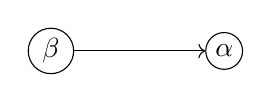
\begin{tikzpicture}[scale=1, every node/.style={circle,draw,inner sep=2pt}]
        \node (b) at (0,0) {\(\beta\)};
        \node (a) at (2.2,0) {\(\alpha\)};
        \draw[->] (b) -- (a);
    \end{tikzpicture}
\end{center}

Una pagina è importante se molti parlano di lei; è ancora più importante se chi parla di lei è a sua volta importante; l'importanza ricevuta da una pagina viene però distribuita tra tutti i suoi link uscenti.

Per esempio, nel grafo seguente, la pagina \(a\) riceve link da più pagine; la pagina \(b\) è importante perché riceve un link da \(a\), e \(a\) ha pochi link uscenti.

\begin{center}
    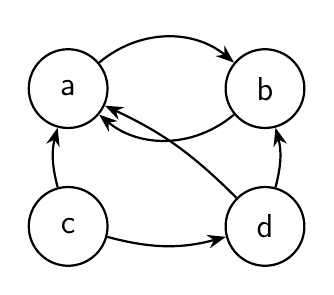
\begin{tikzpicture}[scale=0.5]
        \begin{scope}[every node/.style={draw, circle, thick, minimum size=1cm, font=\sffamily\large}]
            \node (a) at (0,3.5) {a};
            \node (b) at (5,3.5) {b};
            \node (c) at (0,0) {c};
            \node (d) at (5,0) {d};
        \end{scope}
        \begin{scope}[every path/.style={->, >=Stealth, thick}]
            \draw (a) to[bend left=40] (b);
            \draw (b) to[bend left=40] (a);
            \draw (c) to[bend left=15] (a);
            \draw (c) to[bend right=15] (d);
            \draw (d) to[bend right=15] (b);
            \draw (d) to[bend right=10] (a);
        \end{scope}
    \end{tikzpicture}
\end{center}

Numeriamo tutte le pagine del Web da \(1\) a \(N\), con \(N\) molto grande. Se \(L_\beta\) è il numero di link uscenti dalla pagina \(\beta\), la regola diventa
\[
    I(\alpha)
    =
    \sum_{\beta\to\alpha}\frac{I(\beta)}{L_\beta}.
\]
Questa formula dice che non si può calcolare una singola importanza isolatamente: tutte le importanze sono accoppiate e vanno calcolate simultaneamente.

\begin{snippetdefinition}{Matrice dei link}
    Definiamo la matrice \(A=(a_{\alpha\beta})\) ponendo
    \[
        a_{\alpha\beta}
        =
        \begin{cases}
            0, & \text{se } \beta \text{ non ha un link verso } \alpha,\\
            \dfrac1{L_\beta}, & \text{se } \beta \text{ ha un link verso } \alpha.
        \end{cases}
    \]
    Allora il vettore delle importanze \(I=(I(1),\ldots,I(N))^T\) deve soddisfare
    \[
        I=AI.
    \]
    Inoltre vogliamo
    \[
        I(\alpha)\geq 0,
        \qquad
        \sum_{\alpha=1}^N I(\alpha)=1.
    \]
\end{snippetdefinition}

La matrice \(A\) è enorme, perché \(N\) è dell'ordine delle pagine del Web, ma è anche estremamente sparsa: ogni pagina contiene solo pochi link rispetto a \(N\).

\subsection{Metodo delle potenze per il ranking}

Il primo algoritmo naturale è il metodo delle potenze applicato ad \(A\):
\[
    I^{(0)}=\frac1N
    \begin{pmatrix}
        1\\
        \vdots\\
        1
    \end{pmatrix},
    \qquad
    I^{(k+1)}=AI^{(k)}.
\]
Se esiste
\[
    \lim_{k\to\infty}I^{(k)}=I^*,
\]
allora il vettore \(I^*\) soddisfa
\[
    I^*=AI^*.
\]
Quindi \(I^*\) è un autovettore associato all'autovalore \(1\). In questo contesto non serve una precisione altissima: l'obiettivo è soprattutto ordinare le pagine per importanza.

\subsection{Pagine senza link uscenti}

\begin{snippetexample}{Pagina senza link uscenti}
    Consideriamo due pagine, con un solo link \(1\to 2\) e nessun link uscente da \(2\):

    \begin{center}
        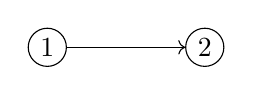
\begin{tikzpicture}[scale=1, every node/.style={circle,draw,inner sep=2pt}]
            \node (one) at (0,0) {\(1\)};
            \node (two) at (2,0) {\(2\)};
            \draw[->] (one) -- (two);
        \end{tikzpicture}
    \end{center}

    La matrice dei link è
    \[
        A=
        \begin{pmatrix}
            0&0\\
            1&0
        \end{pmatrix}.
    \]
    Questa matrice non è stocastica per colonne: la seconda colonna è nulla. Inoltre \(1\) non è autovalore di \(A\), quindi il metodo delle potenze non può convergere a un autovettore di importanza normalizzato.
\end{snippetexample}

Il rimedio è aggiungere teletrasporto sulle colonne nulle. Sia
\[
    u=\frac1N
    \begin{pmatrix}1\\ \vdots\\ 1
    \end{pmatrix}
\]
e sia \(z\in\realnumbers^N\) definito da
\[
    z_j=
    \begin{cases}
        1, & \text{se la colonna } j \text{ di } A \text{ è nulla},\\
        0, & \text{altrimenti}.
    \end{cases}
\]
Definiamo
\[
    A'=A+uz^T.
\]
In questo modo ogni colonna nulla viene sostituita con la distribuzione uniforme \(u\).

\begin{snippettheorem}{Autovalore principale per matrici stocastiche per colonne}
    La matrice \(A'\) è stocastica per colonne. Di conseguenza \(1\) è autovalore di \(A'\) e
    \[
        \rho(A')=1.
    \]
\end{snippettheorem}

\begin{snippetproof}{}
    Per costruzione ogni colonna di \(A'\) ha elementi non negativi e somma pari a \(1\). Dunque
    \[
        \|A'\|_1=1.
    \]
    Ne segue che
    \[
        \rho(A')\leq \|A'\|_1=1.
    \]
    D'altra parte, se \(\mathbf 1=(1,
    \ldots,1)^T\), la condizione di stocasticità per colonne equivale a
    \[
        \mathbf 1^T A'=\mathbf 1^T.
    \]
    Quindi \(1\) è autovalore di \((A')^T\), e dunque anche di \(A'\). Pertanto \(\rho(A')\geq 1\), e concludiamo che \(\rho(A')=1\).
\end{snippetproof}

\subsection{Oscillazioni e periodicità}

Anche se la matrice è stocastica per colonne, il metodo delle potenze può non convergere. Per esempio, con due pagine che si puntano a vicenda,

\begin{center}
    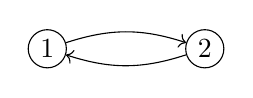
\begin{tikzpicture}[scale=1, every node/.style={circle,draw,inner sep=2pt}]
        \node (one) at (0,0) {\(1\)};
        \node (two) at (2,0) {\(2\)};
        \draw[->,bend left=18] (one) to (two);
        \draw[->,bend left=18] (two) to (one);
    \end{tikzpicture}
\end{center}

si ottiene
\[
    A=
    \begin{pmatrix}
        0&1\\
        1&0
    \end{pmatrix}.
\]
Gli autovalori sono \(1\) e \(-1\). La presenza dell'autovalore \(-1\), di modulo \(1\), può produrre oscillazioni e impedire la convergenza del metodo delle potenze.

\subsection{Teletrasporto e convergenza del PageRank}

Brin e Page introdussero un parametro di teletrasporto. Sia \(c\in[0,1)\), tipicamente
\[
    c\simeq 0.85.
\]
Definiamo
\[
    A_c=cA'+(1-c)\frac1N\mathbf 1\mathbf 1^T.
\]
La matrice
\[
    \frac1N\mathbf 1\mathbf 1^T
\]
è la matrice le cui colonne sono tutte uguali alla distribuzione uniforme. Quindi \(A_c\) è combinazione convessa di matrici stocastiche per colonne e, a sua volta, è stocastica per colonne.

\begin{snippettheorem}{Spettro della matrice con teletrasporto}
    La matrice \(A_c\) ha autovalore \(1\). Inoltre, se \(\lambda\neq 1\) è un autovalore di \(A_c\), allora
    \[
        |\lambda|\leq c<1.
    \]
    Di conseguenza il metodo delle potenze applicato ad \(A_c\) converge a un vettore stocastico \(I^*\).
\end{snippettheorem}

\begin{snippetproof}{}
    Poiché \(A_c\) è stocastica per colonne, \(1\) è autovalore. Studiamo gli altri autovalori.

    Poniamo
    \[
        E=\frac1N\mathbf 1\mathbf 1^T.
    \]
    Per \(\lambda\notin \sigma(cA')\), usando la formula del determinante di una perturbazione di rango uno,
    \begin{align*}
        p_{A_c}(\lambda)
        &=\det(A_c-\lambda I)\\
        &=\det\left(cA'-\lambda I+(1-c)E\right)\\
        &=\det(cA'-\lambda I)
        \left(
            1+\frac{1-c}{N}\mathbf 1^T(cA'-\lambda I)^{-1}\mathbf 1
        \right).
    \end{align*}
    Siccome \(A'\) è stocastica per colonne,
    \[
        \mathbf 1^T A'=\mathbf 1^T.
    \]
    Quindi
    \[
        \mathbf 1^T(cA'-\lambda I)
        =(c-
        \lambda)\mathbf 1^T.
    \]
    Da cui
    \[
        \mathbf 1^T(cA'-\lambda I)^{-1}
        =\frac1{c-
        \lambda}\mathbf 1^T.
    \]
    Pertanto
    \begin{align*}
        p_{A_c}(\lambda)
        &=p_{cA'}(\lambda)
        \left(
            1+
            \frac{1-c}{c-
            \lambda}
        \right)\\
        &=p_{cA'}(\lambda)
        \frac{1-
        \lambda}{c-
        \lambda}.
    \end{align*}
    Equivalentemente,
    \[
        (c-
        \lambda)p_{A_c}(\lambda)
        =(1-
        \lambda)p_{cA'}(\lambda).
    \]
    L'identità, ottenuta inizialmente fuori da un insieme finito, vale come identità polinomiale per continuità.

    Se gli autovalori di \(A'\) sono
    \[
        1,\mu_2,
        \ldots,
        \mu_N,
    \]
    con \(|\mu_j|\leq 1\), allora gli autovalori di \(A_c\) sono
    \[
        1,c\mu_2,
        \ldots,c\mu_N.
    \]
    Dunque ogni autovalore diverso da \(1\) ha modulo minore o uguale a \(c\). Poiché \(c<1\), il metodo delle potenze converge al vettore di PageRank \(I^*\), cioè al vettore stocastico che soddisfa
    \[
        A_c I^*=I^*.
    \]
\end{snippetproof}

\pagebreak

\section{Esercizi e problemi svolti}

\begin{snippetexercise}{}
    Sia \(\alpha \geq 1\) reale e consideriamo la matrice
    \[
        A_n(\alpha) =
        \begin{pmatrix}
            \alpha & 1 & 1 & \cdots & 1 \\
            1 & \alpha & 1 & \cdots & 1 \\
            1 & 1 & \alpha & \cdots & 1 \\
            \vdots & \vdots & \ddots & \ddots & 1 \\
            1 & 1 & \cdots & 1 & \alpha
        \end{pmatrix}
    \]
    e
    \[
        B_n(\alpha) =
        \begin{pmatrix}
            \alpha & -1 & -1 & \cdots & -1 \\
            1 & \alpha & -1 & \cdots & -1 \\
            1 & 1 & \alpha & \cdots & -1 \\
            \vdots & \vdots & \ddots & \ddots & -1 \\
            1 & 1 & \cdots & 1 & \alpha
        \end{pmatrix}
    \]
    \begin{enumerate}
        \item Si consideri nella maniera più precisa possibile lo spettro di \(A_n\)
            e \(B_n\).
        \item In particolari, si studi per quale \(\alpha\)
            le matrici risultano invertibili.
            sono invertibili?
        \item Indicato con \(e_1\) il primo vettore
            della base canonica, è vero che \(A_n^{(2)} + e_1e_1^T\) è definita positiva?
        \item È vero che \(A_n^{(1)} + e_1e_1^T\) è semidefinita positiva?
    \end{enumerate}
\end{snippetexercise}

\begin{snippetsolution}{}
    Cominciamo notando che \(A_n^*(\alpha) = A_n^T(\alpha) = A_n(\alpha)\)
    quindi è Hermitiana e il suo spettro è reale.
    Possiamo notare che \(X_n + \alpha I_n = B_n(\alpha)\)
    dove
    \[
        X_n =
        \begin{pmatrix}
            0 & -1 & \cdots & -1 \\
            1 & 0 & \cdots & -1 \\
            \vdots & \vdots & \ddots & \vdots \\
            1 & 1 & \cdots & 0
        \end{pmatrix}
    \]
    % TODO definire pure Y_n e scrivere meglio
    Moltiplicando \(iX_n = Y_n\) diventa hermitiana \(Y_n^*  = Y_n\).
    In generale se moltiplichiamo una matrice per qualcosa, pure i suoi valori vengono moltiplicati per tale quantità.
    Quindi \(Y_n x = \lambda x\) con \(\lambda \in \realnumbers\)
    ci porta a dire che \(X_n\) può avere solo autovalori immaginari puri.
    Se \(X_n v = \lambda v\),
    allora
    \begin{align*}
        (\alpha I + X_n)v &= \alpha v + X_n v = (\alpha + \lambda)v
    \end{align*}
    quindi gli autovalori di \(B_n(\alpha)\)
    sono della forma \(\alpha + i\beta\) con \(\beta \in \realnumbers\).
    Per struttura degli autovalori, siccome non toccano mai lo zero, sono tutte invertibili.
    Consideriamo il caso \(\alpha = 1\). In tal caso la matrice \(A_n\) è singolare,
    quindi non è invertibile. Consideriamo \(\alpha > 1\).
    Abbiamo
    \begin{align*}
        A_n(\alpha) &= (\alpha - 1)I_n +
        \begin{pmatrix}
            1 & 1 & \cdots & 1 \\
            1 & 1 & \cdots & 1 \\
            \vdots & \vdots & \ddots & \vdots \\
            1 & 1 & \cdots & 1
        \end{pmatrix} \\
        &=  (\alpha - 1) I_n +
        \begin{pmatrix}
            1 \\ 1 \\ \vdots \\ 1
        \end{pmatrix}
        \begin{pmatrix}
            1 & 1 & \cdots & 1
        \end{pmatrix}
        = (\alpha -1)I_n + e_1e_1^T
    \end{align*}
    Il primo termine è definito positivo,
    mentre il secondo è la matrice di uni che ha rango \(1\),
    quindi la si può scrivere come prodotto di colonna per riga.
    Vogliamo verificare che la forma quadratica sia definita positiva,
    cioè studiamo \(x^* A_n(\alpha)x\). Sappiamo che
    \begin{align*}
        x^*A_n(\alpha)x &= \underbrace{x(\alpha - 1)I_n x}_{> 0} + xe_1e_1^T x \\
        &= \underbrace{x(\alpha - 1)I_n x}_{> 0} + (e_1^T x)^2
    \end{align*}
    e quindi abbiamo un termine positivo psommato ad una quantità non-negativa.
    Scomponiamo ora invece l'altra matrice come
    \begin{align*}
        B_n(\alpha) = \alpha I_n + V_n
    \end{align*}
    dove abbiamo già verificato che \((iV_n)^* = i V_n = -i V_n\),
    quindi otteniamo che \(V_n\) è anti-Hermitiana, cioè \(V_n^* = -V_n\).
\end{snippetsolution}

\begin{snippetdefinition}{Matrice di Vandermonde generalizzata}
    Siano \(x_0, x_1, \cdots, x_n \in \complexnumbers\)
    e siano \(p_0, p_1, \cdots, p_n \in \complexnumbers[x]\), \(n+1\) polinomi linearmente indipendenti.
    La \emph{matrice di Vandermonde generalizzata è definita come}
    \[
        W_n \triangleq (p_k(x_j))_{j,k=0}^n \in \matrices_{n+1}(\complexnumbers)
    \]
\end{snippetdefinition}

\begin{snippetexercise}{Matrice di Vandermonde generalizzata}
    Consideriamo una matrice di Vandermonde generalizzata \(W_n\).
    Sia \[
        K_n = \max_{0 \leq k \leq n} \{ \deg (p_k) \} % polynomialdeg
    \]
    \begin{enumerate}
        \item Si dimostri che \(\det W_n \neq 0\)
            implica che \(x_0, x_1, \cdots, x_n\) sono a due a due distinti.
        \item Se \(K_n = n\) e \(x_0, x_1, \cdots, x_n\)
            sono a due a due distinti è vero che \(\det W_n \neq 0\)? (Unisolvenza)
        \item Se \(K_n > n\) e \(x_0, x_1, \cdots, x_n\)
            sono a due a due distinti è ancora vero che si ha unisolvenza,
            ovvero \(\det W_n \neq 0\)?.
    \end{enumerate}
\end{snippetexercise}

\begin{snippetsolution}{Matrice di Vandermonde generalizzata}
    \todo
\end{snippetsolution}

\begin{snippetexercise}{}
    Sia \(n\) grande.
    Siano dati \(2n\) numeri positivi \(x_j, y_j\)
    per \(j \in \{1, \cdots, n\}\) tali che
    \[
        x_jy_j > \frac12, \quad \forall j \in \{1, \cdots, n\}
    \]
    Siano \(v_1, \cdots, v_n \in \realnumbers^2\)
    con \(v_j =
        \begin{pmatrix}x_j \\ y_j
    \end{pmatrix}\)
    e \(j \in \{1, \cdots, n\}\) e si consideri \(A \in \matrices_n(\realnumbers)\) tale che
    \[
        A_{j,k} = 1, \quad j\neq k, k,j \in \{1, \cdots, n\}, \quad A_{j,j} = ||v_j||_2
    \]
    Sia \(B \in \matrices_n(\realnumbers)\)
    la matrice tridiagonale simmetrica con \(B_{j,j} = 2\)
    per \(j \in \{1, \cdots, n\}\) e \(B_{j,j\pm 1} = 1\)
    per \(j \in \{1, \cdots, n-1\}\).
    Si consideri \(C \in \matrices_{2n}(\realnumbers)\)
    data da \[
        C =
        \begin{pmatrix}
            A & A^2 - x_1A \\
            0 & B
        \end{pmatrix}
    \]
    \begin{enumerate}
        \item Si dimostri che \(A,B,C\) sono invertibili.
        \item Si localizzi lo spettro di \(C\) nel modo migliore possibile.
        \item Si dimostri che la fattorizzazione \(LU\) di \(C\) esiste unica ovvero \(C\)
            fortemente non singolare.
        \item Si dimostri la convergenza del metodo di Gauss-Seidel applicato ad un sistema \(Cx=b\) con \(b \in \realnumbers^{2n}\).
        \item Si dimostri che \(f(A), f(B), f(C)\) sono invertibili con \(f(x) = 1 - x + x^{31}\).
            È vero che tutti gli autovalori \(f(C)\) sono positivi?
    \end{enumerate}
\end{snippetexercise}

\begin{snippetsolution}{}
    \begin{enumerate}
        \item TODO
        \item TODO
        \item TODO
        \item La matrice non è Hermitiana ed è difficile definire se è a predominanza diagonale, probabilmente no.
            Nessuno dei teoremi di condizioni sufficienti ci aiuta.
            Abbiamo il metodo di Gauss-Seidel \(Z u = w\).
            Scegliamo lo splitting \(M\) la parte inferiore di \(Z\) e \(-N\) la parte superiore stretta.
            Consideriamo \(C\). Allora la sua parte triangolare inferiore, è composta da due blocchi di \(0\) (alto a destra e basso a sinistra)
            e due blocchi con rispettivamente le parti triangolari inferiori di \(A\) e \(B\).
            Invece, la triangolare superiore stretta di \(C\) ha diagonale tutta nulla, il blocco in basso a sinistra nullo,
            il primo e quarto blocco contenenti la parte triangolare superiore stretta di \(A\) e \(B\) rispettivamente,
            e il secondo blocco pieno di elementi.
            \[
                M=
                \begin{pmatrix}
                    \operatorname{tril}(A) & 0\\
                    0 & \operatorname{tril}(B)
                \end{pmatrix},
                \qquad
                N=
                \begin{pmatrix}
                    -\operatorname{triu}(A,1) & -(A^2-x_1A)\\
                    0 & -\operatorname{triu}(B,1)
                \end{pmatrix}.
            \]
            Quindi il prodotto è composto come
            \[
                \begin{pmatrix}
                    P_{\text{GS}}(A) & \ast \\
                    0 & P_{\text{GS}}(B)
                \end{pmatrix}
            \]
            Abbiamo che
            \[
                \sigma(P_{\text{GS}}(C)) = \sigma(P_{\text{GS}}(A)) \union \sigma(P_{\text{GS}}(B))
            \]
            Questo è dato dal fatto che il determinante della matrice a blocchi è il determinante di \(A\)
            per quello di \(B\), quindi il polinomio caratteristico è il prodotto dei due polinomi carateristici.
            Sapendo che sono entrambe definite positive
            \[
                \rho(P_{\text{GS}}(C)) = \max\{\rho(P_{\text{GS}}(A)), \rho(P_{\text{GS}}(B))\} < 1
            \]
            Quindi vale la tesi.
        \item Abbiamo la scomposizione di Jordan \(X = TJT^{-1}\)
            \[
                f(X) = I - X + X^3 = T(i- J + J^{31})T^{-1}
            \]
            Il polinomio sulla matrice diventa il polinomio sui blocchi di Jordan.
            Quando facciamo le potenze, sulle diagonali rimangono le potenze degli autovalori mentre
            fuori comincia a salire la triangolare superiore.
            Quindi gli autovalori di \(\sigma(f(X)) = f(\sigma(X))\).
            Studiamo la funzione notando che su \([0,+\infty)\)
            è strettamente positiva, e quindi le matrici sono ancora invertibili.
    \end{enumerate}
\end{snippetsolution}

\begin{snippetexercise}{}
    Sia \(A \in \matrices_n(\realnumbers)\)
    con \(n\) pari, \(a,b, c>0\) e \(a>b\). Definiamo
    \[
        \left(A\right)_{j,k} =
        \begin{cases}
            a + c & j=k \\
            a & (j+k) \equiv 0 \pmod{2} \land j \neq k \\
            b & (j+k) \equiv 1 \pmod{2}
        \end{cases}
    \]
    \begin{enumerate}
        \item Caratterizzare lo spettro nel modo migliroe possibile;
        \item Dimostrare che il metodo di Gauss-Seidel è convergente
            se applicato ad un sistema lineare \(Ax = b\).
    \end{enumerate}
\end{snippetexercise}

\begin{snippetsolution}{}
    Abbiamo la forma della matrice
    \begin{align*}
        A &=
        \begin{pmatrix}
            a+c & b   & a   & b   & a   & \cdots & b \\
            b   & a+c & b   & a   & b   & \cdots & a \\
            a   & b   & a+c & b   & a   & \cdots & b \\
            b   & a   & b   & a+c & b   & \cdots & a \\
            a   & b   & a   & b   & a+c & \cdots & b \\
            \vdots & \vdots & \vdots & \vdots & \vdots & \ddots & \vdots \\
            b   & a   & b   & a   & b   & \cdots & a+c
        \end{pmatrix} \\
        &= cI_n + b \underbrace{
            \begin{pmatrix}
                0 & 1   & 0   & 1   & 0   & \cdots & 1 \\
                1   & 0 & 1   & 0   & 1   & \cdots & 0 \\
                0   & 1   & 0 & 1   & 0   & \cdots & 1 \\
                1   & 0   & 1   & 0 & 1   & \cdots & 0 \\
                0   & 1   & 0   & 1   & 0 & \cdots & 1 \\
                \vdots & \vdots & \vdots & \vdots & \vdots & \ddots & \vdots \\
                1   & 0   & 1   & 0   & 1   & \cdots & 0
        \end{pmatrix}}_{E}
        + a \underbrace{
            \begin{pmatrix}
                1   & 0   & 1   & 0   & \cdots & 1 & 0 \\
                0 & 1   & 0   & 1   & \cdots & 0 & 1 \\
                1   & 0 & 1   & 0   & \cdots & 1 & 0 \\
                0   & 1   & 0 & 1   & \cdots & 0 & 1 \\
                1   & 0   & 1   & 0 & \cdots & 1 & 0 \\
                \vdots & \vdots & \vdots & \vdots & \vdots & \ddots & \vdots \\
                0   & 1   & 0   & 1   & \cdots & 0 & 1
        \end{pmatrix}}_{F}
    \end{align*}
    Sicuramente un generico autovalore
    \[
        \lambda(A) = c + \lambda(bF + aE)
    \]
    (Perché e quando si può fare?).
    Notiamo che \(F\) ed \(E\) hanno solamente due righe uguali, quindi il logo
    rango è \(\leq 2\), ma le due righe sono chiaramente indipendenti
    quindi il rango è precisamente \(2\). Abbiamo quindi che \(\operatorname{rank} (bF) = \operatorname{rank} (aE) = 2\).
    Quindi la matrice completa ha al massimo rango \(4\). Quindi,
    \(A\) ha autovalore \(c\) con molteplicità almeno \(n-4\), mentre gli altri \(4\)
    autovalori dobbiamo ancora trovarli.
    La matrice è reale e simmetrica e Hermitiana quindi diagonalizzabile,
    quindi le molteplicità algebrichde e geometriche coincidono.
    Siano
    \[
        f =
        \begin{pmatrix}
            0 \\ 1 \\ 0 \\ \vdots \\ 1
        \end{pmatrix} \in \{0,1\}^n,
        g =
        \begin{pmatrix}
            0 \\ 1 \\ 0 \\ \vdots \\ 1
        \end{pmatrix}\in \{0,1\}^n
    \]
    da cui trovimo \(E = gg^T + ff^T\) e \(F = gf^T + fg^T\).
    Allora, la matrice
    \begin{align*}
        bF + aE &= b\left(gf^T + fg^T\right)
        + a\left(gg^T + ff^T\right) \\
        &= g\left(
            bf^T + ag^T
        \right) + f\left(
            bg^T + af^T
        \right)
    \end{align*}
    Ma da questa decomposizione deduciamo che il rango di
    \(bF + aE\) è precisamente \(\leq 2\), in quanto possiamo generare tutto come combinazione di due vettori.
    In realtà è precisamente \(2\) perché possiamo trovare
    un minore di testa principale il cui rango è al massimo due
    (cioè il primo minore di testa principale \(2\times 2\))
    quindi \(\operatorname{rank}(bF + aE)=2\).
    Quindi, \(A\) ha autovalore \(c\) con molteplicità almeno \(n-2\), e altri \(2\)
    autovalori.
    Adesso scriviamo
    \begin{align*}
        bF+aE &=
        \left[
            \begin{array}{c|c}
                &  \\
                f & g \\
                &
            \end{array}
        \right]
        \left[
            \begin{array}{c}
                bg^T+af^T \\ \hline
                bf^T+ag^T
            \end{array}
        \right]
    \end{align*}
    Questa scomposizione funziona più in generale.
    Applicando il teorema di commutazione dello spettro per moltiplicazione di matrici,
    invertiamo l'ordine e calcoliamo gli autovalori
    della matrice risultante, che sono i due autovalori non banali rimanenti. Abbiamo quindi
    \begin{DispWithArrows*}
        \left[
            \begin{array}{c}
                bg^T+af^T \\ \hline
                bf^T+ag^T
            \end{array}
        \right]
        \left[
            \begin{array}{c|c}
                &  \\
                f & g \\
                &
            \end{array}
        \right]
        &=
        \begin{pmatrix}
            a||f||_2^2 & b||g||_2^2 \\
            b||f||_2^2 & a||g||_2^2
        \end{pmatrix} \Arrow{\(n\) è pari} \\
        &= \frac n2
        \begin{pmatrix}
            a & b \\ b & a
        \end{pmatrix}
    \end{DispWithArrows*}
    Quindi gli autovalori di \(A\) sono \(c\)
    con molteplicità \(n-2\), e \(c + \frac n2(a\pm b)\) con molteplicità \(1\).
    È diagonalizzabile in quanto \(a > b\), quindi il metodo di Gauss-Seidel converge.
\end{snippetsolution}

\pagebreak

Formula generale dal complemento di Schur. Se \(E\) è invertibile allora
\[
    \begin{pmatrix}
        E & F \\
        G & H
    \end{pmatrix}
    =
    \begin{pmatrix}
        I & 0 \\
        GE^{-1} & I
    \end{pmatrix}
    \begin{pmatrix}
        E & 0 \\
        0 & H-GE^{-1}F
    \end{pmatrix}
    \begin{pmatrix}
        I & E^{-1}F \\
        0 & I
    \end{pmatrix}
\]
con matrici quadrate.

\begin{snippetexercise}{Spettro, soluzione veloce e convergenza per una matrice a blocchi}
    Sia
    \[
        A =
        \begin{pmatrix}
            B_1 & C \\
            0 & B_2
        \end{pmatrix}
    \]
    una matrice a blocchi, con \(m_1, m_2 \in \naturalnumbers^+\), \(m_1, m_2 \geq 2\),
    \(n=m_1+m_2\), così da definire
    \(B_1 \in \matrices_{m_1}(\realnumbers)\)
    e \(B_2 \in \matrices_{m_2}(\realnumbers)\), e
    \(C \in \matrices_{m_1 \times m_2}(\realnumbers)\) tale che
    \[
        (C)_{i,j} = 1 + i, \quad 1 \leq i \leq m_1, \quad 1 \leq j \leq m_2
    \]
    Le matrici hanno forma
    \[
        B_1 =
        \begin{pmatrix}
            3 & - 1 & & & \\
            -1 & 3 & -1 & & \\
            & -1 & \ddots & \ddots & \\
            & & \ddots & \ddots & -1 \\
            & & & -1 & 3
        \end{pmatrix}, \quad
        B_2 =
        \begin{pmatrix}
            2 & \alpha_{1} & & & \\
            \delta_1 & 2 & \alpha_{2} & & \\
            & \delta_2 & \ddots & \ddots &  \\
            & & \ddots & \ddots & \alpha_{m_2-1} \\
            & & & \delta_{m_2-1} & 12
        \end{pmatrix}
    \]
    dove la diagonale di \(B_2\) è tutta costante tranne l'ultimo elemento, e gli elementi sono definiti come
    \[
        \alpha_j = 1 + \frac{1}{9 + j}, \quad
        \frac{1}{10} \leq \delta_j \leq \frac15, \quad j=1,\cdots,m_2-1.
    \]
    \begin{enumerate}
        \item Studiare lo spettro di \(A\);
        \item Determinare se \(\exists_{=1} \lambda\) autovalore tale che \(\lambda = \rho(A)\);
        \item Determinare se \(A\) è invertibile;
        \item Trovare un algoritmo veloce per risolvere \(Ax=b\) e calcolarne il costo computazionale;
        \item Mostrare la convergenza. Qual è il \(k\) minimo?
    \end{enumerate}
\end{snippetexercise}

\begin{snippetsolution}{}
    \begin{enumerate}
        \item Dalla forma della matrice sappiamo che \[
                \sigma(A) = \sigma(B_1) \union \sigma(B_2)
            \]
            Lo si vede usando la forma triangolare a blocchi.
            Studiamo quindi separatamente questi spettri. I dischi di Gershgorin di \(B_1\) sono
            \begin{align*}
                D_1 = D_{m_1} &= \{ z \in \complexnumbers \suchthat |z-3| \leq 1\} = [2,4] \\
                D_i &= \{ z \in \complexnumbers \suchthat |z-3| \leq 2\} = [1,5], \quad 1 < i < m_1 \\
            \end{align*}
            siccome la matrice è simmetrica, quindi gli autovalori sono reali.
            Allora abbiamo che \(\sigma(B_1) \subseteq [1,5]\).
            La matrice \(B_1\) è irriducibile in quanto il suo grafo associato è fortemente connesso (esempio con \(m_1 = 6\)):
            \begin{center}
                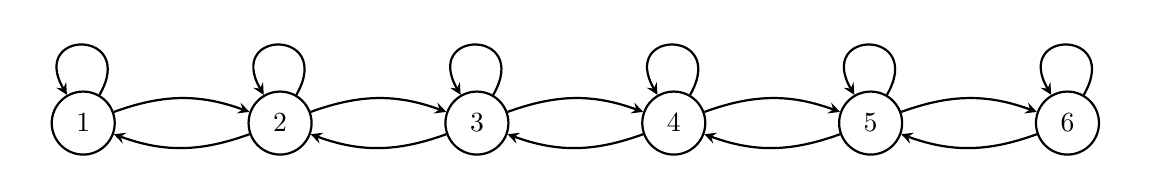
\begin{tikzpicture}[>=stealth, node distance=2cm]
                    \node[circle, draw, thick, minimum size=8mm] (1) at (0,0) {1};
                    \node[circle, draw, thick, minimum size=8mm] (2) at (2.5,0) {2};
                    \node[circle, draw, thick, minimum size=8mm] (3) at (5,0) {3};
                    \node[circle, draw, thick, minimum size=8mm] (4) at (7.5,0) {4};
                    \node[circle, draw, thick, minimum size=8mm] (5) at (10,0) {5};
                    \node[circle, draw, thick, minimum size=8mm] (6) at (12.5,0) {6};

                    \foreach \i in {1,2,3,4,5,6} {
                        \draw[->, thick] (\i) to[out=60, in=120, looseness=6] (\i);
                    }

                    \foreach \i/\j in {1/2, 2/3, 3/4, 4/5, 5/6} {
                        \draw[->, thick] (\i) to[bend left=20] (\j);
                        \draw[->, thick] (\j) to[bend left=20] (\i);
                    }
                \end{tikzpicture}
            \end{center}
            Per il terzo teorema di Gershgorin, se un autovalore fosse \(1\) o \(5\)
            dovrebbe stare sul bordo di tutti i dischi, ma \(1,5 \notin D_1 = D_{m_1}\).
            Quindi \(\sigma(B_1) \subseteq (1,5)\). In realtà, essendo \(B_1\) tridiagonale di Toeplitz,
            \[
                \sigma(B_1) = \left\{3 - 2\cos\left(\frac{k\pi}{m_1+1}\right) \suchthat k=1,\cdots,m_1\right\}.
            \]
            Studiamo ora lo spettro di \(B_2\).
            Studiamo lo spettro di \(\tilde B = D B_2 D^{-1}\) con \(D\) diagonale invertibile, che tanto non cambia.
            Costruiamo la matrice \(D\) come
            \[
                D = \operatorname{diag}(d_1, \cdots, d_{m_2})
            \]
            con \[
                d_1 = 1, \quad \frac{d_{j+1}}{d_j} = \sqrt{
                    \frac{\alpha_j}{\delta_j}
                }
            \]
            Eseguendo il prodotto troviamo
            \[
                \tilde B =
                \begin{pmatrix}
                    2 & \alpha_1 \frac{d_1}{d_2} & & & \\
                    \delta_1 \frac{d_2}{d_1} & 2 & \alpha_2 \frac{d_2}{d_3} & & \\
                    & \delta_2 \frac{d_3}{d_2} & \ddots & \ddots & \\
                    & & \ddots & 2 & \alpha_{m_2-1} \frac{d_{m_2-1}}{d_{m_2}} \\
                    & & & \delta_{m_2-1} \frac{d_{m_2}}{d_{m_2-1}} & 12
                \end{pmatrix}
                =
                \begin{pmatrix}
                    2 & \gamma_1 & & & \\
                    \gamma_1 & 2 & \gamma_2 & & \\
                    & \gamma_2 & \ddots & \ddots & \\
                    & & \ddots & 2 & \gamma_{m_2-1} \\
                    & & & \gamma_{m_2-1} & 12
                \end{pmatrix}
            \]
            dove \(\gamma_j = \sqrt{\alpha_j\delta_j}\). Abbiamo precisamente scelto i valori \(d_j\) per forzare una matrice Hermitiana.
            Calcoliamo ora i dischi di Gershgorin di questa matrice:
            \begin{align*}
                D_1 &= \left[2 - \gamma_1, 2 + \gamma_1\right] \\
                D_i &= \left[2 - (\gamma_{i-1} + \gamma_i), 2 + (\gamma_{i-1} + \gamma_i)\right], \quad 1 < i < m_2 \\
                D_{m_2} &= \left[12 - \gamma_{m_2 - 1}, 12 + \gamma_{m_2 - 1}\right]
            \end{align*}
            I primi \(m_2-1\) dischi stanno tutti vicino a \(2\), mentre l'ultimo sta vicino a \(12\).
            Diamo un bound \[
                \frac1{10} \left(1 + \frac{1}{9+j}\right) \leq
                \alpha_j \delta_j \leq \frac15 \left(1 + \frac{1}{9+j}\right)
                \leq \frac{11}{50}
            \]
            Vogliamo anche stimare la somma \[
                \sqrt{\alpha_{i-1}\delta_{i-1}} + \sqrt{\alpha_i \delta_i}
                \leq \sqrt{
                    \frac{i + 9}{i + 8}\frac15
                } + \sqrt{
                    \frac{i + 10}{i + 9}\frac15
                } \leq \sqrt{\frac{11}{50}} + \sqrt{\frac{12}{55}}
            \]
            dove il massimo si ottiene per \(i=2\). Quindi, \[
                \sigma(B_2) = \sigma(\tilde B) \subseteq
                \left[
                    2 - \left(\sqrt{\frac{11}{50}} + \sqrt{\frac{12}{55}}\right),
                    2 + \sqrt{\frac{11}{50}} + \sqrt{\frac{12}{55}}
                \right]
                \union
                \left[
                    12 - \sqrt{\frac{11}{50}},
                    12 + \sqrt{\frac{11}{50}}
                \right].
            \]
            Il raggio più grande del secondo termine avviene per \(m_2 = 2\), così otteniamo una stima globale
            per qualsiasi grandezza, cioè raggio \(\sqrt{\sfrac{11}{50}}\).
            Questo può essere usato per controllare che l'ultimo cerchio sia isolato rispetto agli altri, cosa che è.
            Per il secondo teorema di Gershgorin, il primo intervallo contiene \(m_2-1\) autovalori di \(B_2\)
            e il secondo intervallo contiene un unico autovalore. Inoltre, per il terzo teorema di Gershgorin,
            siccome \(\tilde B\) è irriducibile, questo autovalore non può stare sul bordo del disco isolato.
        \item Per il secondo teorema di Gershgorin, c'è un unico autovalore \(\lambda_\ast\) di \(B_2\) vicino a \(12\).
            Inoltre,
            \[
                \lambda_\ast \geq 12 - \sqrt{\frac{11}{50}} > 5
            \]
            mentre gli autovalori di \(B_1\) stanno in \((1,5)\) e gli altri autovalori di \(B_2\) stanno
            nell'intervallo centrato in \(2\), che è contenuto in \((1,3)\). Quindi \(\rho(A)=\lambda_\ast\),
            e questo autovalore è unico.
        \item \(A\) è invertibile in quanto \(0 \notin \sigma(A)\).
        \item Siccome la matrice è a blocchi possiamo scrivere
            \[
                \begin{pmatrix}
                    B_1 & C \\ 0 & B_2
                \end{pmatrix}
                \begin{pmatrix}
                    Z \\ Y
                \end{pmatrix} =
                \begin{pmatrix}
                    b_1 \\ b_2
                \end{pmatrix}
            \]
            dove \(
                \begin{pmatrix}Z \\ Y
            \end{pmatrix}\) è un vettore a blocchi, quindi
            \(B_1 Z + CY = b_1\) e \(B_2 Y = b_2\). Dobbiamo quindi risolvere prima
            \(B_2 Y = b_2\), e poi \(B_1 Z = b_1 - CY\).
            Possiamo adoperare l'algoritmo di Thomas, cioè l'eliminazione di Gauss specializzata alle matrici tridiagonali,
            e poi risolvere con sostituzione all'indietro.
            Per una matrice tridiagonale \(r \times r\), la parte di eliminazione costa \(5(r-1)\) operazioni,
            mentre la sostituzione all'indietro costa \(1+3(r-1)\), quindi in totale \(8r - 7\) operazioni.
            Per \(CY\) non conviene costruire \(C\): siccome \(C_{i,j}=1+i\),
            \[
                (CY)_i = (1+i)\sum_{j=1}^{m_2}Y_j.
            \]
            Calcoliamo quindi \(s=\sum_{j=1}^{m_2}Y_j\) in \(m_2-1\) somme e poi \(b_1-CY\) in \(2m_1\) operazioni.
            Il costo totale è quindi \[
                (8m_2 - 7) + (m_2 - 1 + 2m_1) + (8m_1 - 7)
                = 10m_1 + 9m_2 - 15
            \]
            cioè \(\mathcal{O}(m_1+m_2)\).
        \item Sia \(A=M-N\) con \[
                M =
                \begin{pmatrix}
                    B_1 & 0 \\ 0 & B_2
                \end{pmatrix}, \quad
                N =
                \begin{pmatrix}
                    0 & -C \\ 0 & 0
                \end{pmatrix}
            \]
            Il metodo iterativo converge se
            \[
                \lim_{k \to +\infty} {(M^{-1} N)}^k = 0.
            \]
            Abbiamo \[
                M^{-1} =
                \begin{pmatrix}
                    B_1^{-1} & \\
                    & B_2^{-1}
                \end{pmatrix}, \quad
                M^{-1}N =
                \begin{pmatrix}
                    B_1^{-1} & 0 \\ 0 & B_2^{-1}
                \end{pmatrix}
                \begin{pmatrix}
                    0 & -C \\ 0 & 0
                \end{pmatrix} =
                \begin{pmatrix}
                    0 & -B_1^{-1}C \\ 0 & 0
                \end{pmatrix} = P
            \]
            Viene calcolato il quadrato della matrice di iterazione \(P\) per verificare dopo quanti passi il metodo converge esattamente,
            \[
                P^2 =
                \begin{pmatrix}
                    0 & -B_1^{-1}C \\
                    0 & 0
                \end{pmatrix}
                \begin{pmatrix}
                    0 & -B_1^{-1}C \\
                    0 & 0
                \end{pmatrix}=
                \begin{pmatrix}
                    0 & 0 \\
                    0 & 0
                \end{pmatrix}
            \]
            Quindi \(P\) è nilpotente, \(\rho(P)=0\), e il metodo converge. Siccome \(P \neq 0\), il \(k\) minimo è \(k=2\).
    \end{enumerate}
\end{snippetsolution}

\begin{snippetexercise}{}
    Siano \(n>3\) e
    \[
        B =
        \begin{pmatrix}
            2 & -1 & \cdots & -1 \\
            -\delta & 2 & & 0 \\
            \vdots & & \ddots & \\
            -\delta & 0 & & 2
        \end{pmatrix}
        \in \realnumbers^{n\times n},
        \qquad
        \frac{2}{n-1}<\delta<\frac{4}{n-1}.
    \]
    Studiare lo spettro di \(B\), risolvere il sistema \(Bx=b\), con
    \(b\in\realnumbers^n\), e stabilire la convergenza dei metodi di Jacobi e
    Gauss-Seidel.
\end{snippetexercise}

\begin{snippetsolution}{}
    Osserviamo anzitutto che i dischi di Gershgorin applicati direttamente alle
    righe non sono molto informativi: la prima riga ha raggio \(n-1\), quindi, per
    \(n\) grande, il disco corrispondente è molto ampio.

    Per migliorare la stima usiamo una similitudine diagonale. Sia
    \[
        D_r=\operatorname{diag}(1,r,\ldots,r),
        \qquad r>0.
    \]
    Allora \(B\) è simile a
    \[
        D_r^{-1}BD_r =
        \begin{pmatrix}
            2 & -r & \cdots & -r \\
            -\frac{\delta}{r} & 2 & & 0 \\
            \vdots & & \ddots & \\
            -\frac{\delta}{r} & 0 & & 2
        \end{pmatrix}.
    \]
    I raggi dei dischi di Gershgorin per righe sono
    \[
        R_1=(n-1)r,
        \qquad
        R_i=\frac{\delta}{r}, \quad i=2,\ldots,n.
    \]
    Bilanciamo i due raggi imponendo
    \[
        (n-1)r=\frac{\delta}{r},
        \qquad\text{cioè}\qquad
        r=\sqrt{\frac{\delta}{n-1}}.
    \]
    Con questa scelta,
    \[
        R_1=R_i=\sqrt{(n-1)\delta}.
    \]
    Poiché \(\delta<\frac{4}{n-1}\), si ha
    \[
        \sqrt{(n-1)\delta}<2.
    \]
    Quindi tutti gli autovalori stanno nel disco
    \[
        \left\{z\in\complexnumbers:|z-2|\leq \sqrt{(n-1)\delta}\right\},
    \]
    che non contiene \(0\). In particolare \(B\) è non singolare.

    Calcoliamo ora esattamente lo spettro. Scriviamo \(B\) come perturbazione di
    rango al più \(2\):
    \[
        B=2I_n+EF,
    \]
    dove
    \[
        E=
        \begin{pmatrix}
            0 & 1 \\
            1 & 0 \\
            \vdots & \vdots \\
            1 & 0
        \end{pmatrix}
        \in\realnumbers^{n\times 2},
        \qquad
        F=
        \begin{pmatrix}
            -\delta & 0 & \cdots & 0 \\
            0 & -1 & \cdots & -1
        \end{pmatrix}
        \in\realnumbers^{2\times n}.
    \]
    Infatti \(EF\) è la matrice con prima riga
    \[
        (0,-1,\ldots,-1),
    \]
    prima colonna, dalla seconda riga in poi,
    \[
        (-\delta,\ldots,-\delta)^T,
    \]
    e tutti gli altri elementi nulli.

    Gli autovalori non nulli di \(EF\) coincidono con quelli di \(FE\). Ora
    \[
        FE=
        \begin{pmatrix}
            0 & -\delta \\
            -(n-1) & 0
        \end{pmatrix}.
    \]
    Dunque
    \[
        \det(\lambda I_2-FE)
        =
        \lambda^2-(n-1)\delta,
    \]
    e quindi
    \[
        \sigma(FE)=
        \left\{
            -\sqrt{(n-1)\delta},
            \sqrt{(n-1)\delta}
        \right\}.
    \]
    Poiché \(EF\) ha rango al più \(2\), gli altri \(n-2\) autovalori sono nulli.
    Pertanto
    \[
        \sigma(EF)=
        \left\{
            -\sqrt{(n-1)\delta},
            \sqrt{(n-1)\delta},
            \underbrace{0,\ldots,0}_{n-2\text{ volte}}
        \right\}.
    \]
    Siccome \(B=2I_n+EF\), otteniamo
    \[
        \sigma(B)=
        \left\{
            2-\sqrt{(n-1)\delta},
            2+\sqrt{(n-1)\delta},
            \underbrace{2,\ldots,2}_{n-2\text{ volte}}
        \right\}.
    \]
    In particolare, usando ancora \(\delta<\frac{4}{n-1}\),
    \[
        2-\sqrt{(n-1)\delta}>0,
    \]
    quindi \(B\) è non singolare.

    Un modo equivalente per vedere l'autovalore \(2\) è considerare il sottospazio
    \[
        W=
        \left\{
            v\in\realnumbers^n:
            v_1=0,\
            \sum_{j=2}^{n}v_j=0
        \right\}.
    \]
    Se \(v\in W\), allora \(EFv=0\), quindi
    \[
        Bv=2v.
    \]
    Poiché \(\dim W=n-2\), l'autovalore \(2\) ha molteplicità almeno \(n-2\), e
    dalla decomposizione precedente sappiamo che la molteplicità è esattamente
    \(n-2\).

    Passiamo ora alla risoluzione del sistema \(Bx=b\). Le equazioni sono
    \begin{align*}
        2x_1-\sum_{j=2}^{n}x_j &= b_1, \\
        -\delta x_1+2x_j &= b_j,
        \qquad j=2,\ldots,n.
    \end{align*}
    Dalla seconda famiglia di equazioni ricaviamo
    \[
        x_j=\frac{b_j+\delta x_1}{2},
        \qquad j=2,\ldots,n.
    \]
    Poniamo
    \[
        s_b=\sum_{j=2}^{n}b_j.
    \]
    Allora
    \[
        \sum_{j=2}^{n}x_j
        =
        \sum_{j=2}^{n}\frac{b_j+\delta x_1}{2}
        =
        \frac{s_b+(n-1)\delta x_1}{2}.
    \]
    Sostituendo nella prima equazione,
    \begin{DispWithArrows*}
        2x_1-\frac{s_b+(n-1)\delta x_1}{2} &= b_1
        \Arrow{moltiplichiamo per \(2\)} \\
        4x_1-s_b-(n-1)\delta x_1 &= 2b_1
        \Arrow{raccogliamo \(x_1\)} \\
        \left(4-(n-1)\delta\right)x_1 &= 2b_1+s_b.
    \end{DispWithArrows*}
    Poiché \(4-(n-1)\delta>0\), otteniamo
    \[
        x_1=
        \frac{
            2b_1+\sum_{j=2}^{n}b_j
        }{
            4-(n-1)\delta
        }.
    \]
    Poi, per \(j=2,\ldots,n\),
    \[
        x_j=
        \frac{b_j+\delta x_1}{2}.
    \]
    Questa formula richiede soltanto il calcolo di una somma e poi il calcolo
    indipendente delle componenti \(x_j\), \(j=2,\ldots,n\). Bisogna però prestare
    attenzione alla stabilità numerica quando \(\delta\) è molto vicino a
    \(\frac{4}{n-1}\), perché il denominatore
    \[
        4-(n-1)\delta
    \]
    diventa piccolo.

    Studiamo infine Jacobi. La matrice diagonale di \(B\) è \(D=2I_n\), quindi la
    matrice di iterazione di Jacobi è
    \[
        P_J=
        \frac{1}{2}
        \begin{pmatrix}
            0 & 1 & \cdots & 1 \\
            \delta & 0 & \cdots & 0 \\
            \vdots & \vdots & \ddots & \vdots \\
            \delta & 0 & \cdots & 0
        \end{pmatrix}.
    \]
    Sul sottospazio
    \[
        W=
        \left\{
            v\in\realnumbers^n:
            v_1=0,\
            \sum_{j=2}^{n}v_j=0
        \right\}
    \]
    la matrice \(P_J\) è nulla. Rimane quindi da studiare l'azione sul sottospazio
    generato da \(e_1\) e dal vettore
    \[
        w=(0,1,\ldots,1)^T.
    \]
    Rispetto alla base \(\{e_1,w\}\), l'azione è descritta dalla matrice
    \[
        \begin{pmatrix}
            0 & \frac{n-1}{2} \\
            \frac{\delta}{2} & 0
        \end{pmatrix}.
    \]
    Quindi
    \[
        \sigma(P_J)=
        \left\{
            -\frac{1}{2}\sqrt{(n-1)\delta},
            \frac{1}{2}\sqrt{(n-1)\delta},
            \underbrace{0,\ldots,0}_{n-2\text{ volte}}
        \right\}.
    \]
    Il raggio spettrale è
    \[
        \rho(P_J)
        =
        \frac{1}{2}\sqrt{(n-1)\delta}.
    \]
    Poiché
    \[
        \delta<\frac{4}{n-1},
    \]
    segue che
    \[
        \rho(P_J)<1.
    \]
    Dunque il metodo di Jacobi converge.

    Per Gauss-Seidel, dalla forma delle equazioni, l'errore soddisfa
    \begin{align*}
        e_1^{(k+1)}
        &=
        \frac{1}{2}\sum_{j=2}^{n}e_j^{(k)}, \\
        e_i^{(k+1)}
        &=
        \frac{\delta}{2}e_1^{(k+1)}
        =
        \frac{\delta}{4}\sum_{j=2}^{n}e_j^{(k)},
        \qquad i=2,\ldots,n.
    \end{align*}
    Da qui si vede che la matrice di iterazione di Gauss-Seidel ha come unico
    autovalore eventualmente non nullo
    \[
        \frac{(n-1)\delta}{4}.
    \]
    Quindi
    \[
        \rho(P_{GS})
        =
        \frac{(n-1)\delta}{4}
        =
        \rho(P_J)^2.
    \]
    Ancora una volta, poiché \(\delta<\frac{4}{n-1}\), si ha
    \[
        \rho(P_{GS})<1.
    \]
    Dunque anche il metodo di Gauss-Seidel converge.
\end{snippetsolution}

\end{document}
